\chapter{User documentation}
\label{ch:user}

This chapter is dedicated to users. Firstly, a brief introduction of the intention of this project is explained in \autoref{sec:BusinessContext}. Then in \autoref{sec:GeneralRequisite}, the requisite of opening and using the applications of the project is listed. An introduction to the user roles is also given, to enable the users to navigate through the thesis and to find the related information quickly.
Finally, \autoref{sec:UdocEndUser}, \autoref{sec:UdocReceptionist}, \autoref{sec:UdocFacilityManager}, \autoref{sec:UdocAdministrator}, titled by the respective roles, compile the user guides for each accessible application.

\section{Business Context}
\label{sec:BusinessContext}

This thesis is designed for the internal usage within SAP supporting the parcel collection service provided to the employees, with the help of which employees can deliver their personal parcels first to the reception, then pick them up at any desired time from the reception. The solution enables the complete digitalization and standardization of the parcel signing and of the management processes. The project is realized through six small web applications as tiles on the Fiori launchpad \cite{flp}: \textbf{My packages}, \textbf{Pickup packages}, \textbf{Register Packages}, \textbf{Manage packages}, \textbf{Manage Companies} and \textbf{Manage Storage} logically grouped into 3 partitions: \textbf{My Home}, \textbf{Parcel Handling}, \textbf{Administration} (\autoref{fig:ApplicationLaunchScreen}) (check \autoref{sec:D-AppStructure} for more technical 
 application structure details).
The main logic of the complete parcel collection cycle can be summarized as the following:

\begin{compactenum}
    \item New parcels arrive at the SAP reception, the parcel collection process starts.
    \item \textit{Register}: Receptionists log into \textbf{Register Packages} and register the newly arrived parcels into system. At this point, parcels are of \textit{new} status.
    \item \textit{Confirm}: Receptionists confirm the parcel's availability to be picked up in \textbf{Manage Packages} by choosing the storage slots for the arrived parcels. Receptionists place the parcel into selected physical storage slot. At this point, parcels turn into \textit{confirmed} status. (From this point, employees may pickup the parcel.)
    \item Employees recognize the parcels to be picked up (confirmed) from \textbf{Pickup Packages}.
    \item \textit{Pickup}: Employees come in for the parcel. Receptionists retrieve the parcel from the physical storage slot, hand over the parcel and make sure that the employees confirm the pickup using \textbf{Pickup Packages}. In case employees cannot confirm at the moment by themselves, receptionists help them with the pickup function in \textbf{Manage Packages}.
    \item The parcel collection process is finished. At this point, the parcel is of \textit{picked up} status and the parcel details can no longer be removed from the system. The parcel details can be reviewed either from the \textbf{Manage packages} application by authorized party, or from the \textbf{My packages} application, in which the owned parcels of the logged in user is displayed.
\end{compactenum}

\begin{figure}[htb!]
	\centering
	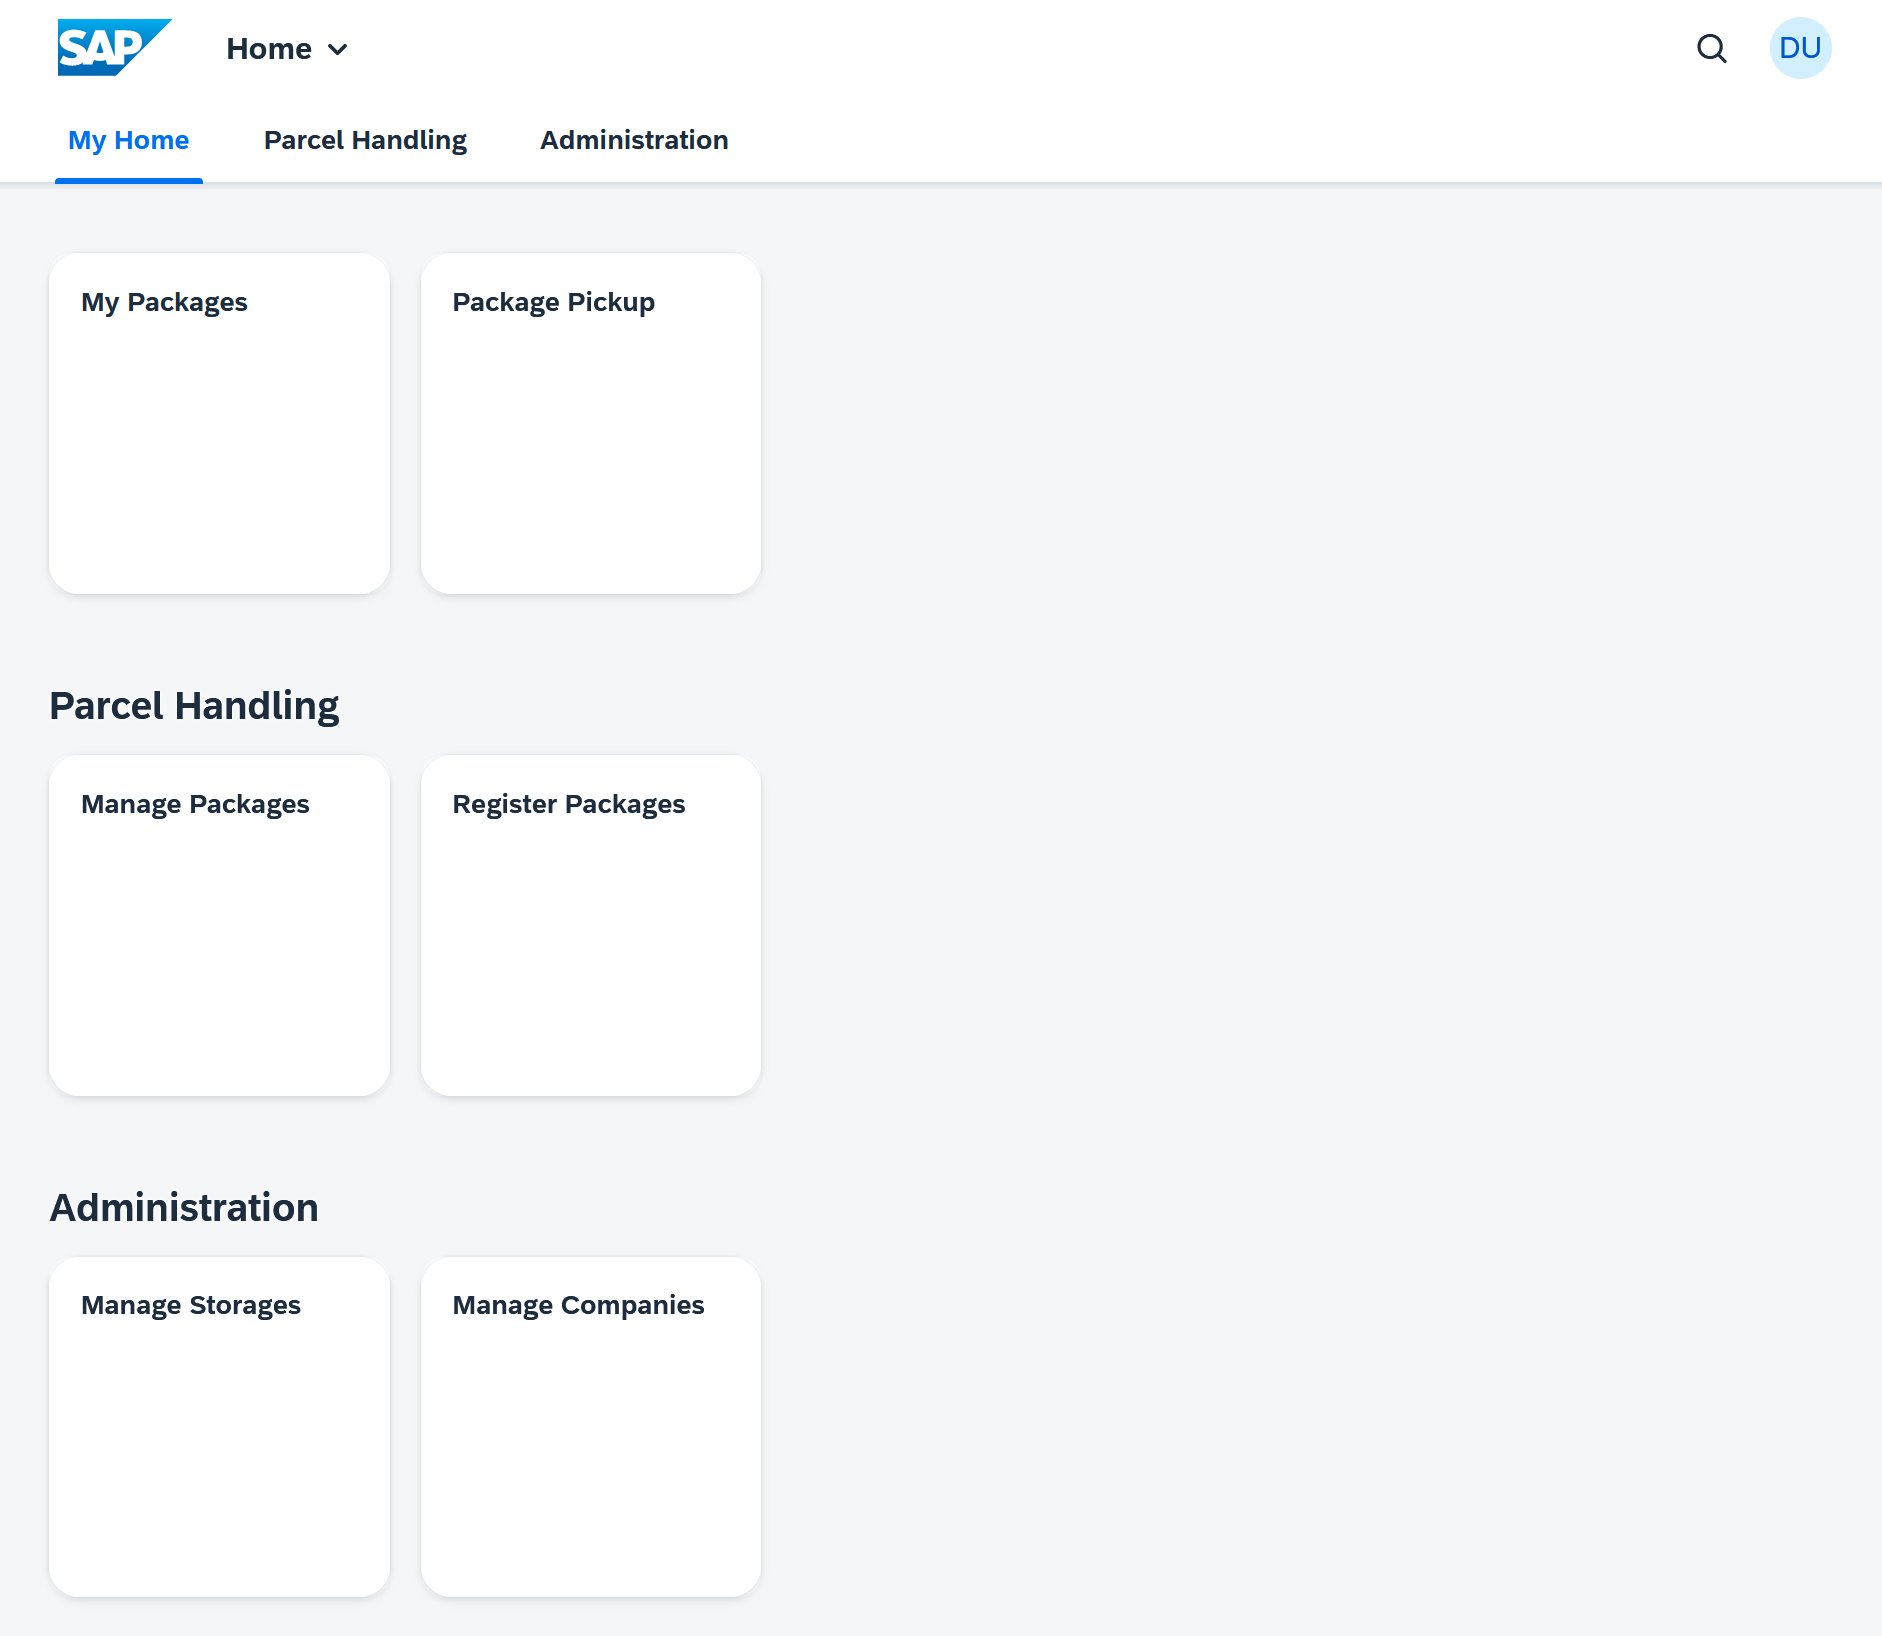
\includegraphics[width=0.95\linewidth]{images/user_doc/lanchpadNewNew.png}
	\caption{Application Launch Screen}
	\label{fig:ApplicationLaunchScreen}
\end{figure}

\section{General Requisite}
\label{sec:GeneralRequisite}
In order to use any of the deployed applications (the deployment is out of scope of this thesis and should be carried on only after), a user has to hold an SAP registered device (computer/tablet/phone) and has to use a supported browser (determined by SAP) with stable internet connection. In order to use \textbf{Pickup packages} application, a user has to hold a smart phone registered by SAP. 

To mock the project in local environment, please first move to the developer documentation (\autoref{sec:D-env}) and checkout the tools and the minimum software version. After the proper installations, the user can clone the repository and install the necessary node modules (\autoref{src:5020}). At this point, the project can be opened and run as specified in \autoref{sec:D-run}.

\lstset{caption={Commands for Local Running of the Solution}, label=src:5020}
\begin{lstlisting}[language={bash}]
> git clone https://github.com/longlegpenguin/parcel-collection-app 
> npm install # install the required node js modules 
\end{lstlisting}

% > git clone https://github.tools.sap/DigitalLabHungary/packagehandling.git # need permission from SAP
The project specifies four different roles: end user, receptionist, facility manager, and administrator. An authenticated user is restricted to accessing project applications dedicated to their assigned role only. The assignment of the roles will be done centrally by a dedicated security component on the BTP (Business Technology Platform) \cite{btp}, where the solution is planned to be deployed (out of scope of this thesis). In the upcoming sections the documentation is sectioned by these roles. Herein, the meanings of each role within the thesis context are listed. Readers can navigate to the relevant sections by clicking on the provided section links.

\begin{description}
	\item[End User (\autoref{sec:UdocEndUser})] Any SAP employee who holds an SAP registered device and would like to use the parcel collection service.
	\item[Receptionist (\autoref{sec:UdocReceptionist})] Registered receptionist working at the reception and is responsible to serve the parcel collection service. Assigned "Receptionist" role on BTP.
	\item[Facility Manager (\autoref{sec:UdocFacilityManager})] Authorised user who is responsible for maintaining the delivery companies and storage slots information. Assigned "FacilityManager" role on BTP.
	\item[Administrator (\autoref{sec:UdocAdministrator})] The master user who can access any of the applications. Assigned "Administrator" role on BTP.
\end{description}

In case the user is accessing the project applications through browser from BTP \cite{btp}, the login process is done automatically. Otherwise, if a user is running the project locally, a browser pop up will be displayed (\autoref{fig:LocalLoginPopUp}) and a mock user (see existing mock credentials in \autoref{sec:D-security}) should be entered.
If any user trying to access an unauthorised application of the project, then the connection will fail (\autoref{fig:IllegalAccesstoUnauthorised Applications}). 

\begin{figure}[H]
	\centering
	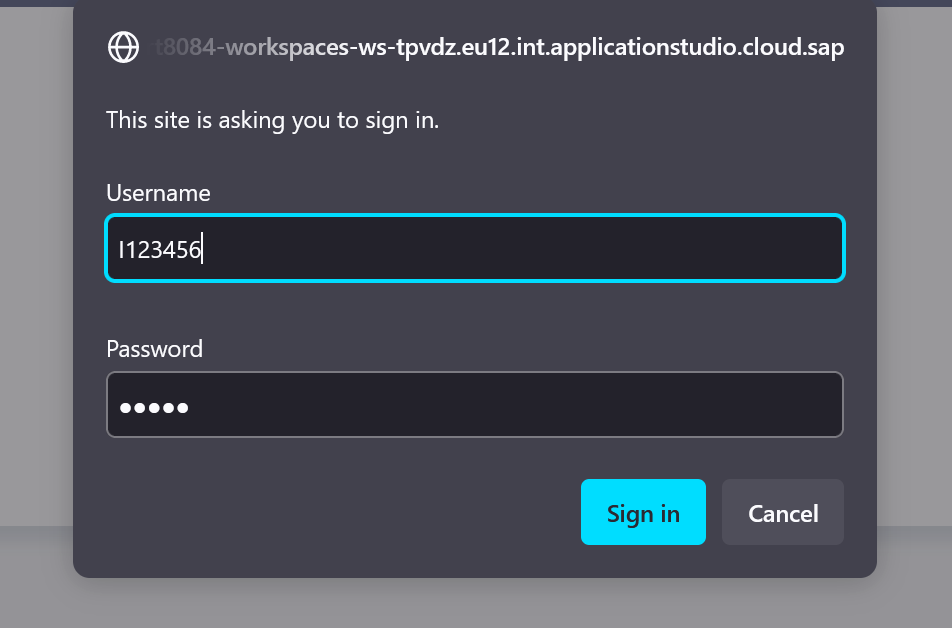
\includegraphics[width=0.6\linewidth]{images/user_doc/overviews/localLogin.png}
	\caption{Local Login Pop Up}
	\label{fig:LocalLoginPopUp}
\end{figure}

\begin{figure}[H]
	\centering
	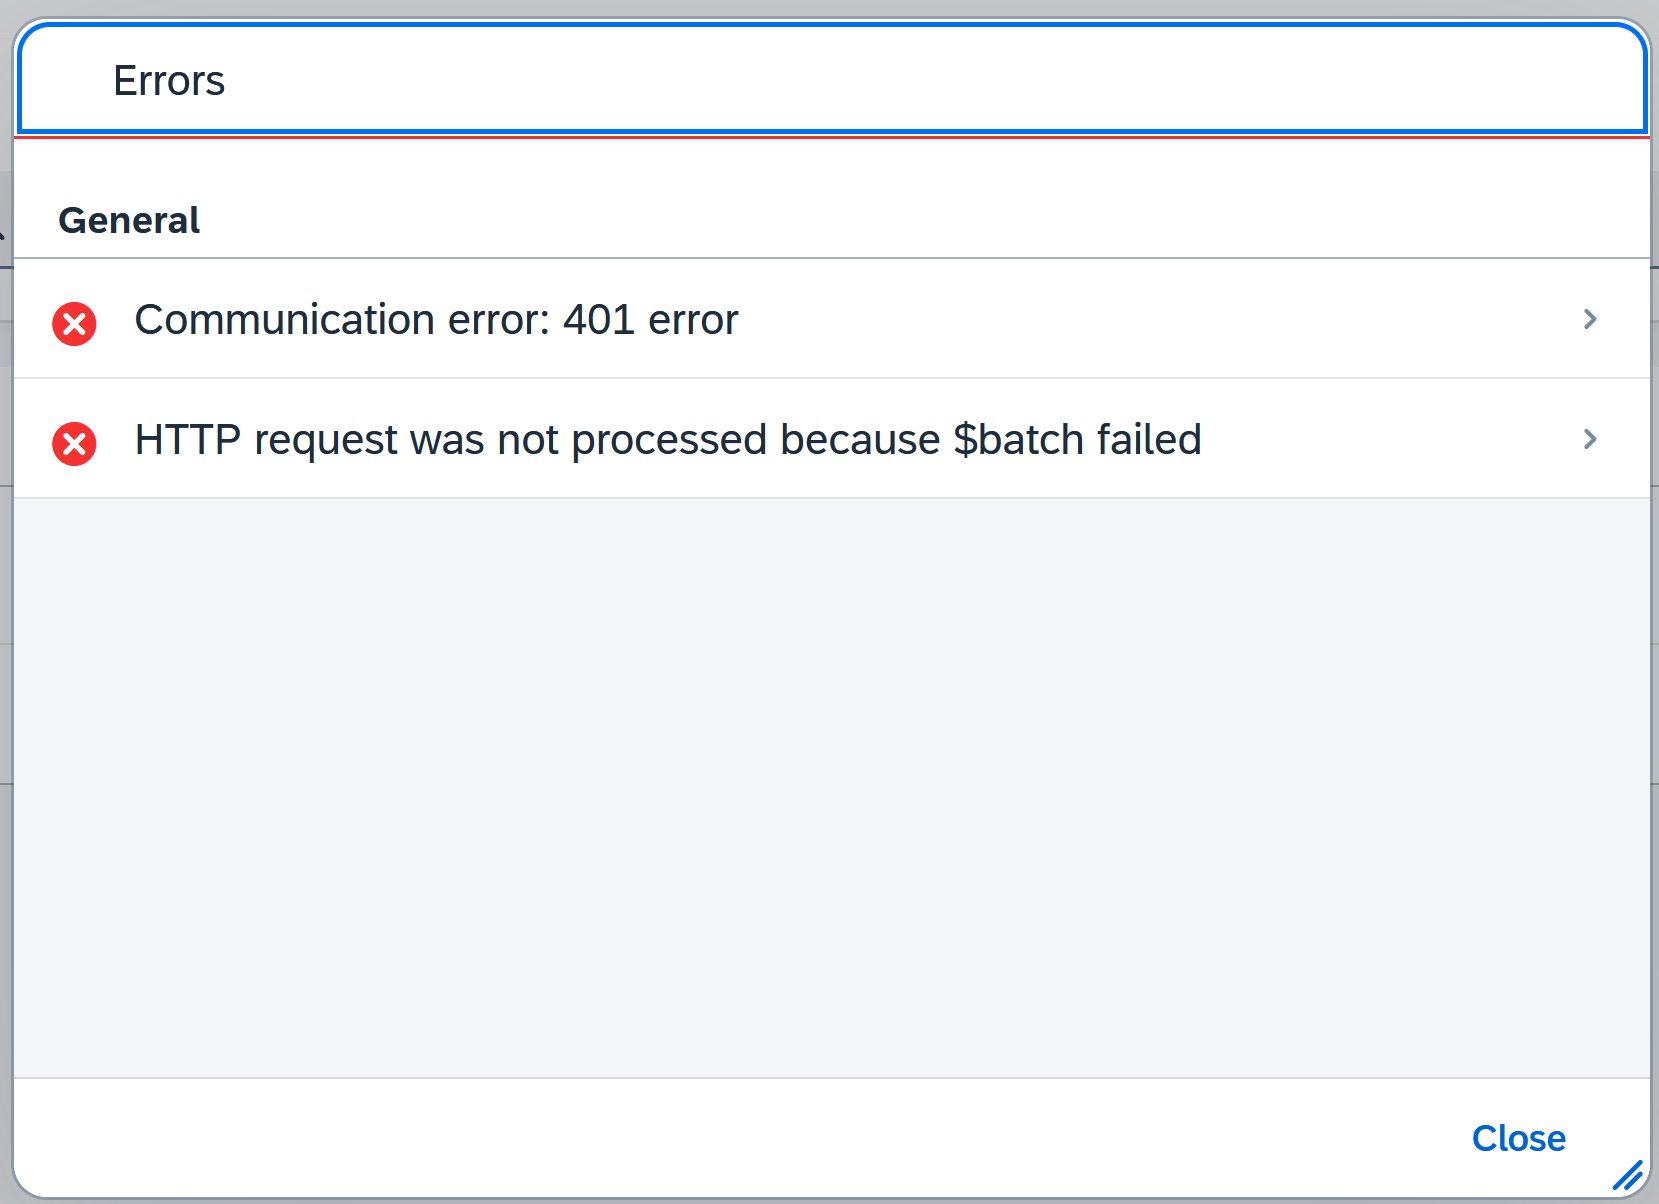
\includegraphics[width=0.6\linewidth]{images/user_doc/overviews/ConnectionError1.png}
	\caption{Illegal Access to Unauthorised Applications - Possible Error}
	\label{fig:IllegalAccesstoUnauthorised Applications}
\end{figure}

\pagebreak

\section{End User}
\label{sec:UdocEndUser}

The \textbf{End User} is granted to access the two applications under the \textbf{My Home} section, namely \textbf{My Packages} (\autoref{subsec:ph}) and \textbf{Package Pickup} (\autoref{subsec:pp}). An \textbf{End User} can quick jump to the section by left clicking the "My Home" tab. Applications can be entered by left clicking the tiles (\autoref{fig:EndUserApplications}).

\begin{figure}[H]
	\centering
	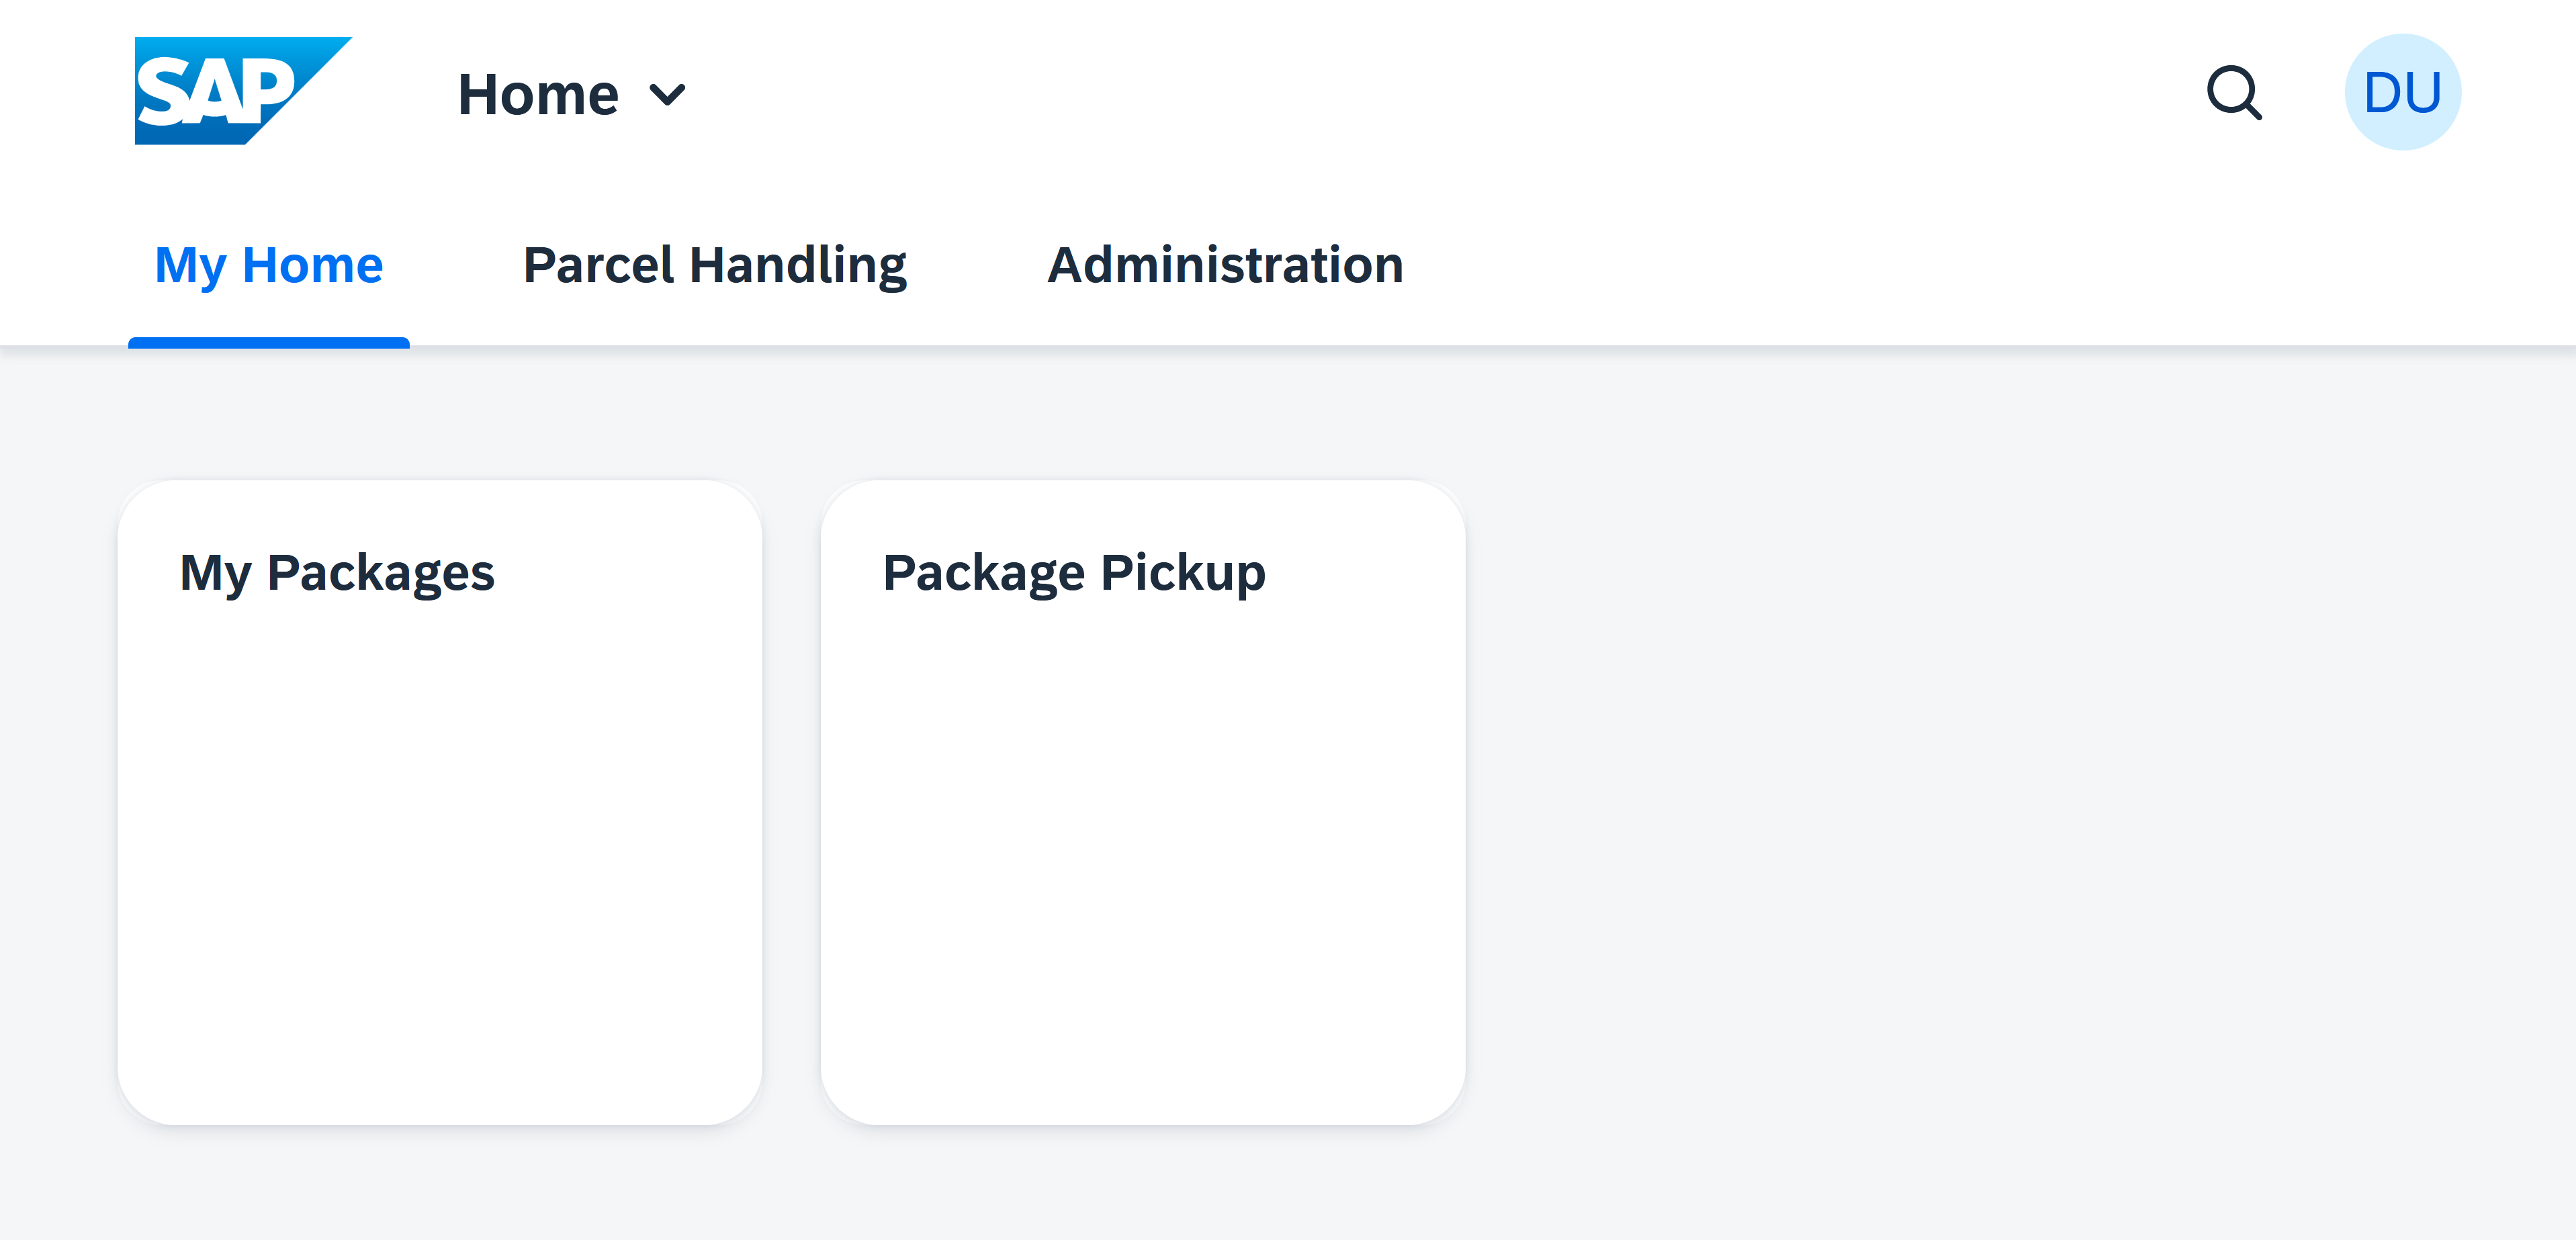
\includegraphics[width=1\linewidth]{images/user_doc/overviews/MyHomeTab.png}
	\caption{End User Applications}
	\label{fig:EndUserApplications}
\end{figure}


% ----------------------- MY PACKAGES ----------------------------
% 
%  ---------------------------------------------------------------

\subsection{My Packages}
\label{subsec:ph}

The \textbf{My Packages} application is here for any \textbf{End User} (see \autoref{sec:UdocEndUser} for all related applications) who would want to check his/her own packages. The reader can navigate to \autoref{subsec:dev-ui-ph} for more implementation details.
The summarized main actions that can be taken within the application are listed here:

\begin{compactenum}
	\item Browse the owned package history.
        \begin{compactenum}
        	\item Filter possibility.
            \item List report for packages.
        \end{compactenum}
\end{compactenum}

\subsubsection{Home Screen - Overview}
An \textbf{End User}, after clicking at the application tile, is redirected to the "Home Screen" (\autoref{fig:HistoryHome}), which is the main screen of this application. The upper part displays the search bar and the possible filters. While a list of packages is displayed in the lower part. The information provided for each packages are: \textbf{Type} (the type of the package, existing types are newspaper, letter and normal), \textbf{Status} (the status of the package, existing status are new, confirmed and picked up), \textbf{Delivery Company} (the delivery company of the package), \textbf{Delivery Time} (the confirmation time of the package, if applicable), \textbf{Pickup Time} (the pickup time of the package, if applicable).

\begin{figure}[H]
	\centering
	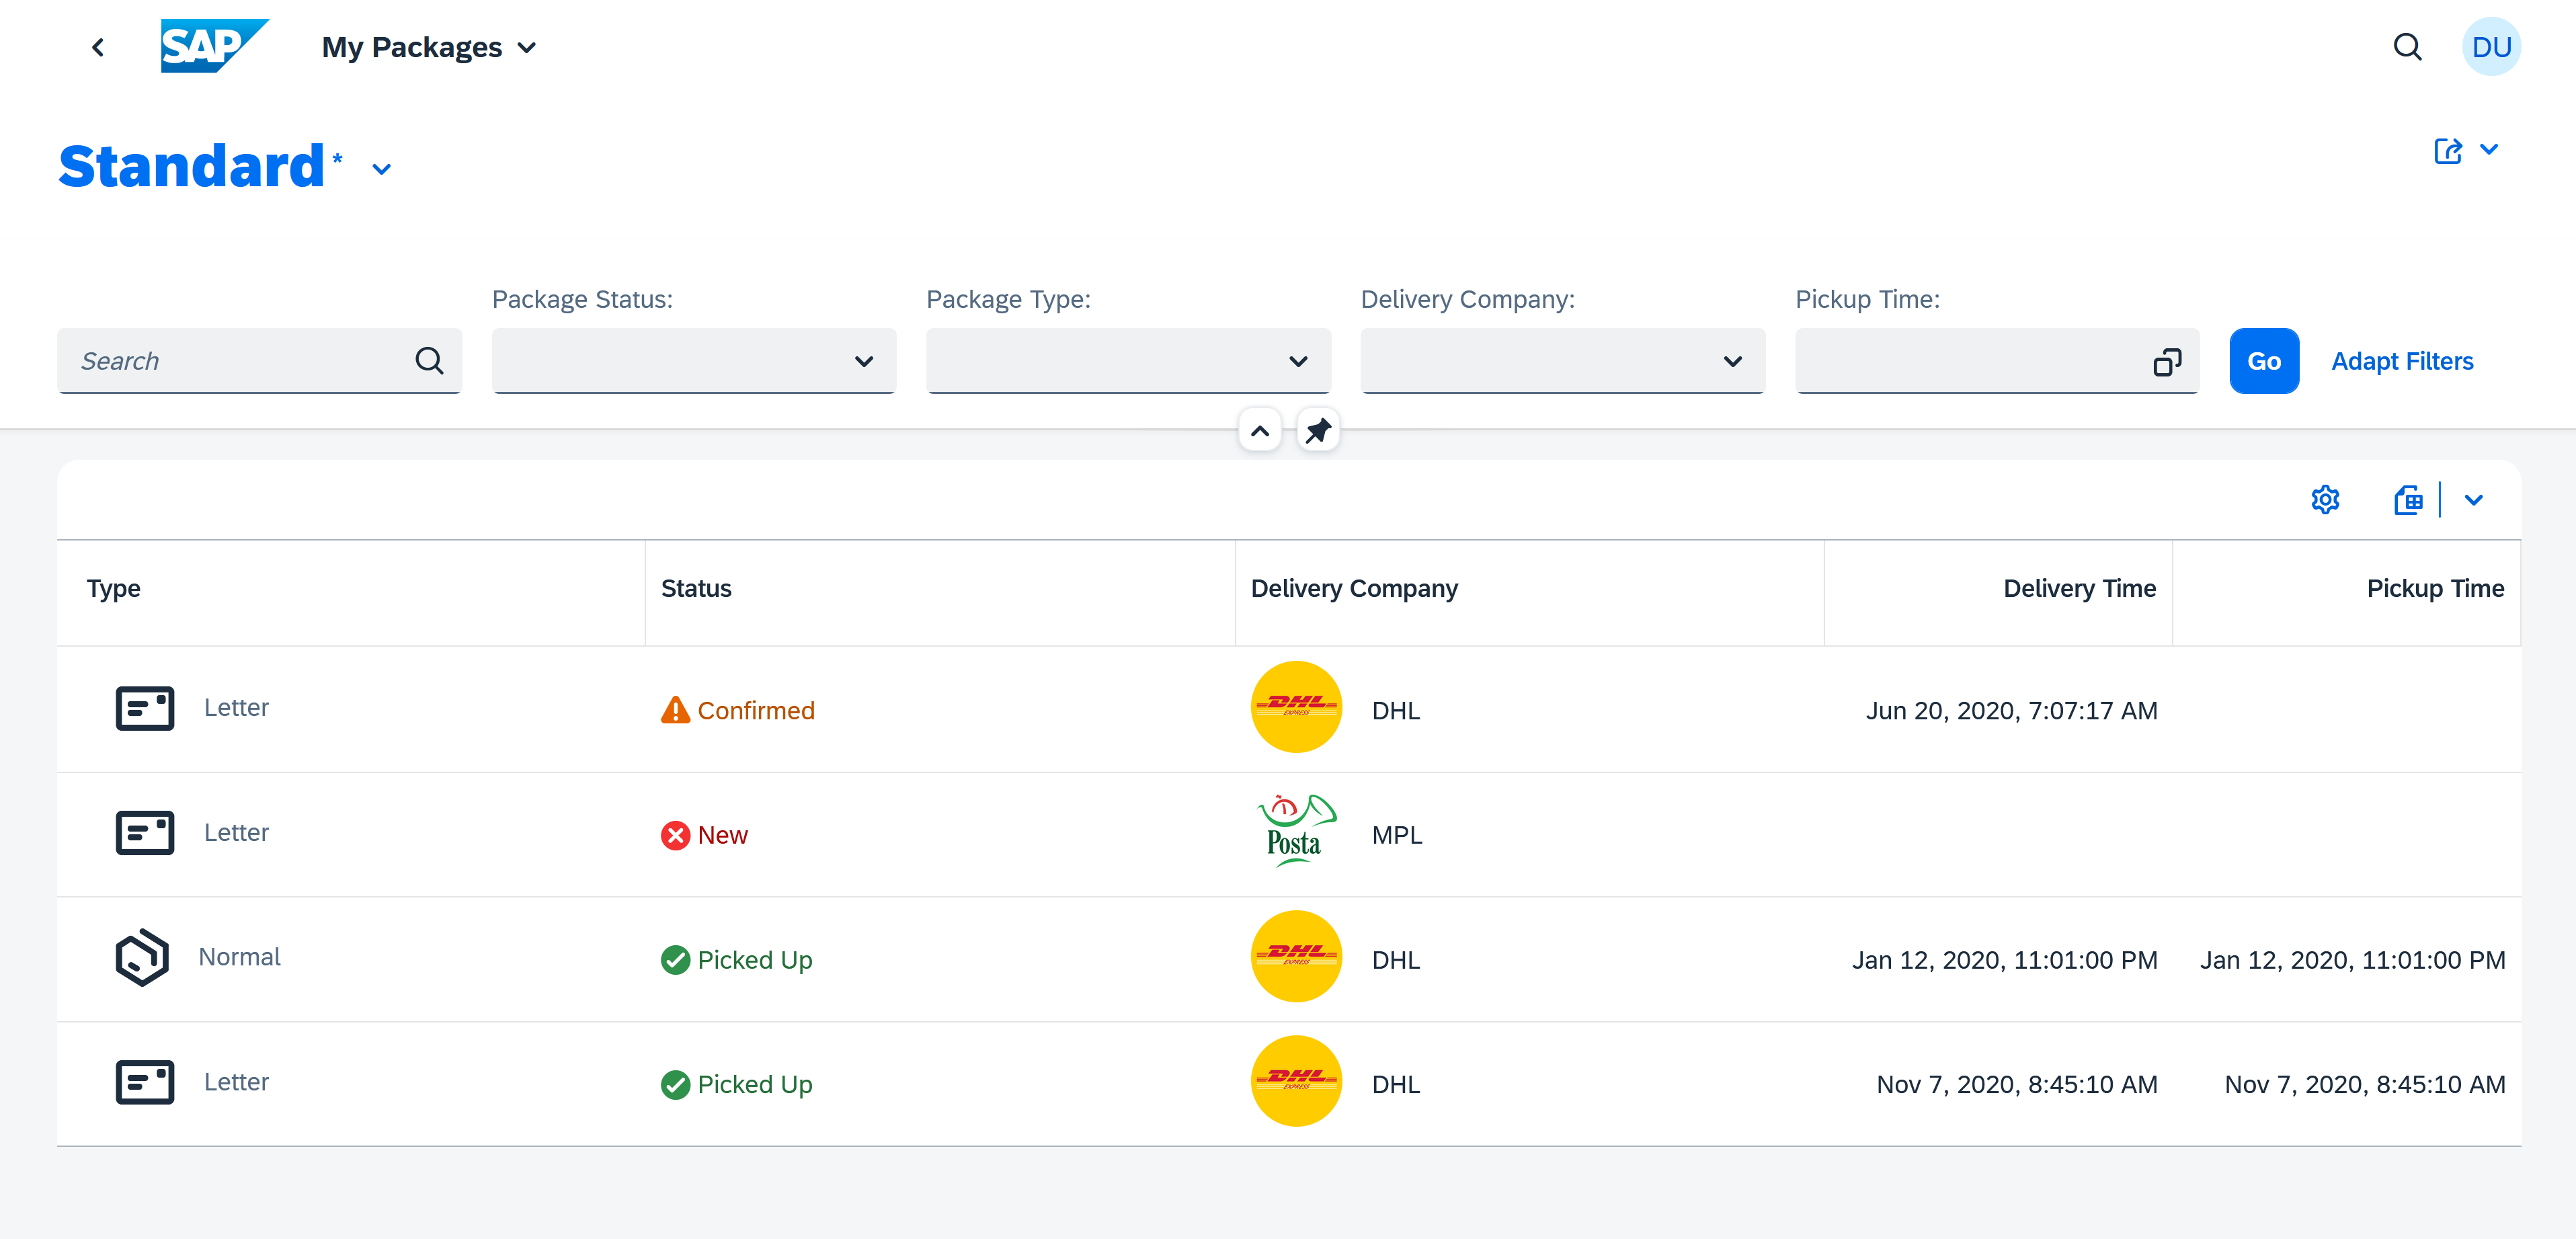
\includegraphics[width=1\linewidth]{images/user_doc/myPack/overview.png}
	\caption{History Home Screen - Overview}
	\label{fig:HistoryHome}
\end{figure}

\subsubsection{Home Screen - Filter Usage}
The user can search for entries by typing in free text of any possible content of the columns in the "Search Bar" (\autoref{fig:mpSearchBar}). The free text supports in-completed keywords and is case insensitive. 
The default filters (\textbf{Status} (drop down), \textbf{Type} (drop down), \textbf{Delivery Company} (drop down) and \textbf{Pickup Time} (time entry) can be used to narrow down the table results (\autoref{fig:MPDF}). 

For any drop down filters, the user can click at the small drop down arrow and select zero to many options. To set the time filter, the user should click at the "double box" (filter help) on the right of the filter box. This will pop up a dialog, at where the user can select the desired filtering option and enter the time with the clock utility (\autoref{fig:PHAjustTimeFilters}). 

More filters (\textbf{Delivery Time} (time entry)) can be accessed by clicking at "Adapt Filters" (\autoref{fig:mpMOreFilterAdaption}). While adjusting the filtering values, the list view is temporarily locked. By clicking the "Go" Button, the adjusted filters are running and results are displayed (\autoref{fig:PHAjustFilters-2}).

\begin{figure}[htb!]
	\centering
	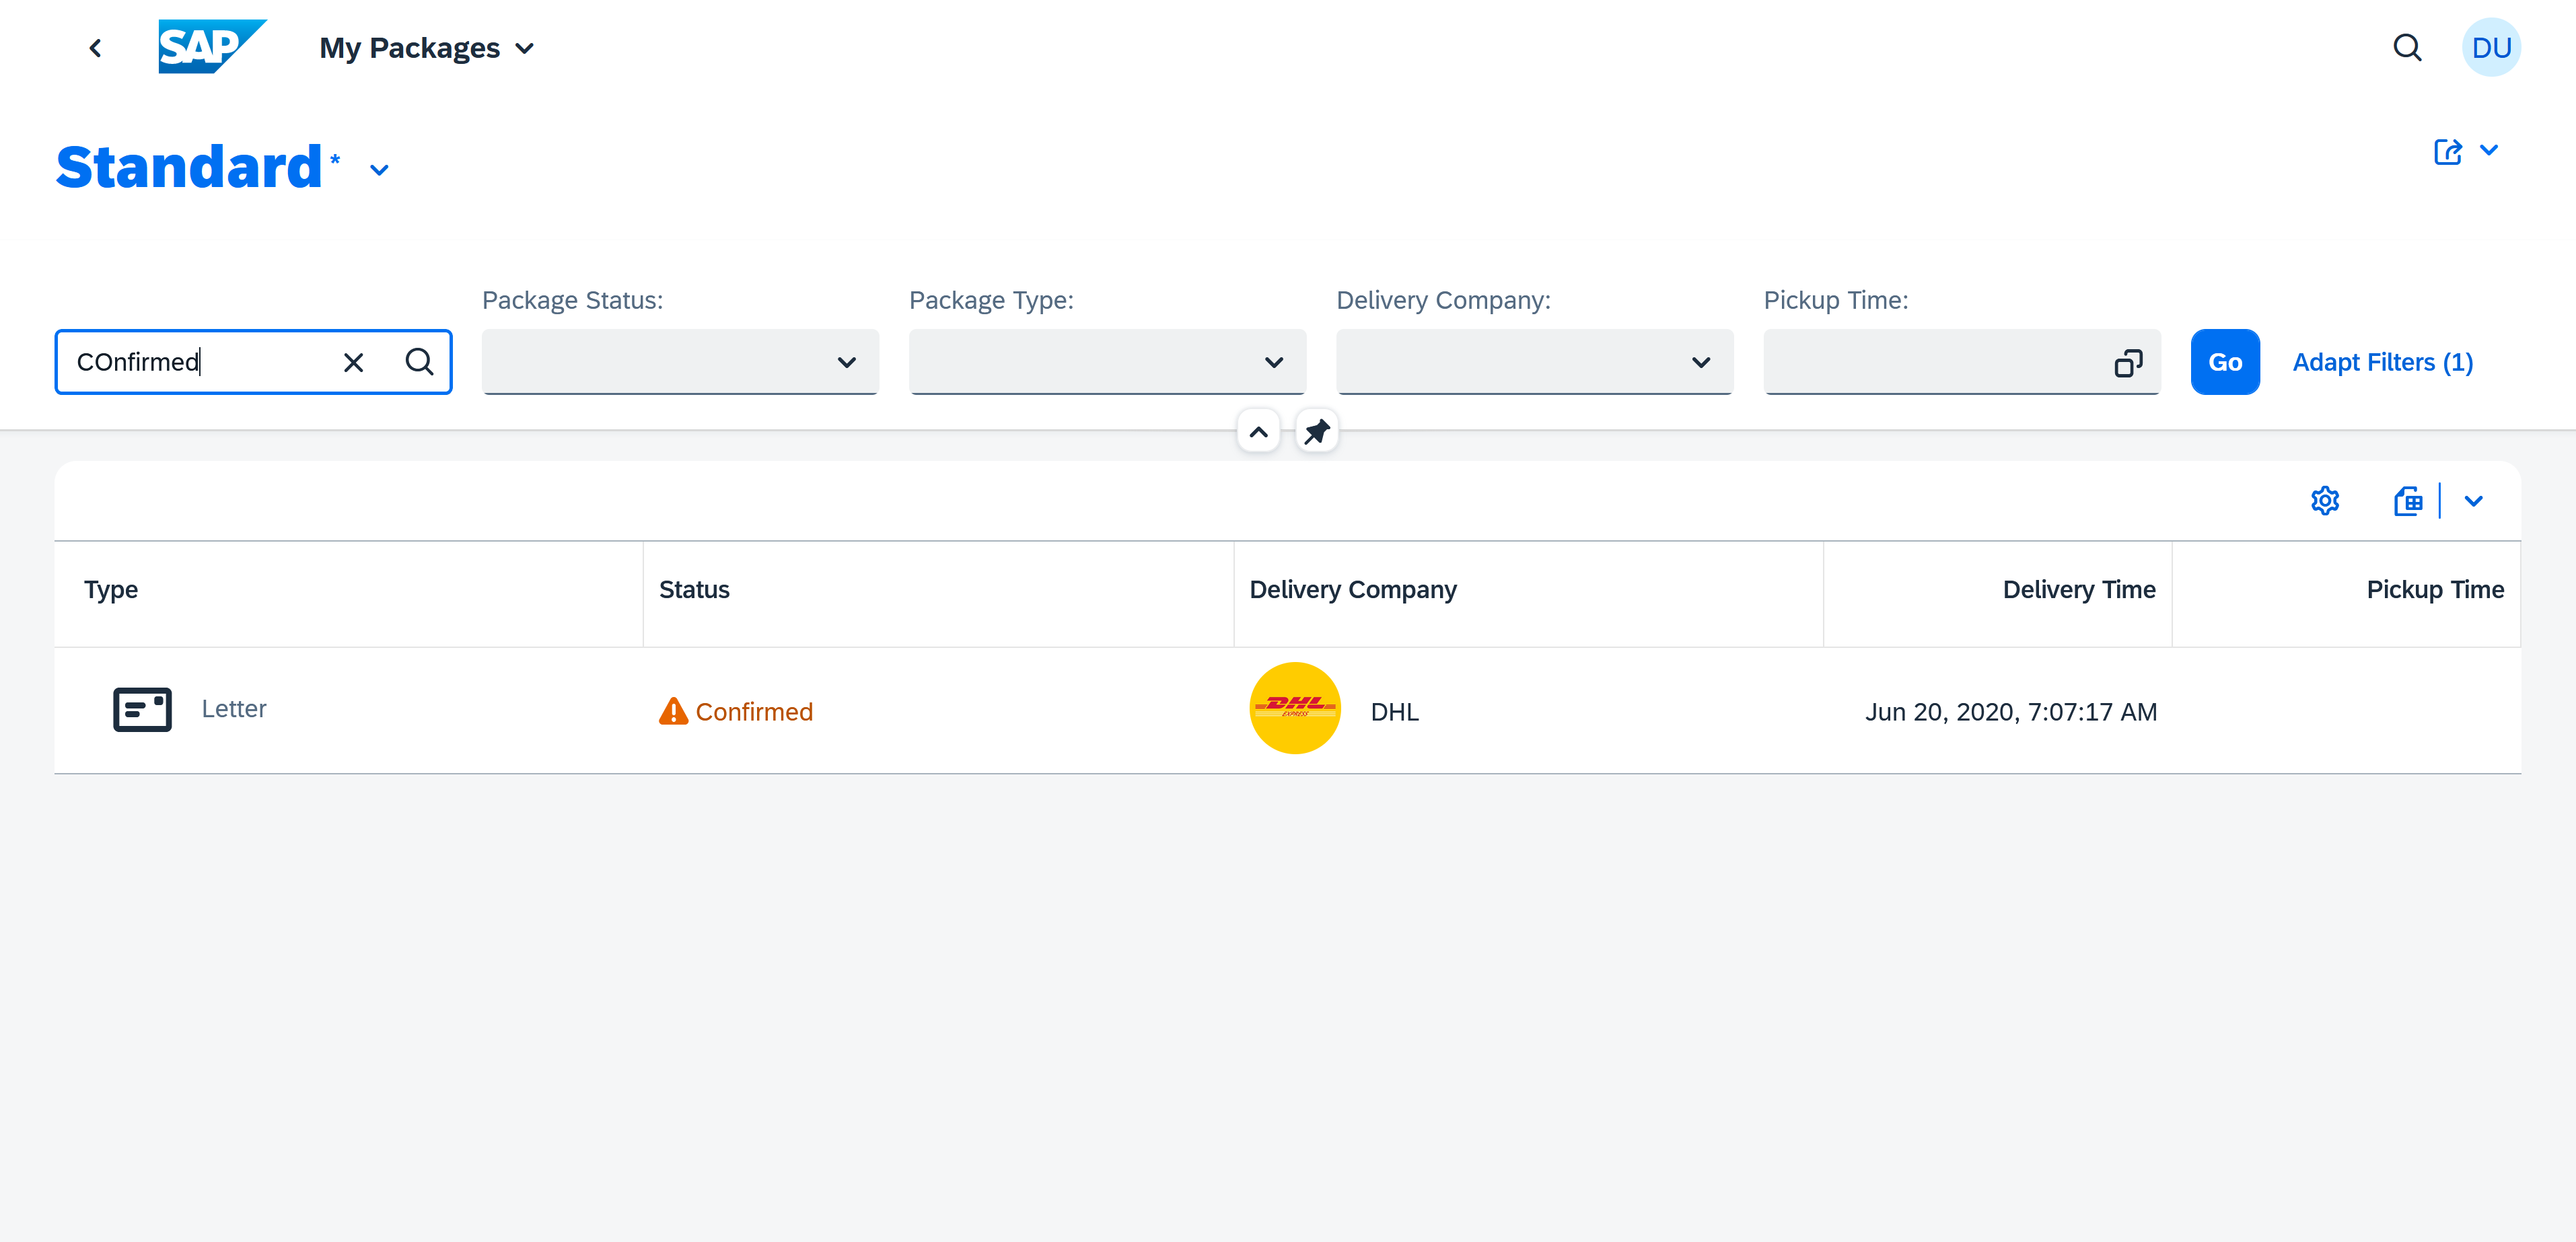
\includegraphics[width=0.9\linewidth]{images/user_doc/myPack/searchbar.png}
	\caption{My Package Home Screen - Search Bar}
	\label{fig:mpSearchBar}
\end{figure}


\begin{figure}[htb!]
	\centering
	\subcaptionbox{Status Filter}{
		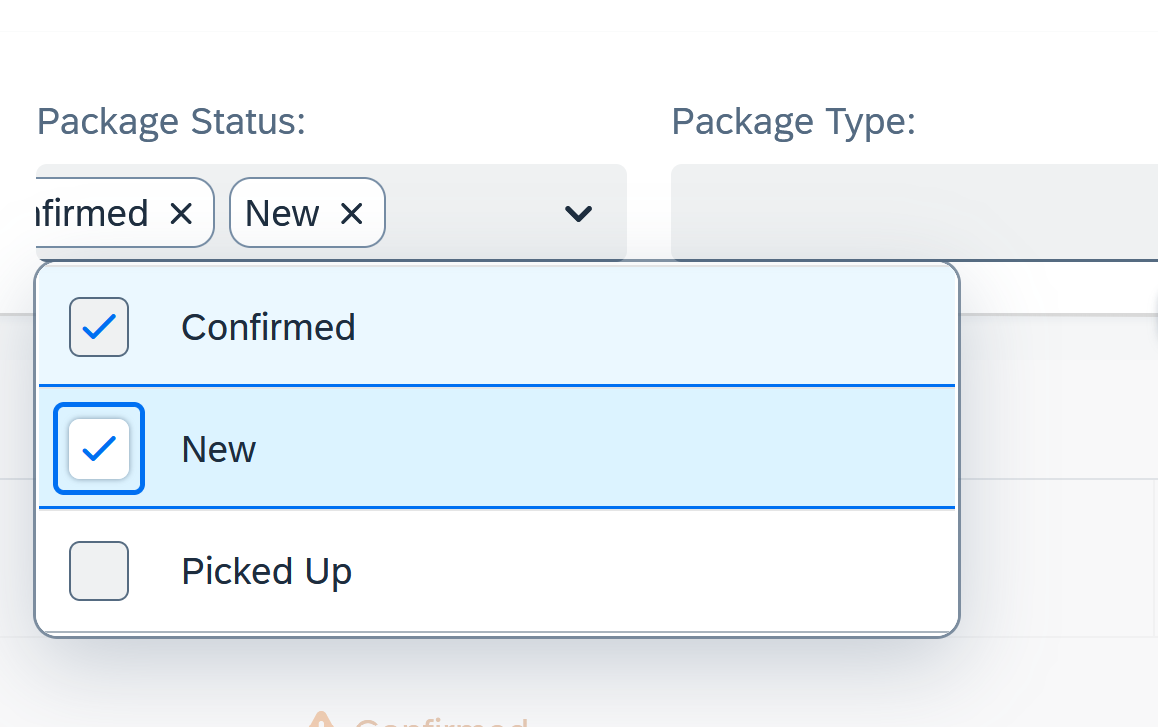
\includegraphics[width=0.45\linewidth]{images/user_doc/myPack/statusFIlter.png}}
	\hspace{5pt}
	\subcaptionbox{Type Filter}{
		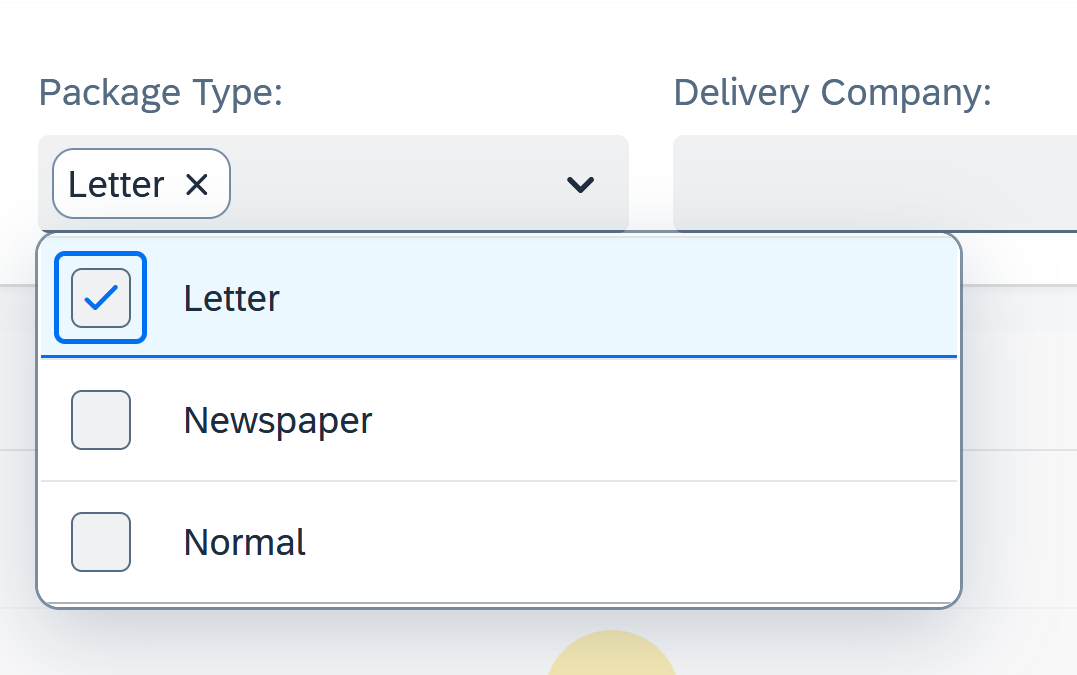
\includegraphics[width=0.45\linewidth]{images/user_doc/myPack/typeFIlter.png}}

    \subcaptionbox{Company Filter}{
		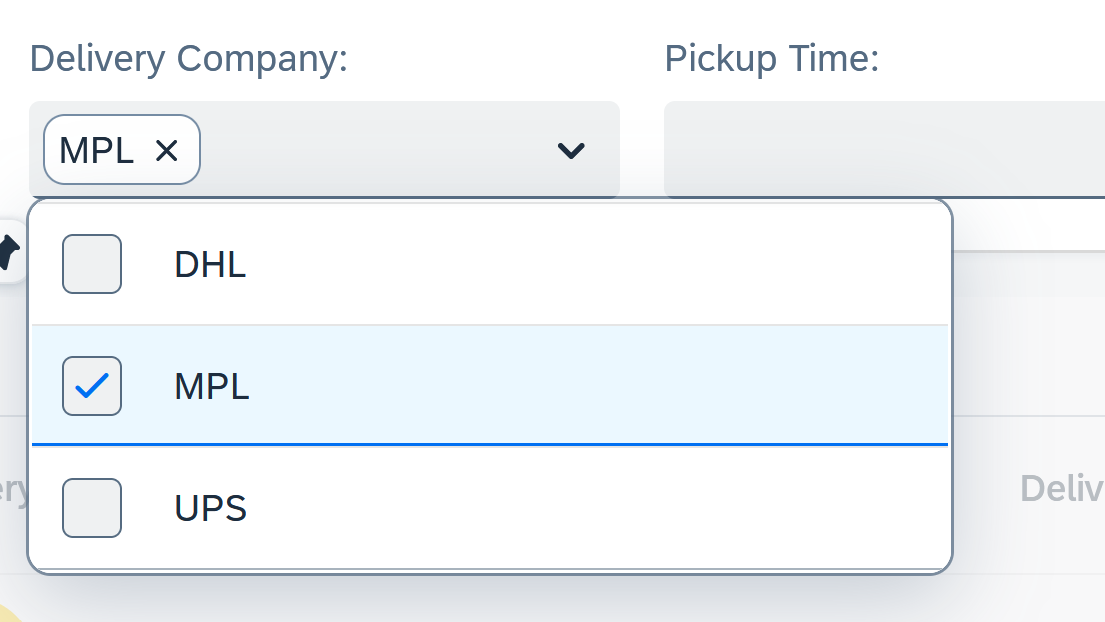
\includegraphics[width=0.45\linewidth]{images/user_doc/myPack/companyFilter.png}}
	\hspace{5pt}
	\subcaptionbox{Time Filter}{
		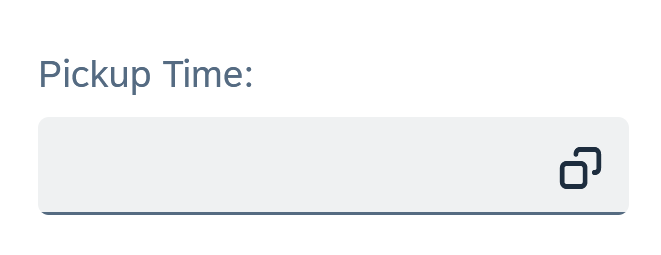
\includegraphics[width=0.45\linewidth]{images/user_doc/myPack/timeFilter.png}}
	\caption{My Package Home Screen - Default Filters}
	\label{fig:MPDF}
\end{figure}

\begin{figure}[H]
		\centering
	\subcaptionbox{Time Filter Options Selections}{
		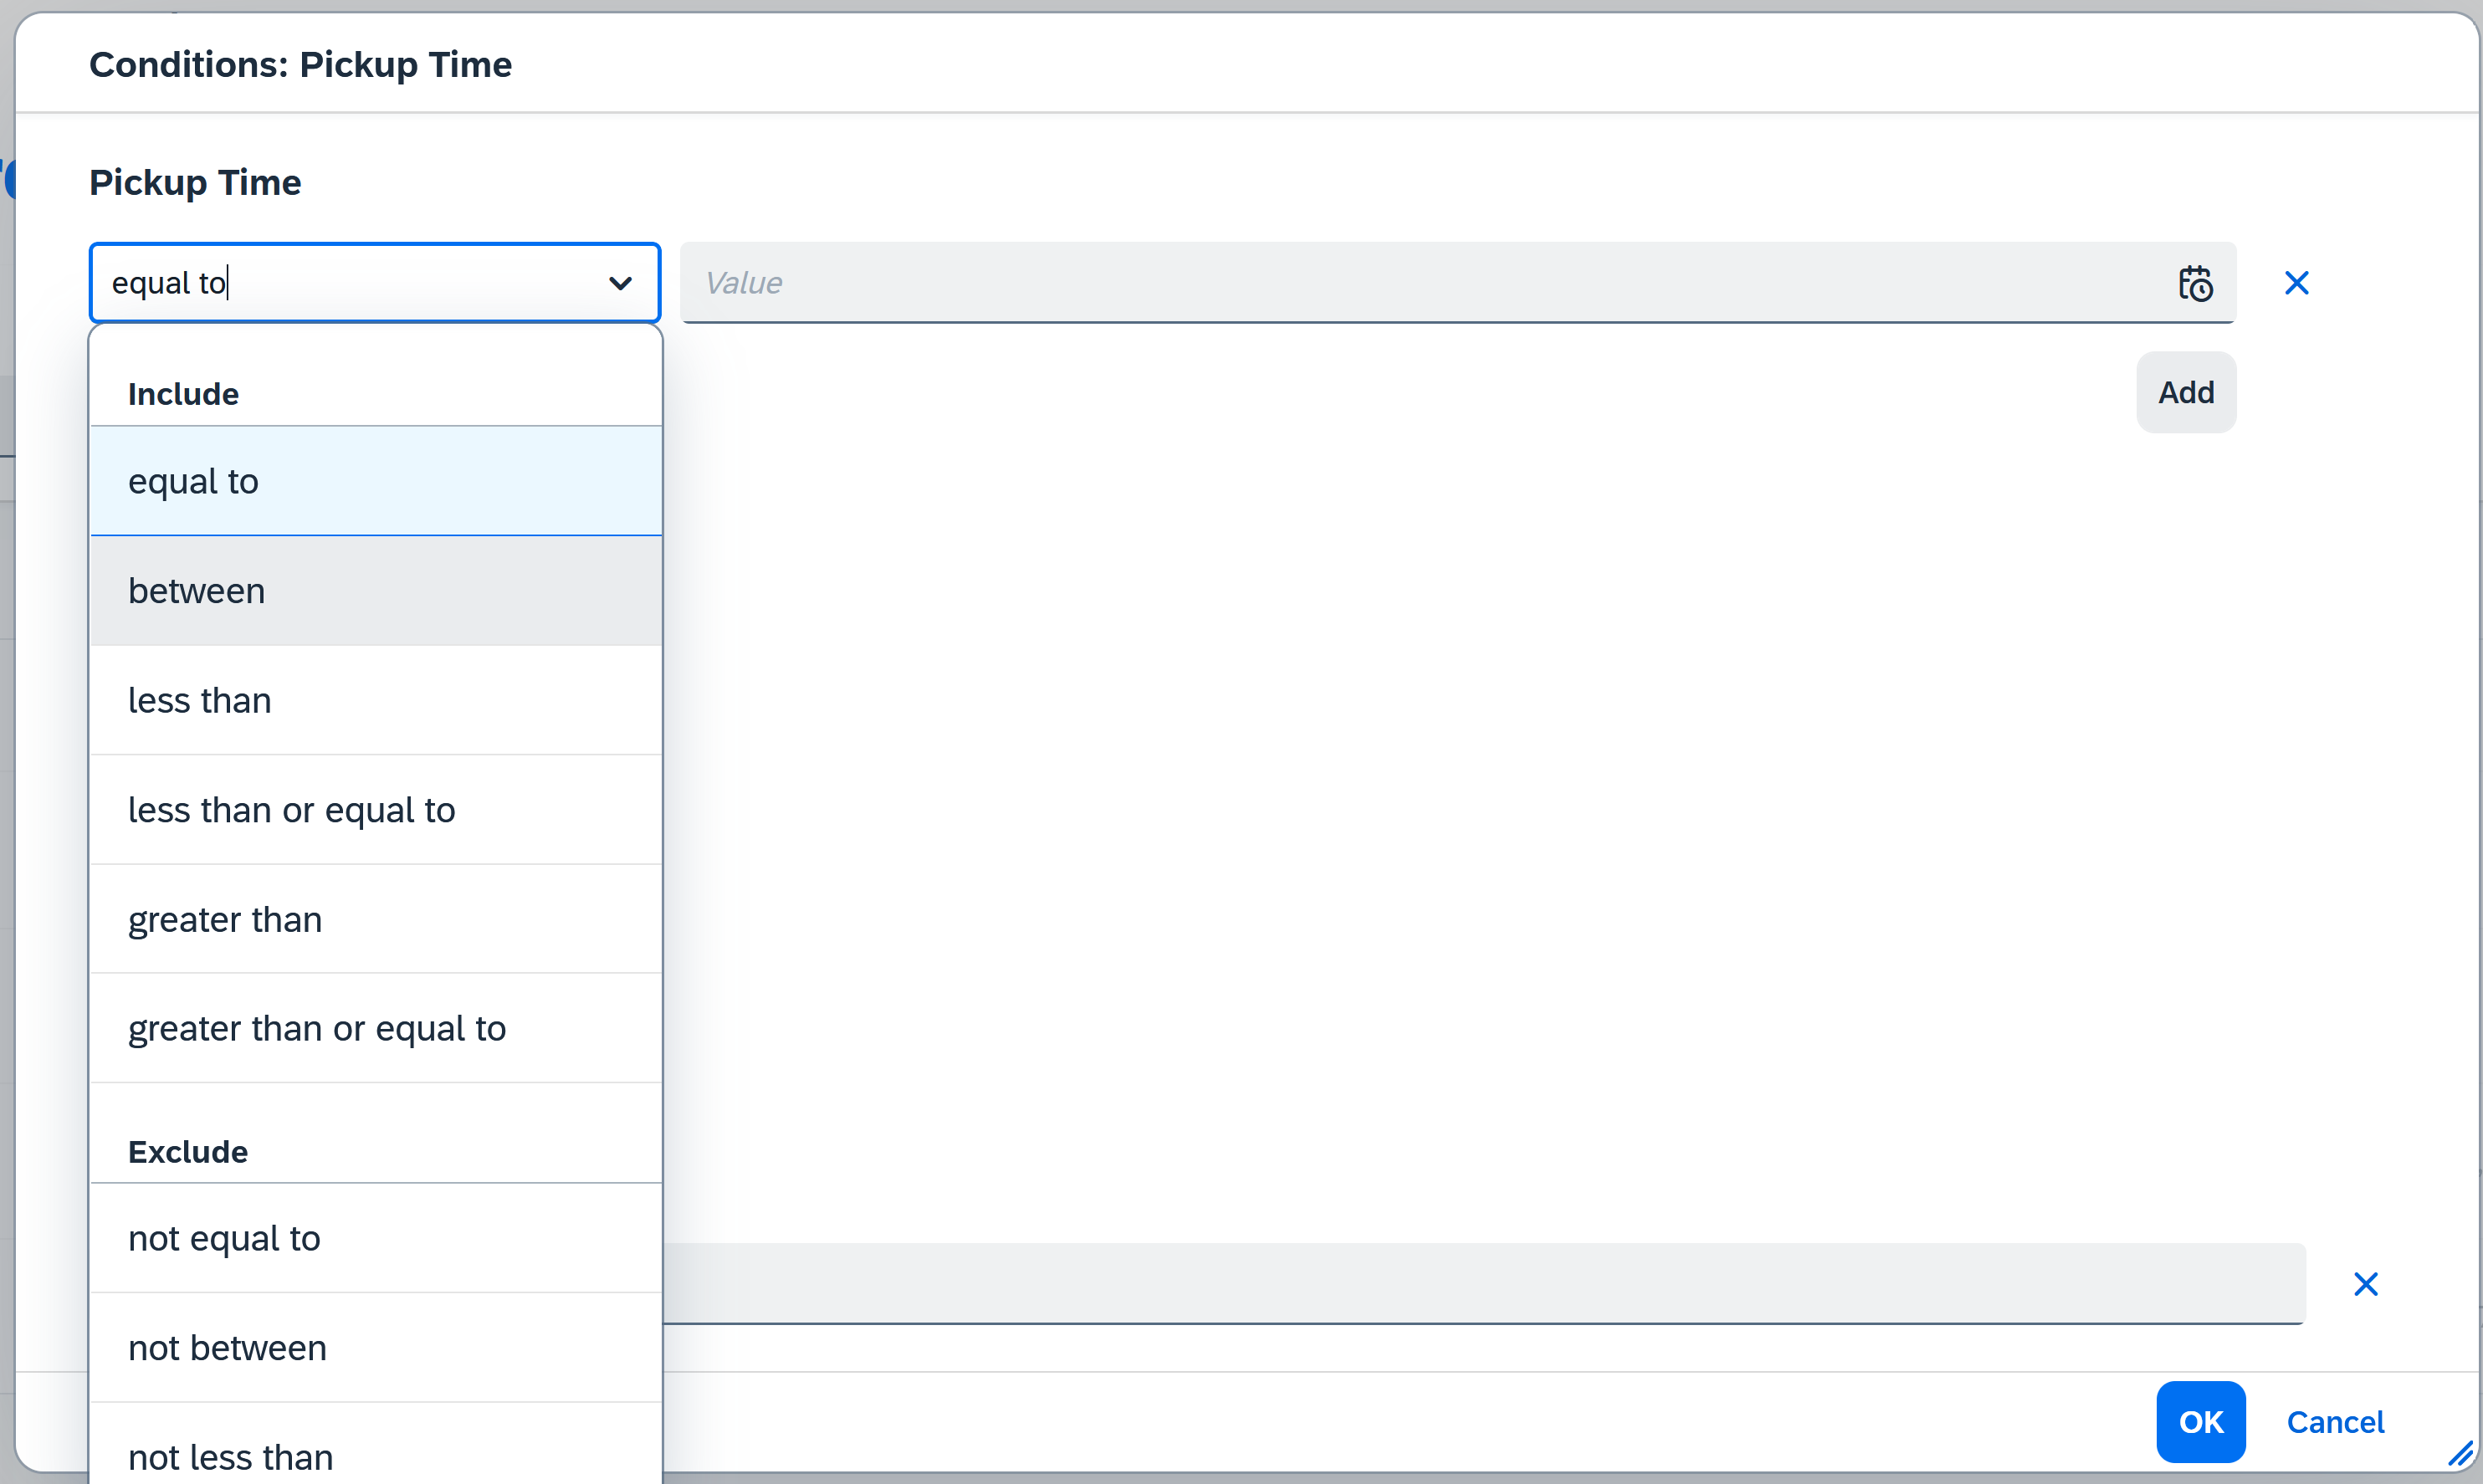
\includegraphics[width=0.45\linewidth]{images/user_doc/myPack/timeFilter_Usage1.png}}
	\hspace{5pt}
	\subcaptionbox{Time Entry}{
		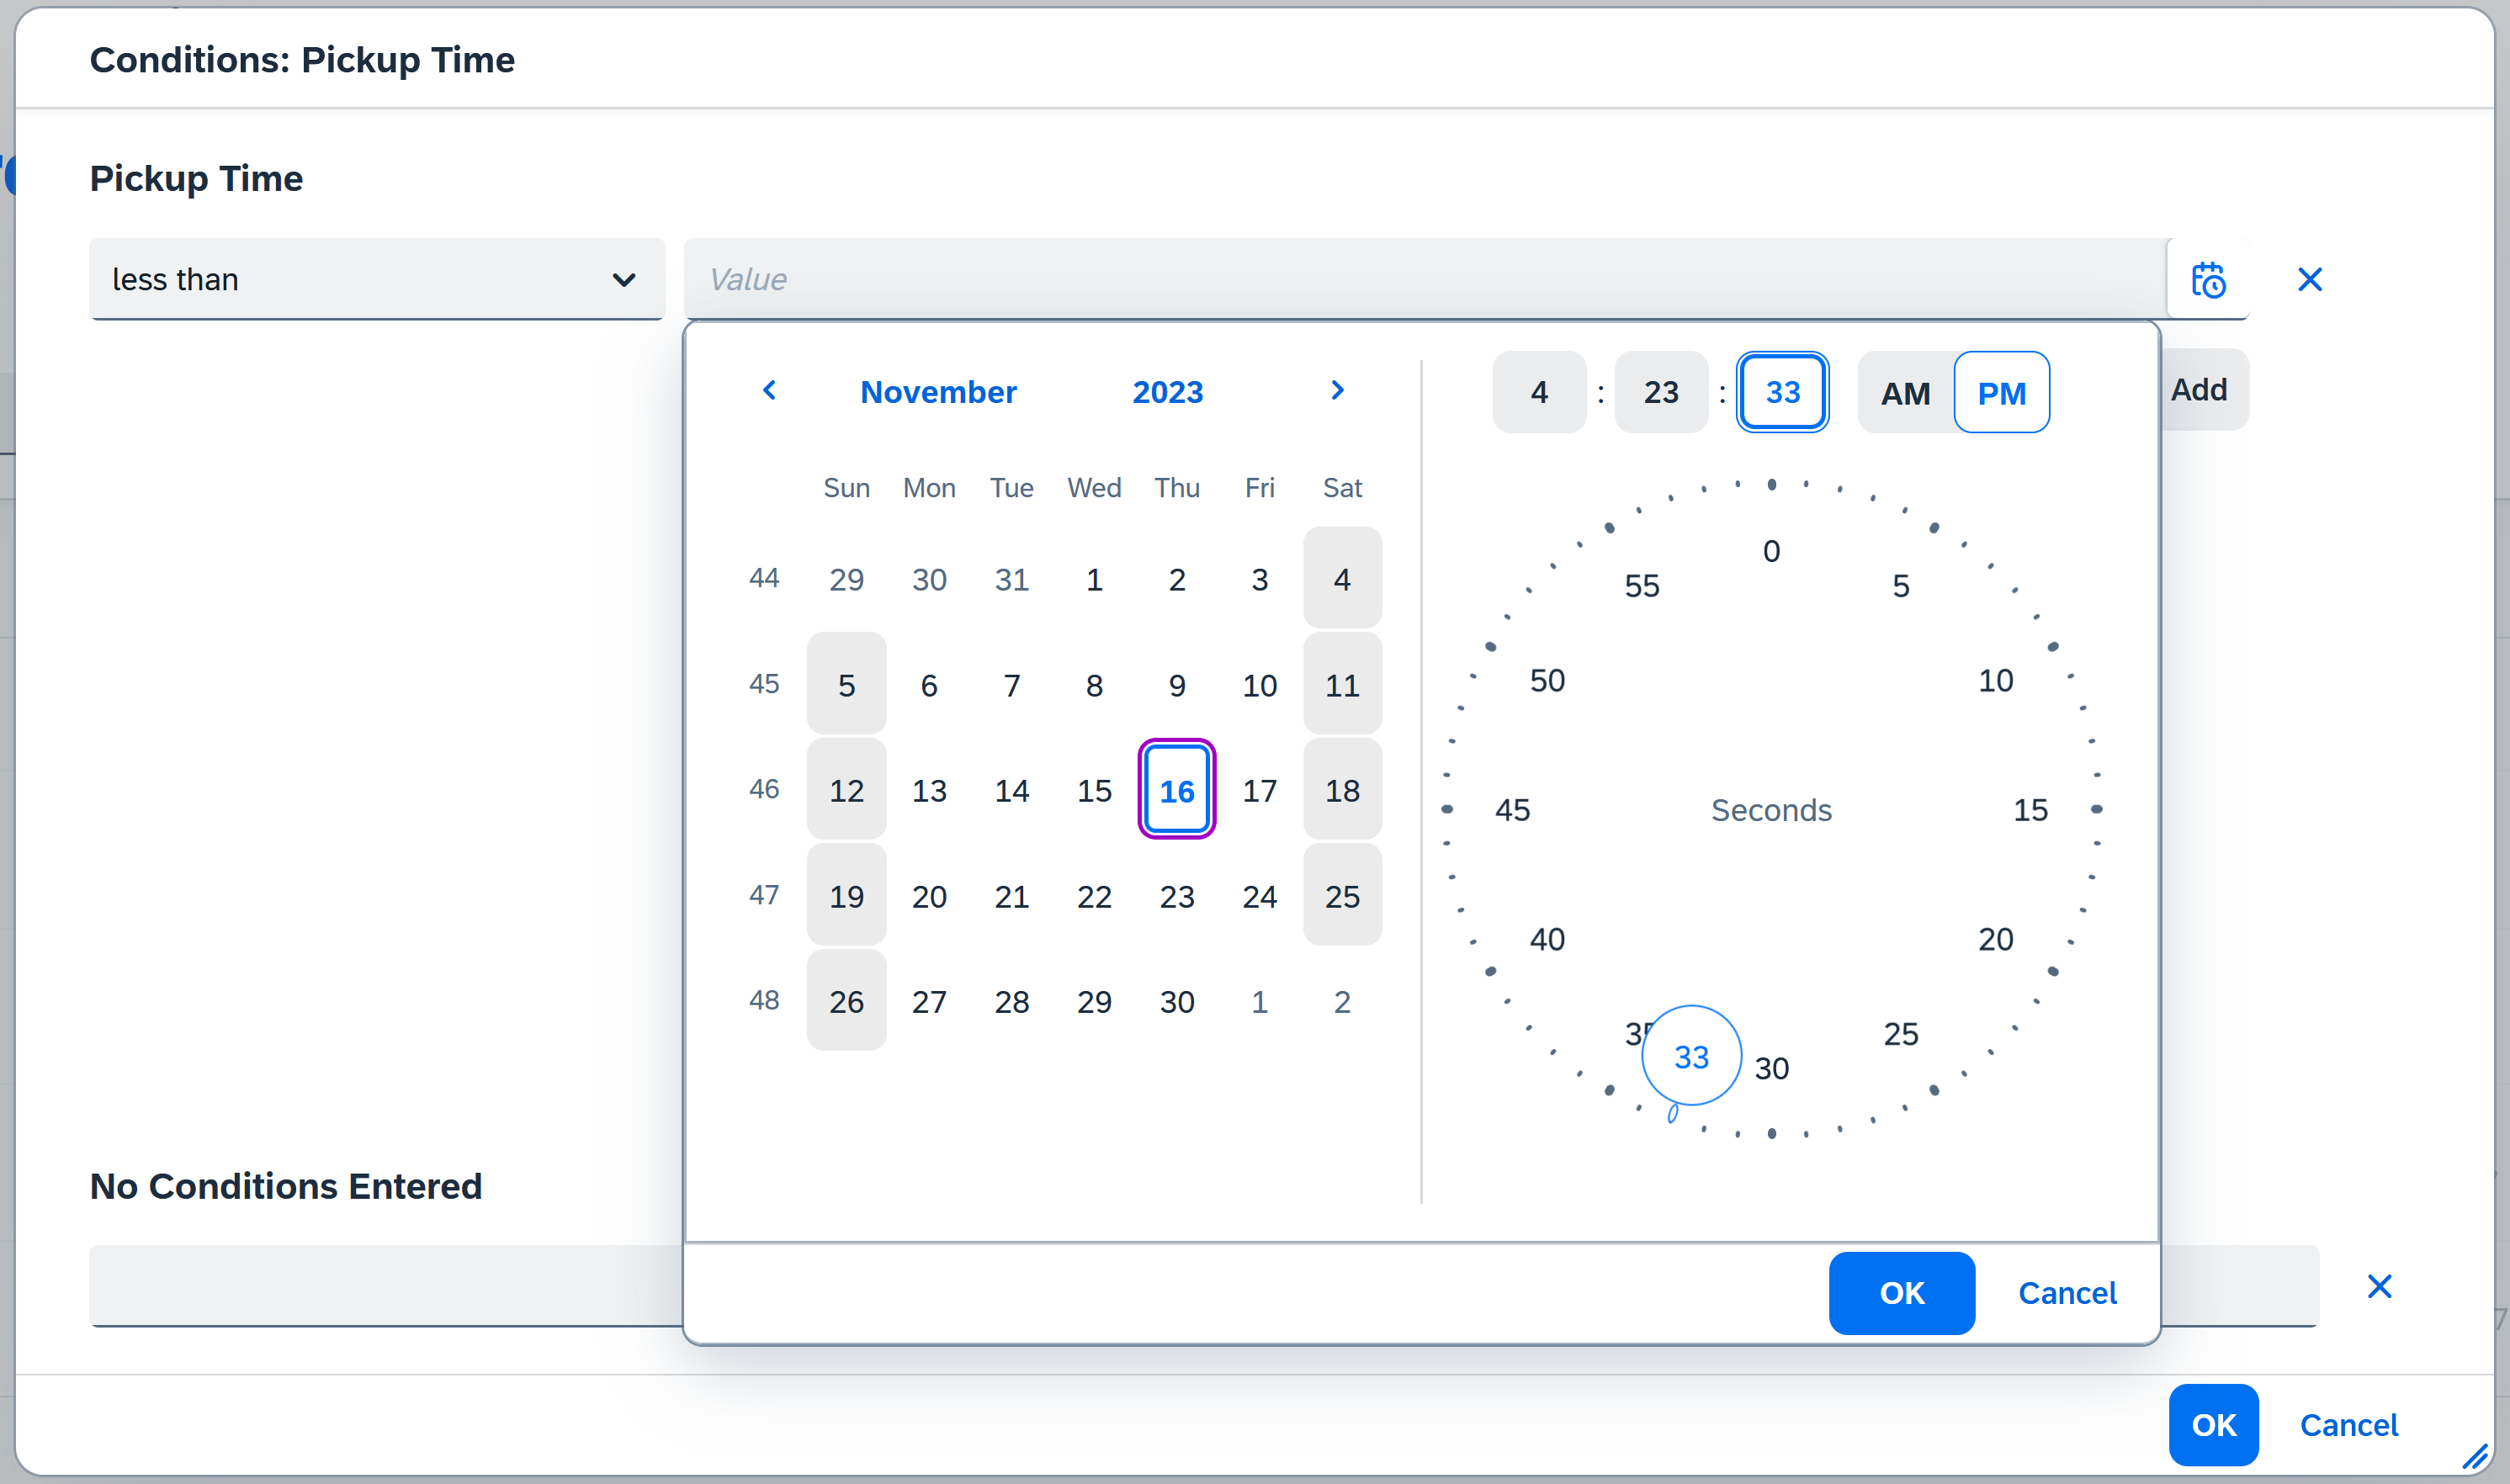
\includegraphics[width=0.45\linewidth]{images/user_doc/myPack/timeFilter-Usage2.png}}
    \caption{Time Filter Dialog - Adjust Filters}
    \label{fig:PHAjustTimeFilters}
\end{figure}


\begin{figure}[htb!]
		\centering
	\subcaptionbox{While Adjusting the Filter}{
		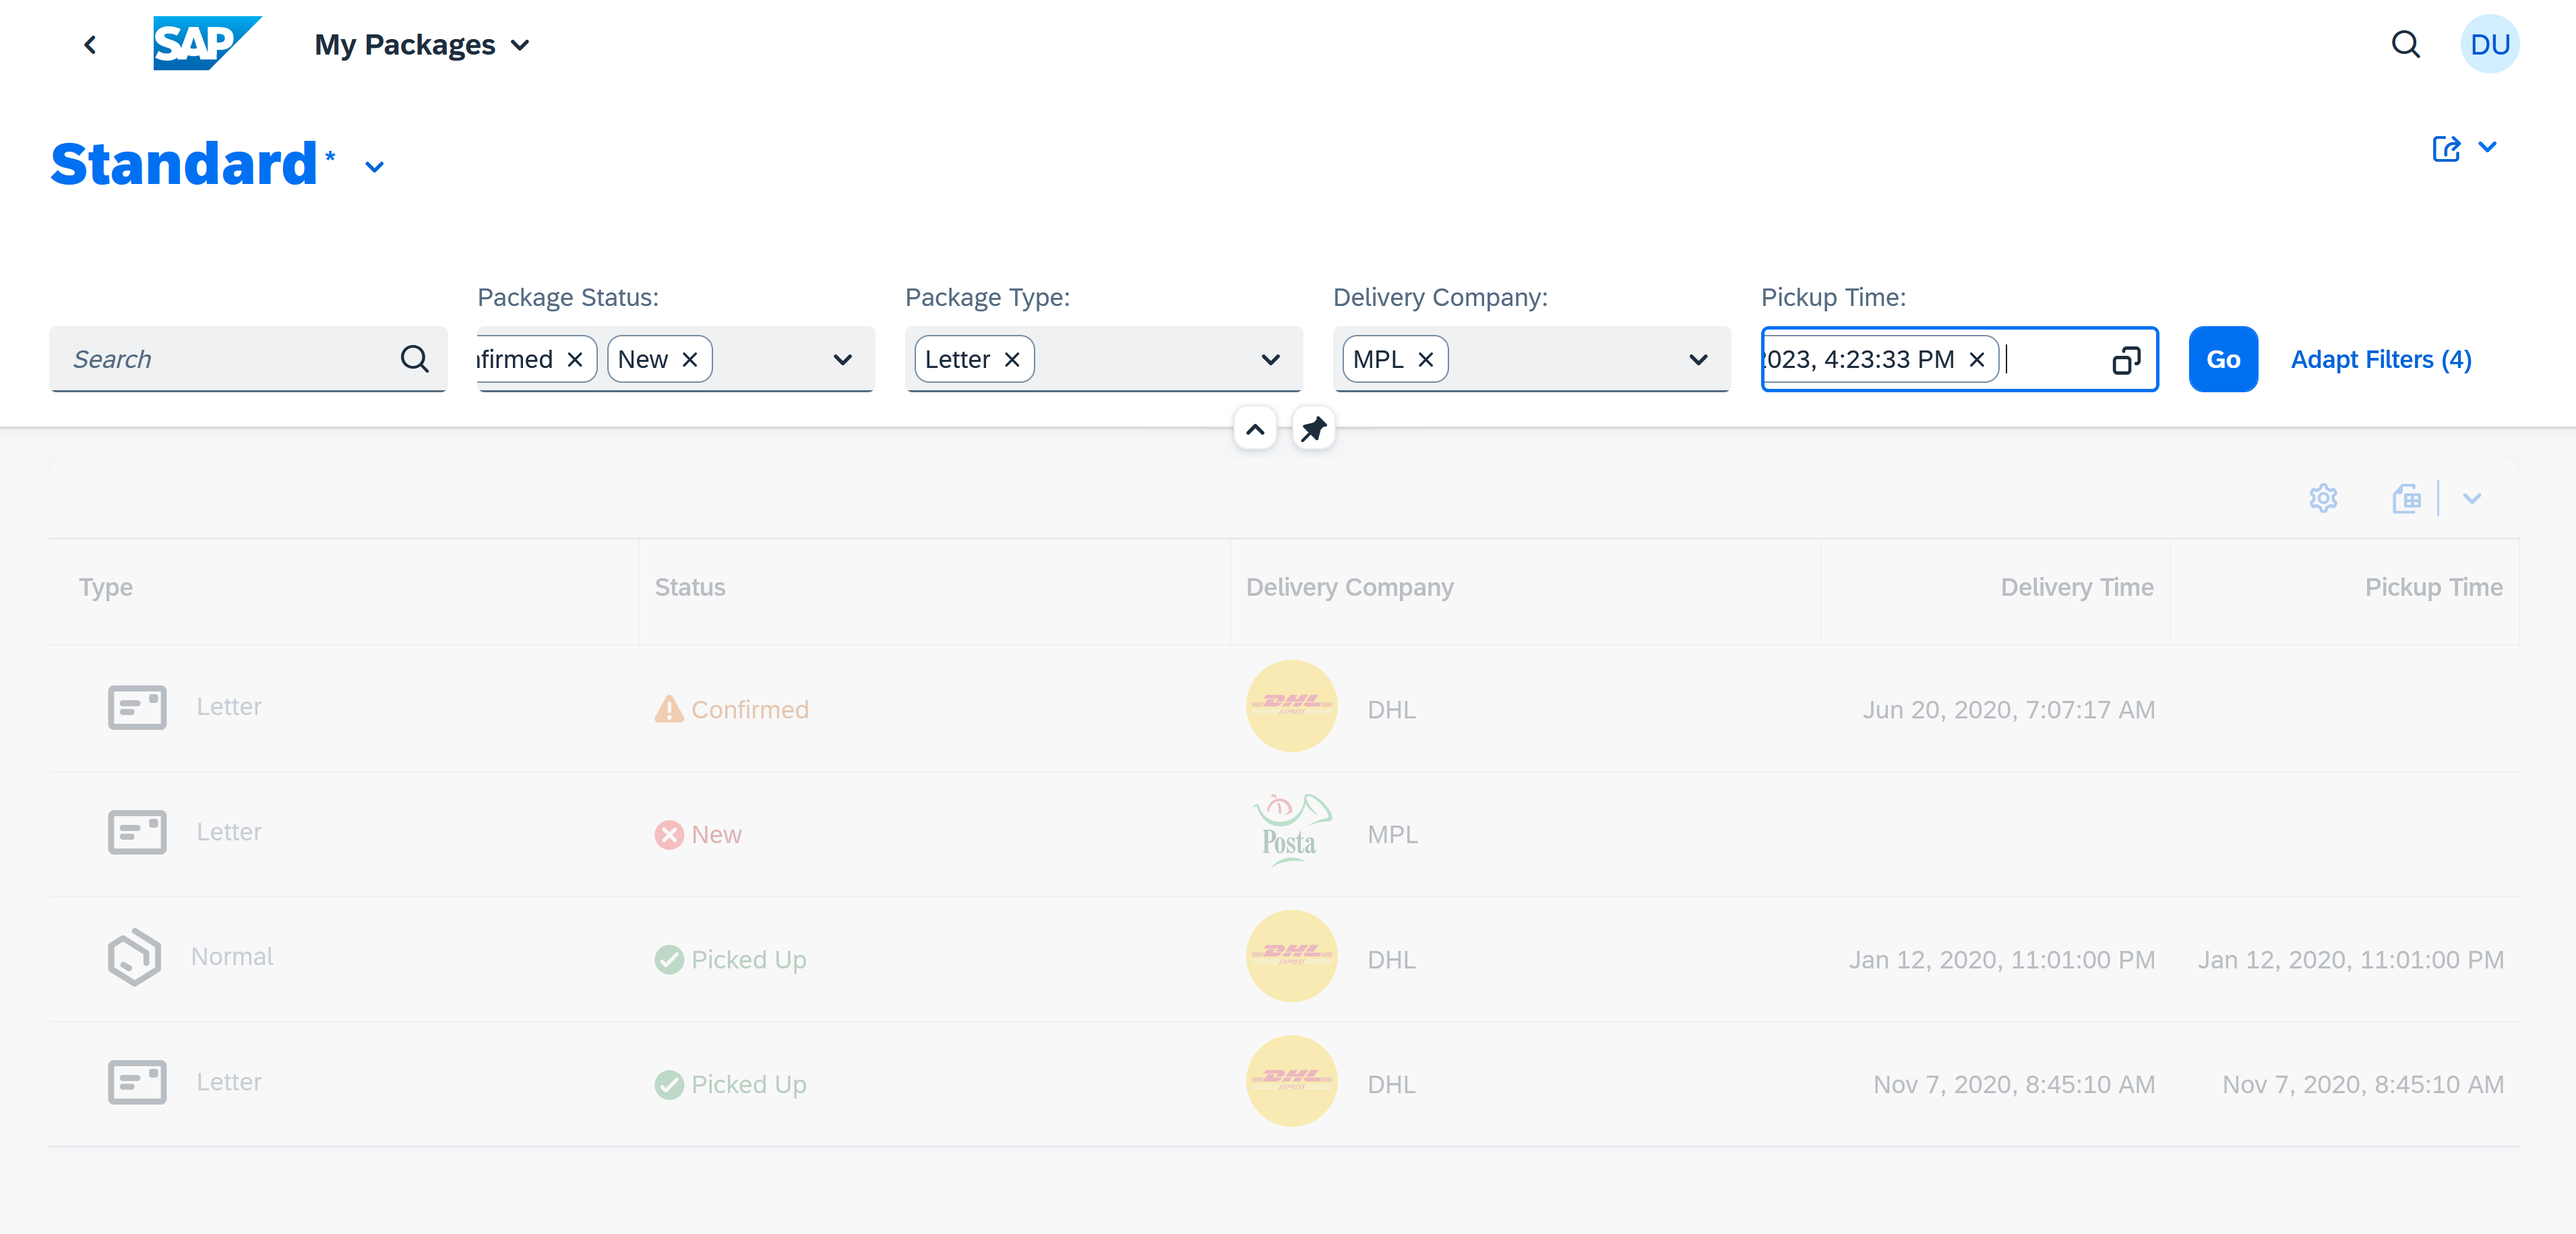
\includegraphics[width=0.75\linewidth]{images/user_doc/myPack/filterAdaptionScreen.png}}
	\vspace{5pt}
 
	\subcaptionbox{Clicked "Go"}{
		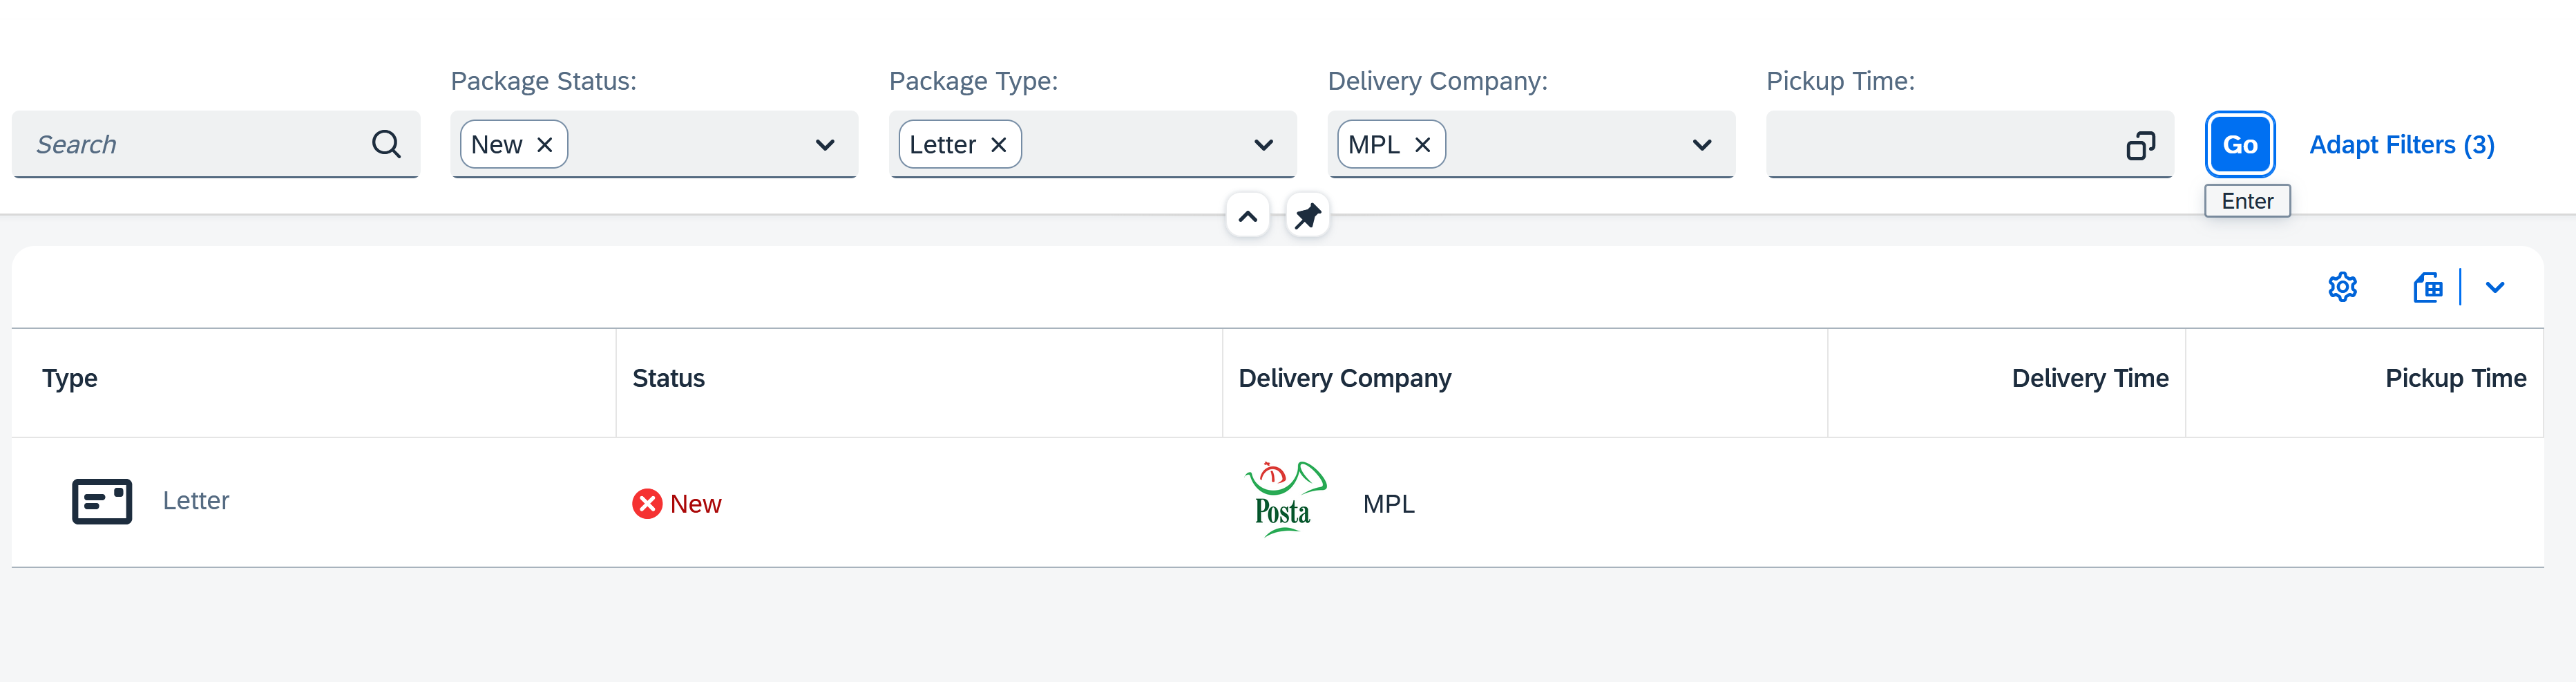
\includegraphics[width=0.85\linewidth]{images/user_doc/myPack/FilterDoneScreen.png}}
    \caption{My Package Home Screen - Adjust Filters}
    \label{fig:PHAjustFilters-2}
\end{figure}

\begin{figure}[H]
	\centering
	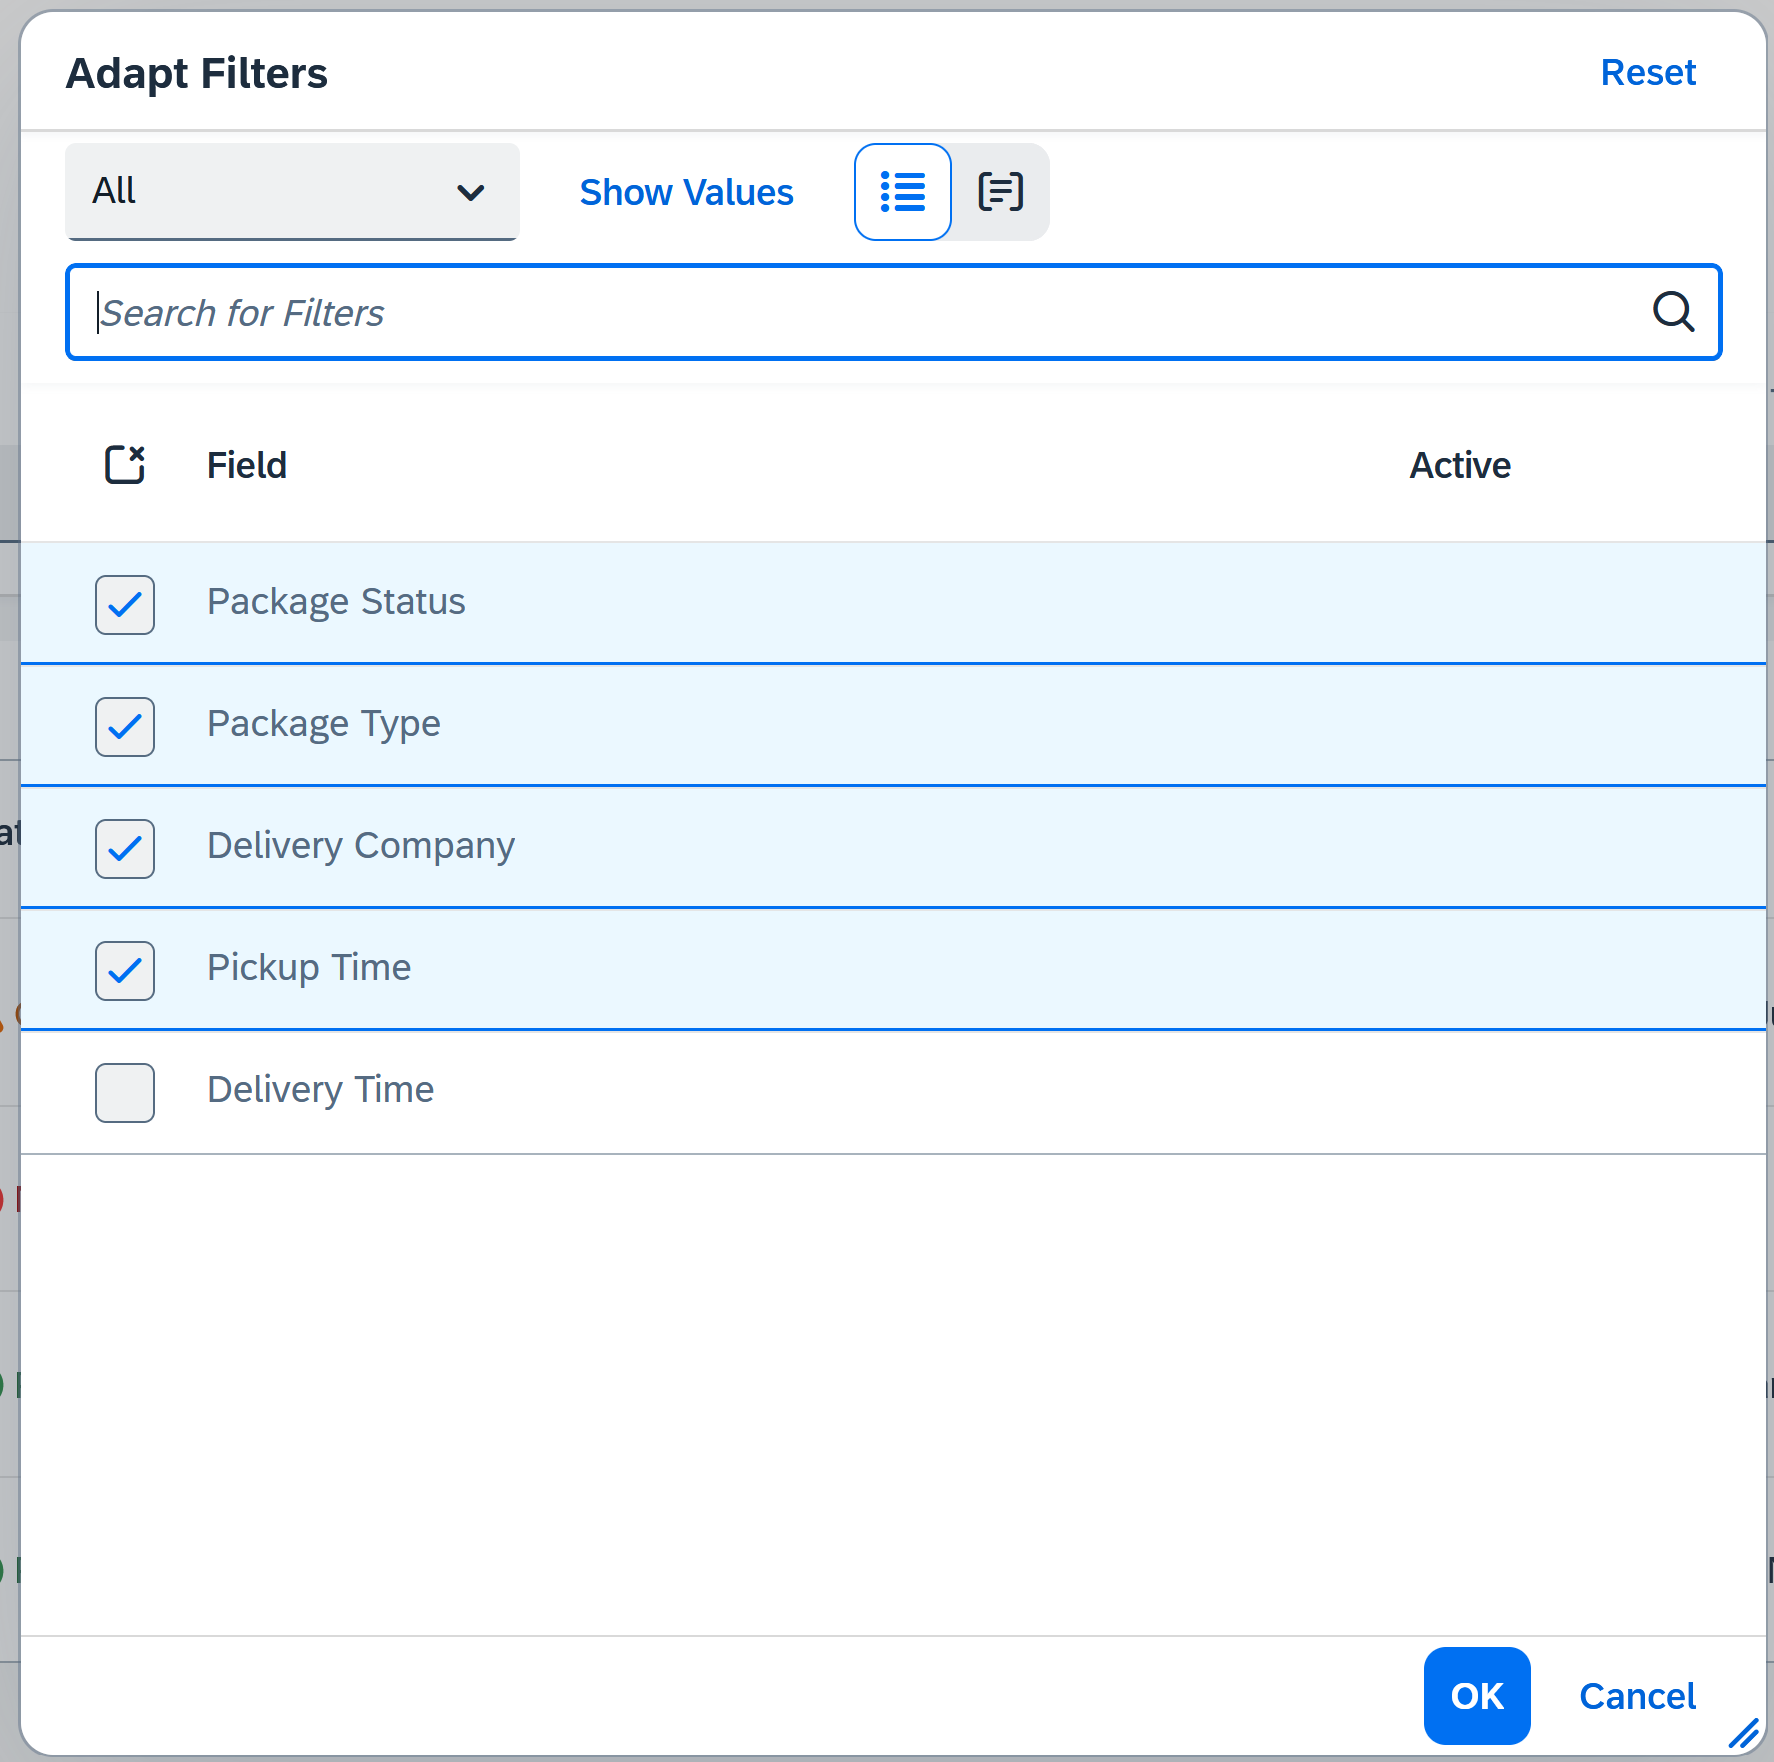
\includegraphics[height=200pt]{images/user_doc/myPack/MoreFIlterOption.png}
	\caption{My Package Filter Adaption Dialog - More Filters}
	\label{fig:mpMOreFilterAdaption}
\end{figure}
% ----------------------- Package Pickup ----------------------------
% 
%  ---------------------------------------------------------------

\subsection{Package Pickup}
\label{subsec:pp}

The \textbf{Package Pickup} application is used by the \textbf{End User} to pick up any personal confirmed parcels (registered at the reception and confirmed with a storage slot). The reader can navigate to \autoref{subsec:dev-ui-pp} for more implementation details. 
The summarized main actions the \textbf{End User} (see \autoref{sec:UdocEndUser} for all related applications) can take within the application are listed here:
\begin{compactenum}
	\item Browse the owned packages that can be picked up.
    \item Pickup the listed owned packages.
\end{compactenum}

\noindent
\textbf{Hint}: The application supports users accessing it from mobile devices. In case an employee is unable to access his or her mobile at the moment of pickup, he or she should ask the receptionist to pickup the package for him or her.


\subsubsection{Home Screen - Selection}
After clicking on the application tile, an \textbf{End User} is redirected to the 'Home Screen'. A list of packages is displayed, if there exists at least one package to pickup. 
The list displays \textbf{the type with icon}, \textbf{the delivery company}, \textbf{the registration time} and \textbf{the location} of the packages (\autoref{fig:PickupHomeScreen-1}/a). 
If no package exists to pickup, a no package message is shown. 
The total number of packages that can be pickup can be found at the title of the package list (\autoref{fig:PickupHomeScreen-1}/b).

In case there are existing packages, one or multiple packages can be selected from the list to pickup. 
The "Toggle All" selection box can also be used to select or deselect all packages at once (\autoref{fig:PickupHomeScreen-2}). 

\begin{figure}[H]
	\centering
	\subcaptionbox{Home Screen with Packages}{
		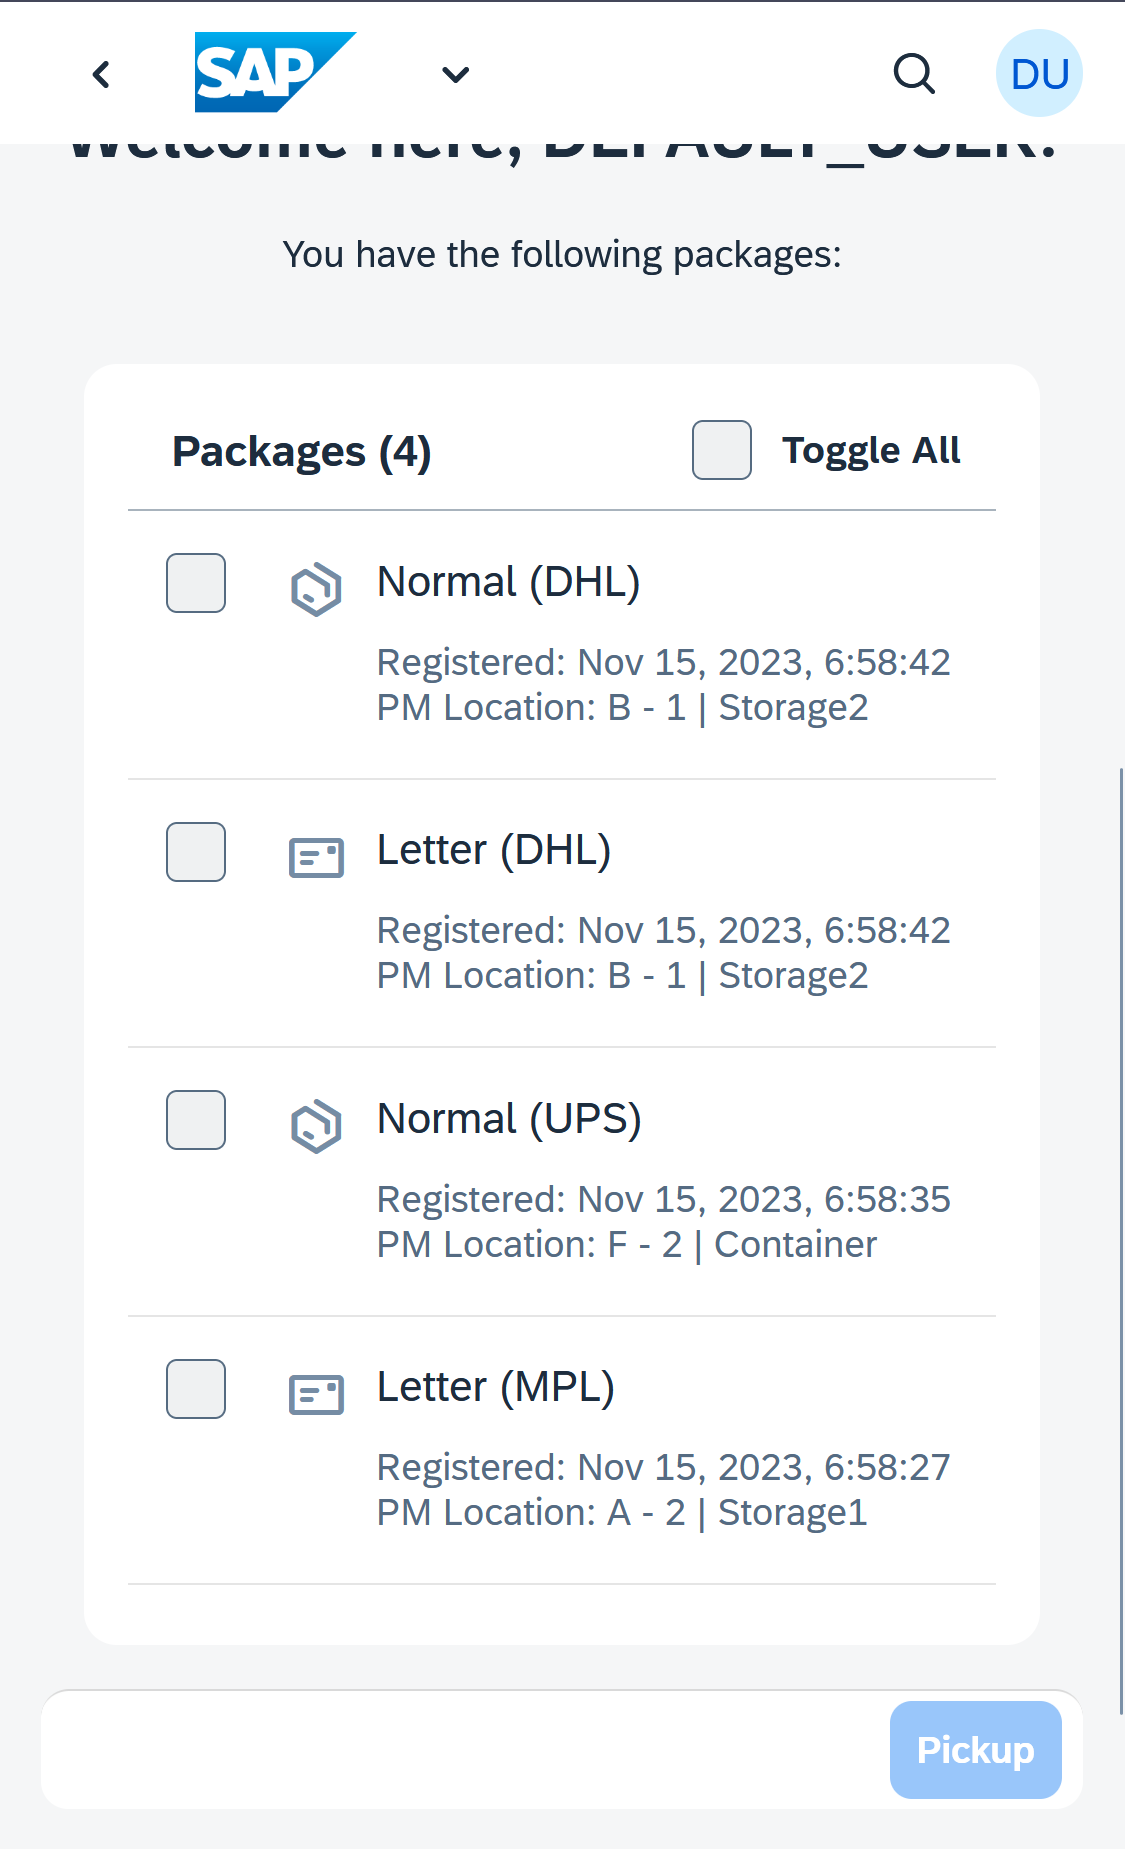
\includegraphics[width=0.39\linewidth]{images/user_doc/pickup/HomeScreenList.png}}
	\hspace{8pt}
	\subcaptionbox{Home Screen without Packages}{
		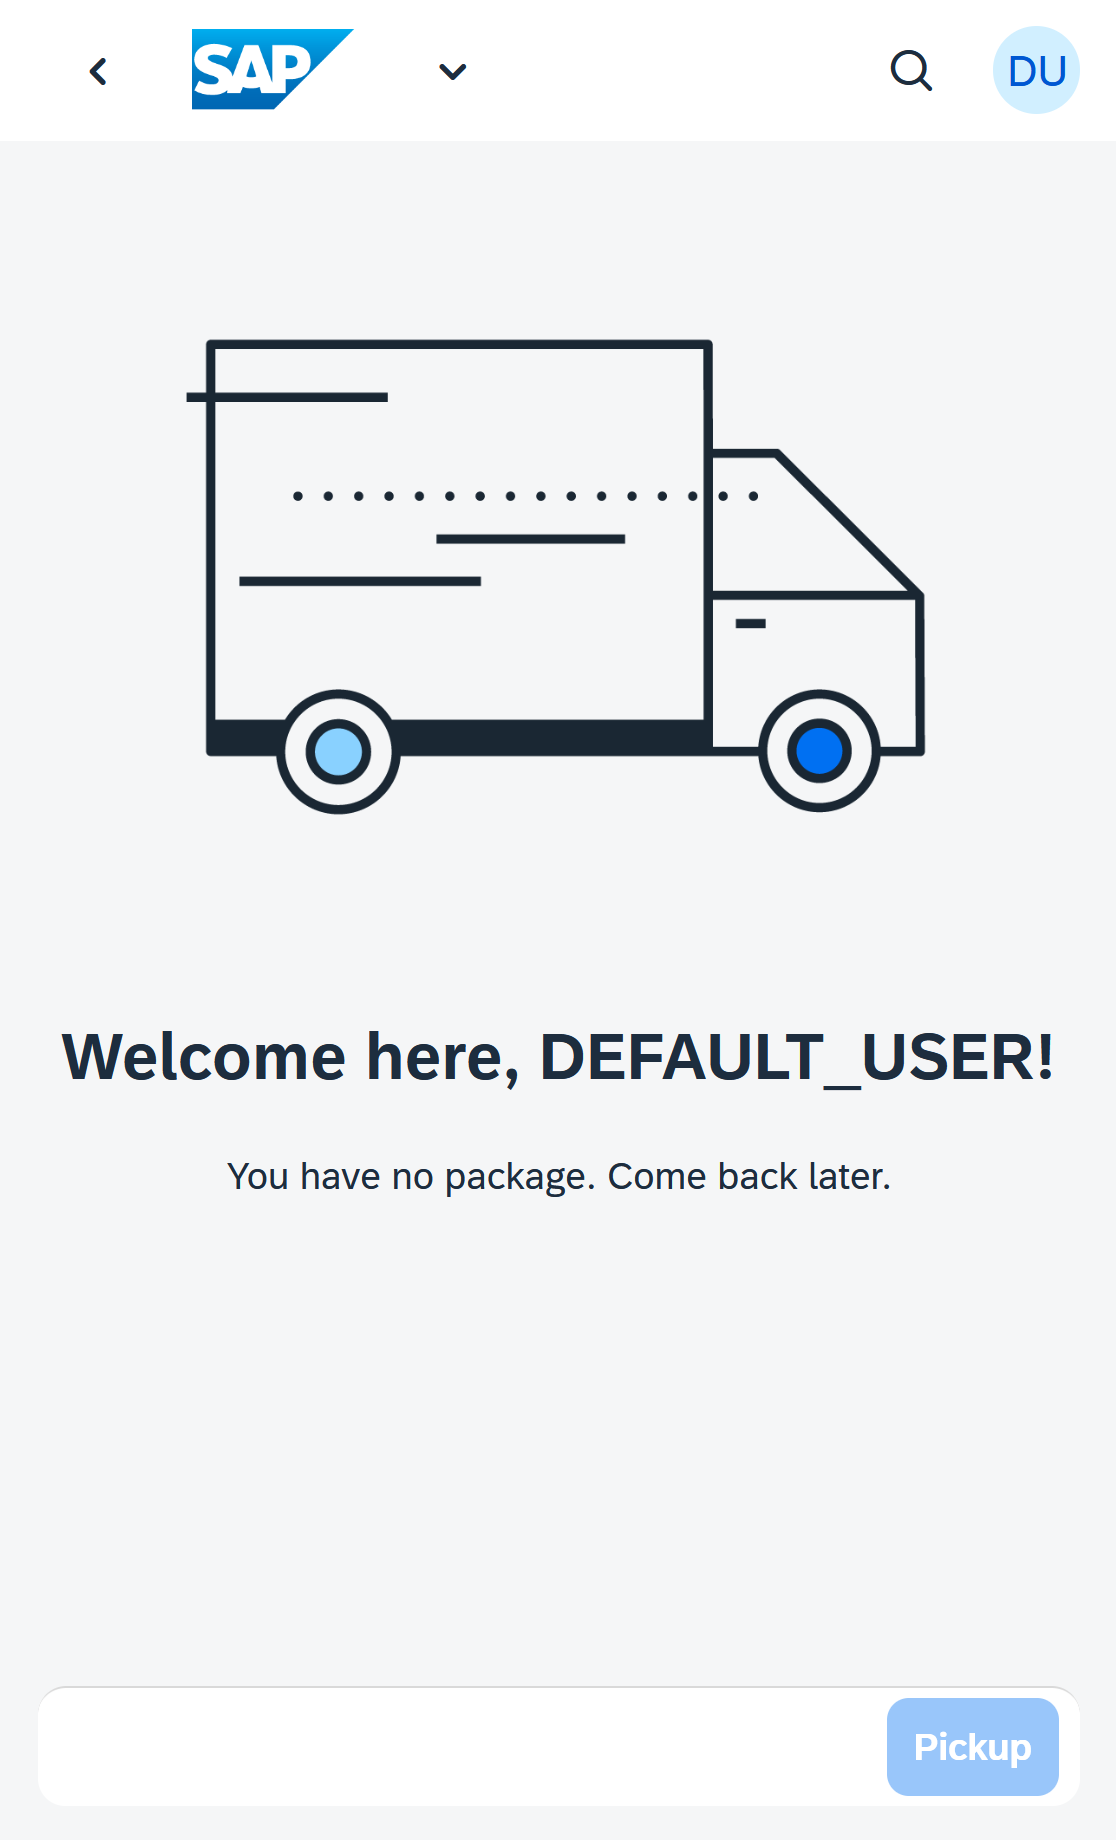
\includegraphics[width=0.39\linewidth]{images/user_doc/pickup/HomeScreenNoPackage.png}}
	\caption{Pickup Home Screen - Package Existence Guide}
	\label{fig:PickupHomeScreen-1}
\end{figure}

\begin{figure}[H]
	\centering
	\subcaptionbox{Home Screen Single Selection}{
		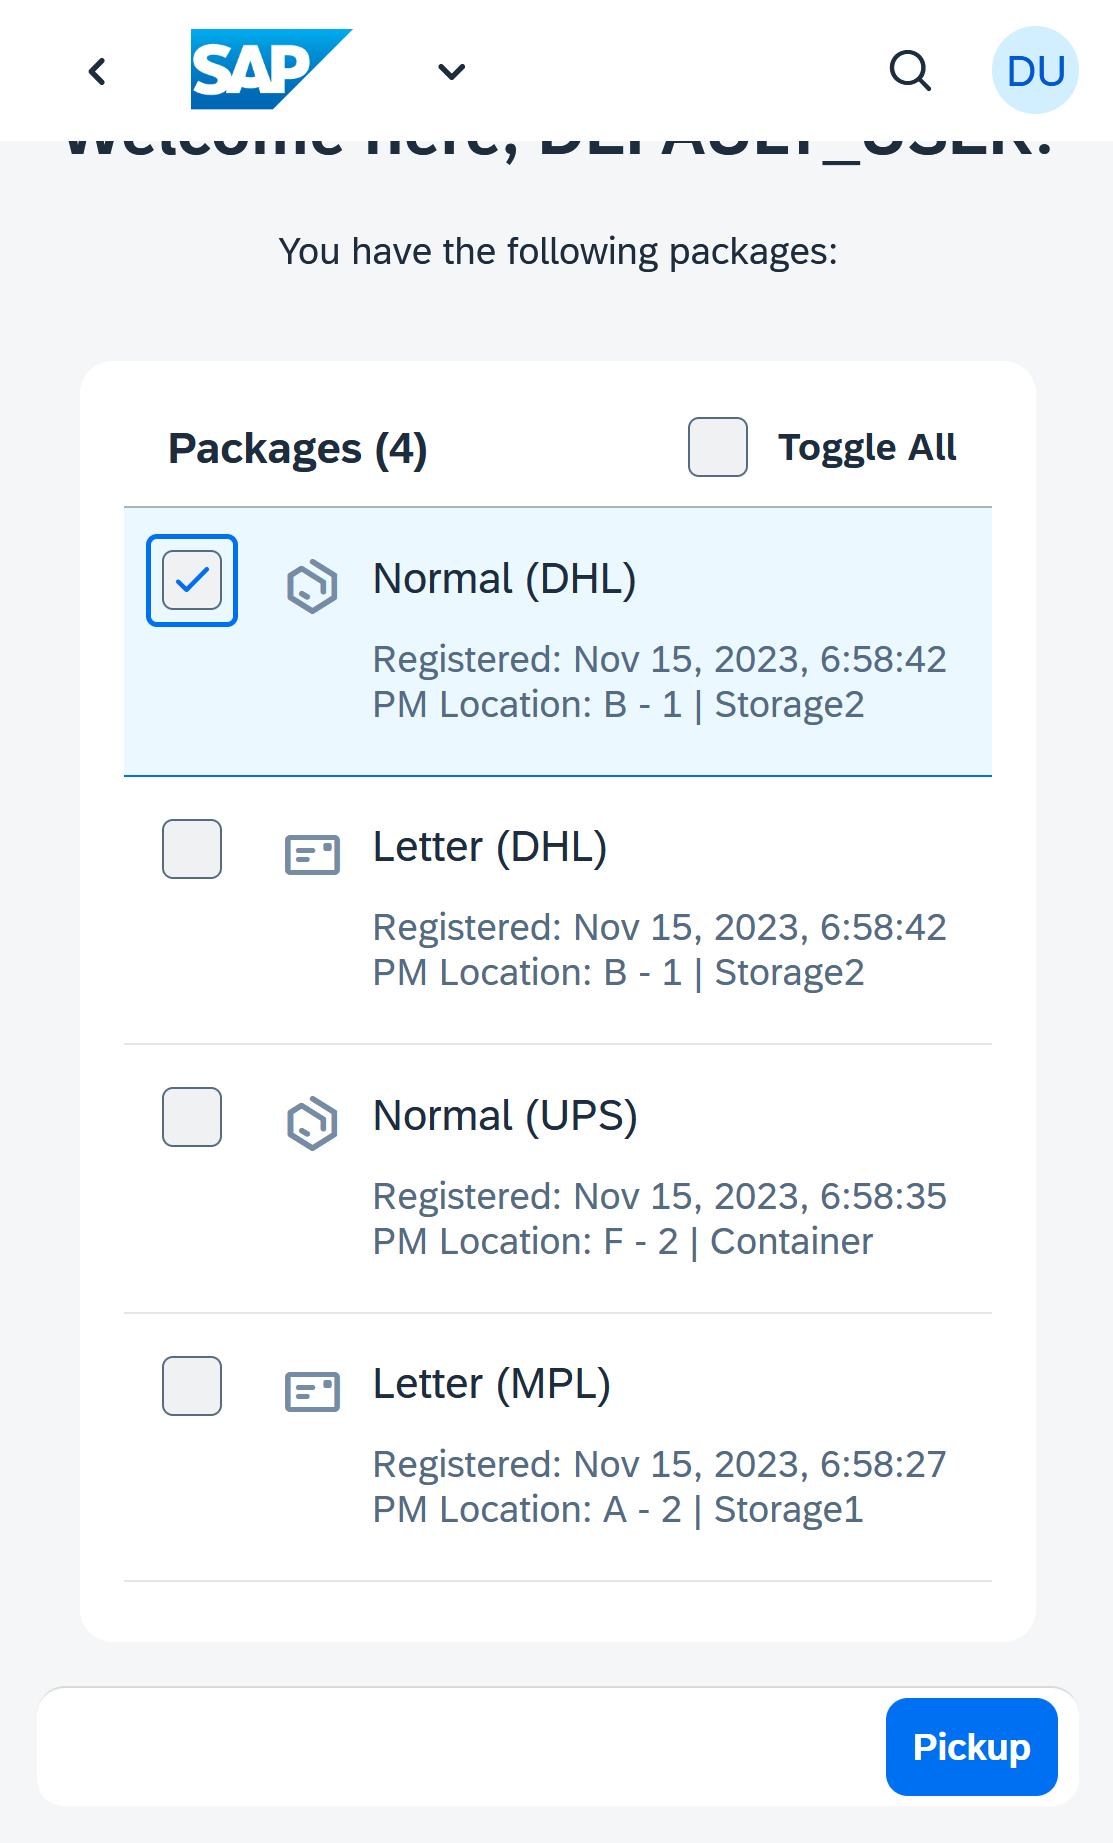
\includegraphics[width=0.45\linewidth]{images/user_doc/pickup/HomeScreenSelectOne.png}}
	\hspace{5pt}
	\subcaptionbox{Home Screen Multiple Selection}{
		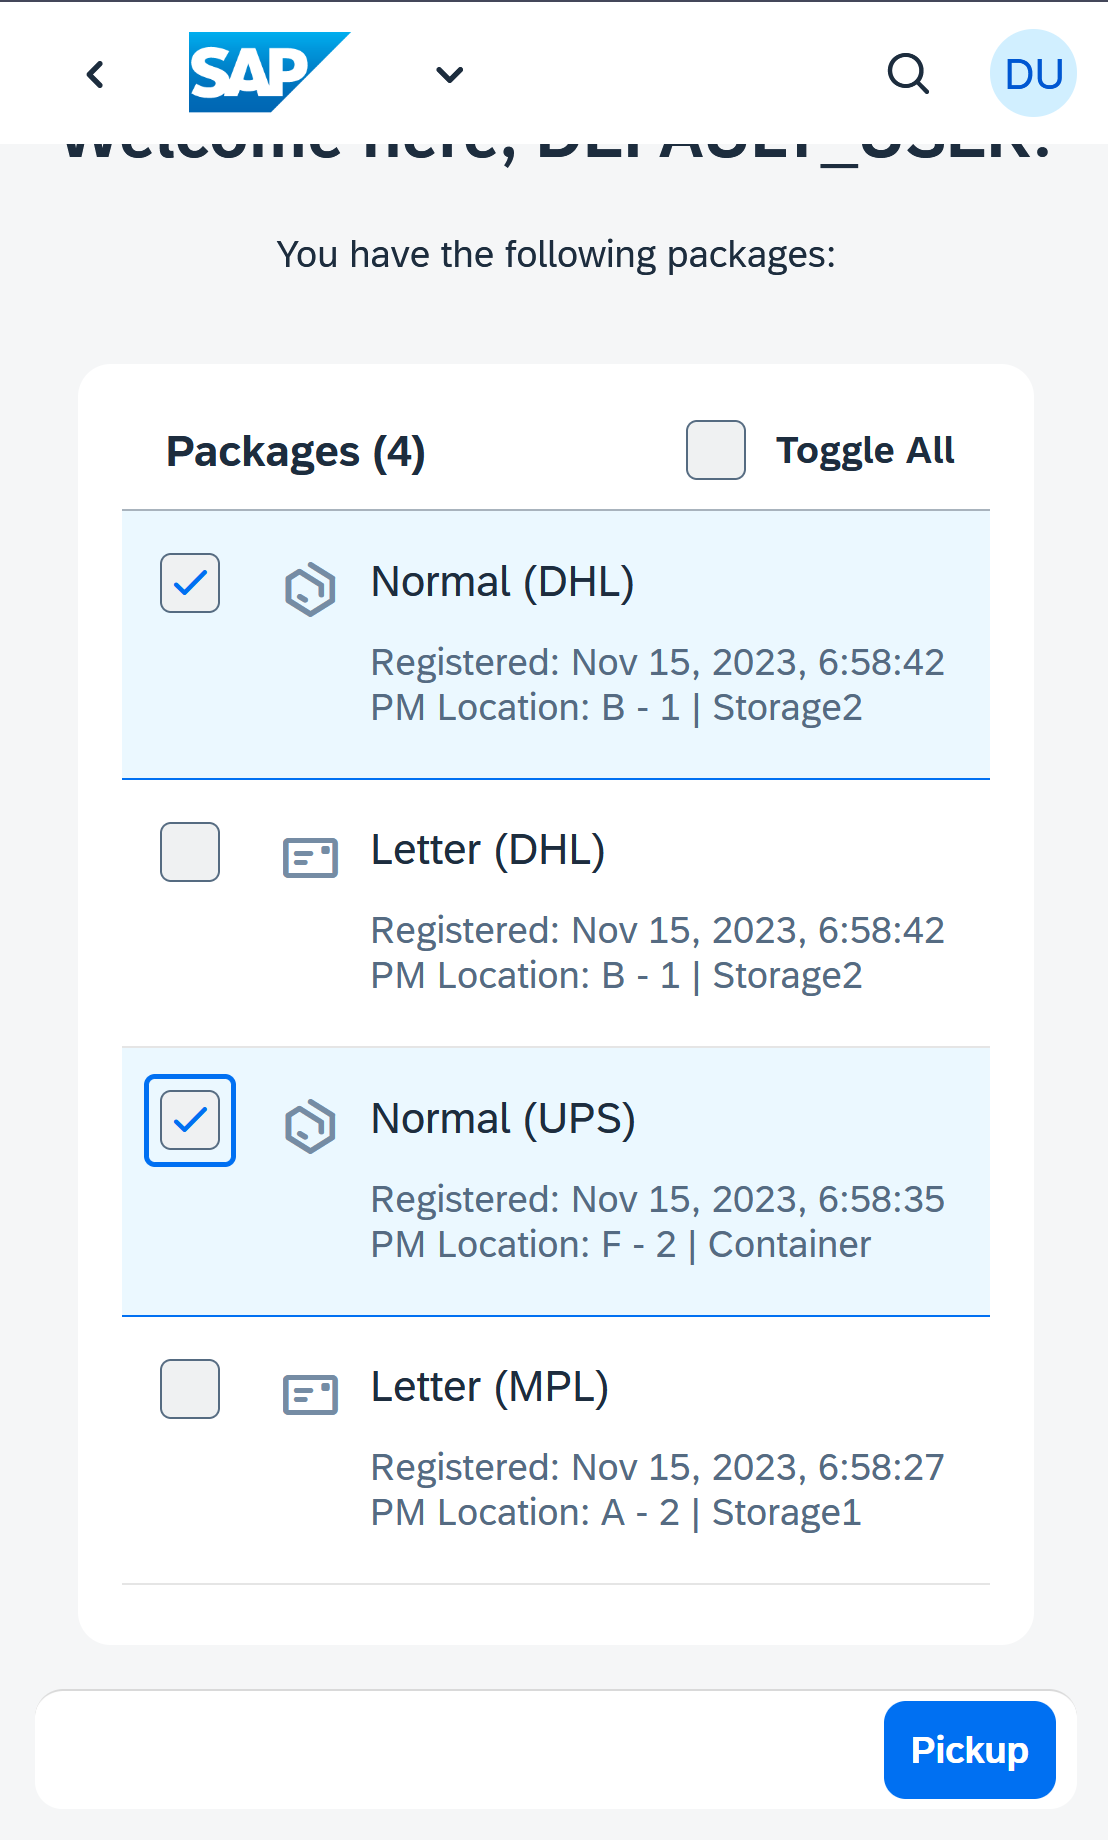
\includegraphics[width=0.45\linewidth]{images/user_doc/pickup/HomeScreenMultiSelect.png}}

    \subcaptionbox{Home Screen Select All}{
		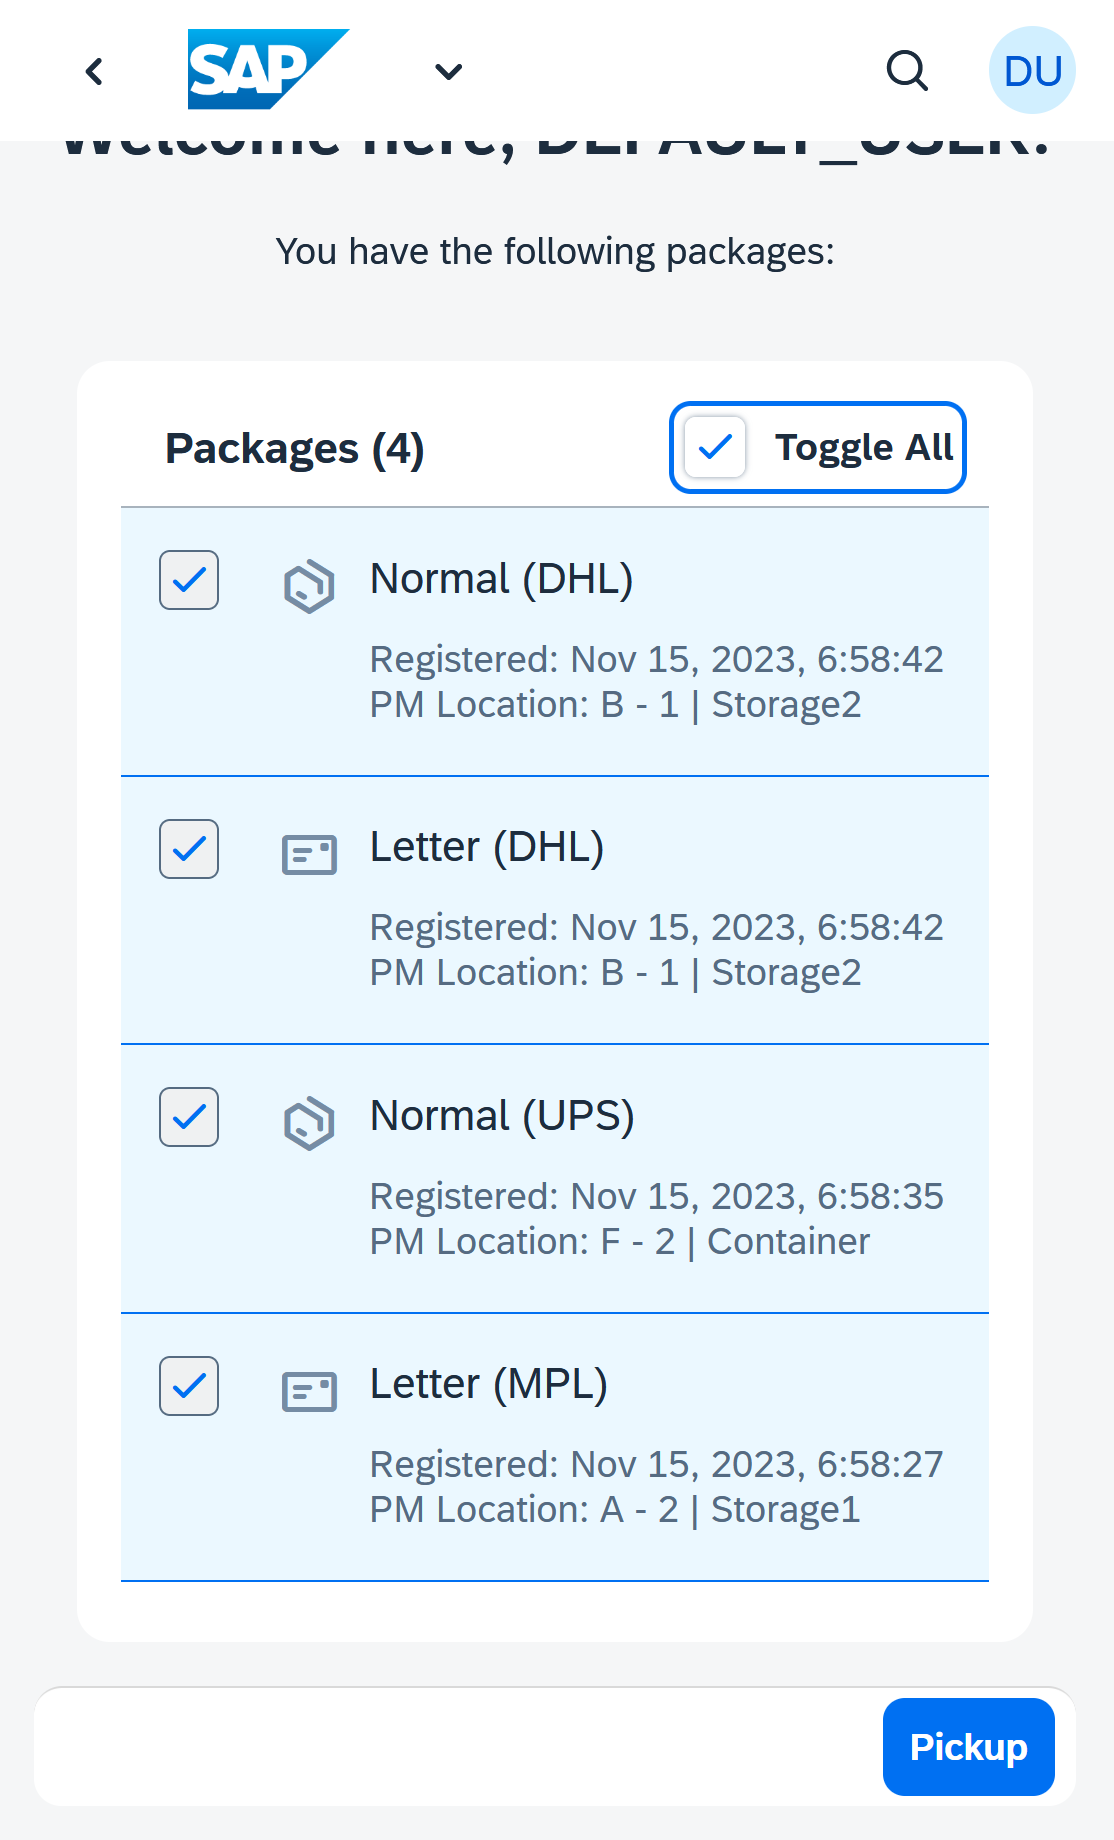
\includegraphics[width=0.45\linewidth]{images/user_doc/pickup/HomeScreenToggleAll.png}}
	\hspace{5pt}
	\subcaptionbox{Home Screen Deselect All}{
		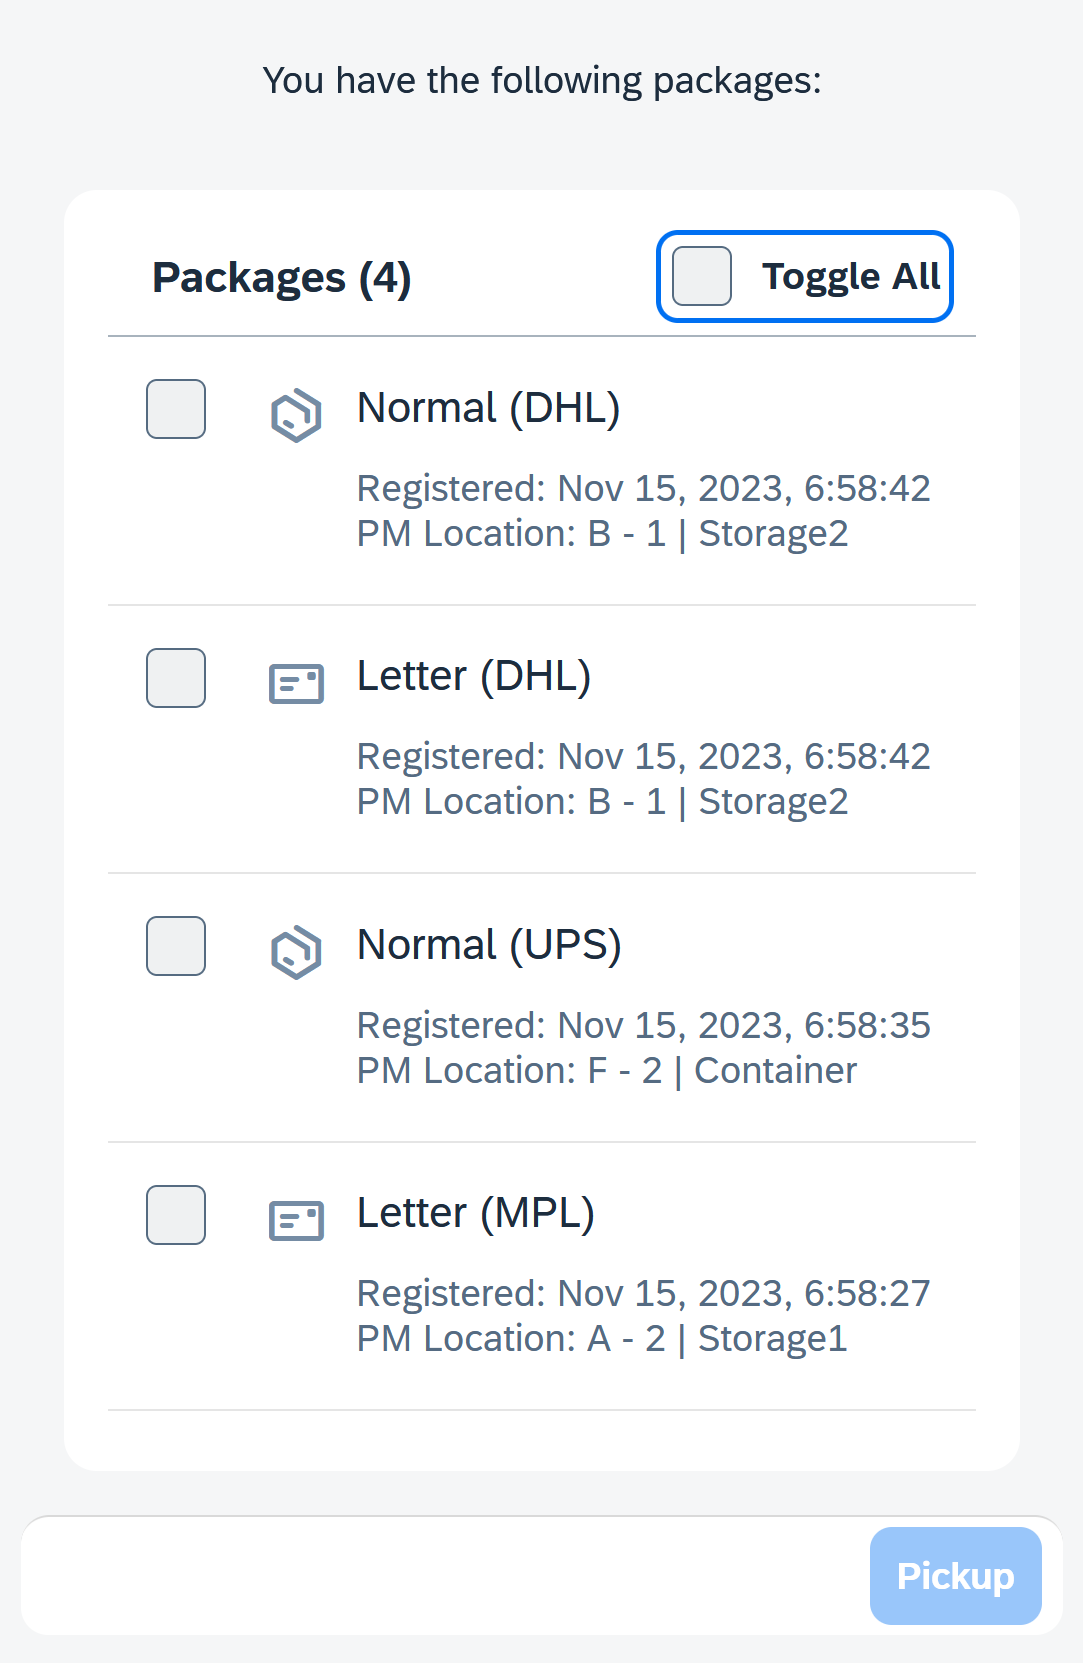
\includegraphics[width=0.45\linewidth]{images/user_doc/pickup/HomeScreenDeToggleAll.png}}
	\caption{Pickup Home Screen - Package Selection Guide}
	\label{fig:PickupHomeScreen-2}
\end{figure}


\subsubsection{Home Screen - Pickup}
The "Pickup" button at right bottom corner will only be enabled if at least one package is selected. In case it is enabled, the user can pick up the selected packages by left clicking the "Pickup" button, which will trigger a confirmation dialog (\autoref{fig:PickupDialog}). 

If "Cancel" is chosen, the dialog closes and no modification is made. If "OK" is chosen, all packages selected will be marked as pickup, removed from the list and the user will be navigated to the "Done Screen". At this point, the process of the picked up package will be closed, the package data will never be deleted and \textbf{My Packages} application (\autoref{subsec:ph}) can be used to check the package history.

\bigskip
\begin{figure}[H]
	\centering
	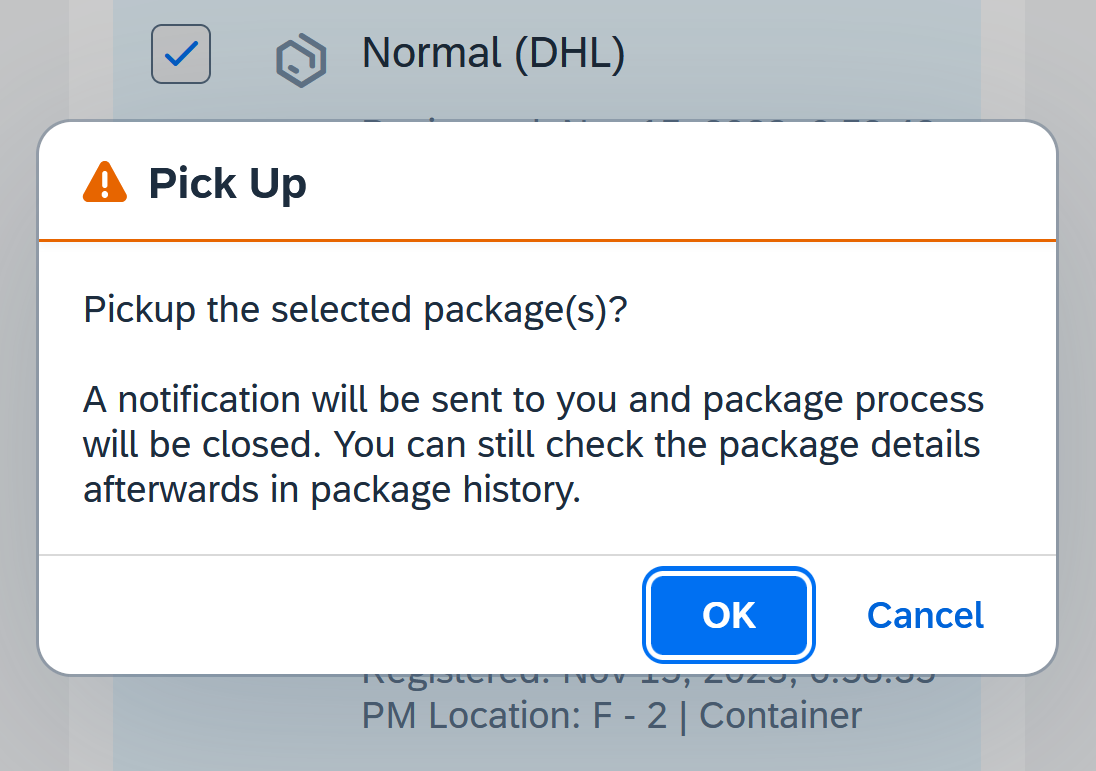
\includegraphics[height=250pt]{images/user_doc/pickup/PickupDialog.png}
	\caption{Pickup Home Screen - Pickup Dialog}
	\label{fig:PickupDialog}
\end{figure}


\subsubsection{Done Screen}

At the "Done Screen", if the \textbf{End User} have more packages to pickup, a list of packages will be displayed showing their \textbf{type with icon}, \textbf{delivery company} and \textbf{location info}. Otherwise, a no more packages message is shown (figure \ref{fig:PickupDoneScreen-1}). 

By left clicking on "Close" button at the right lower corner of the page, the user is navigated back to "Home Screen".
From there, a new pickup iteration may start.

\begin{figure}[H]
	\centering
	\subcaptionbox{Done Screen with Packages}{
		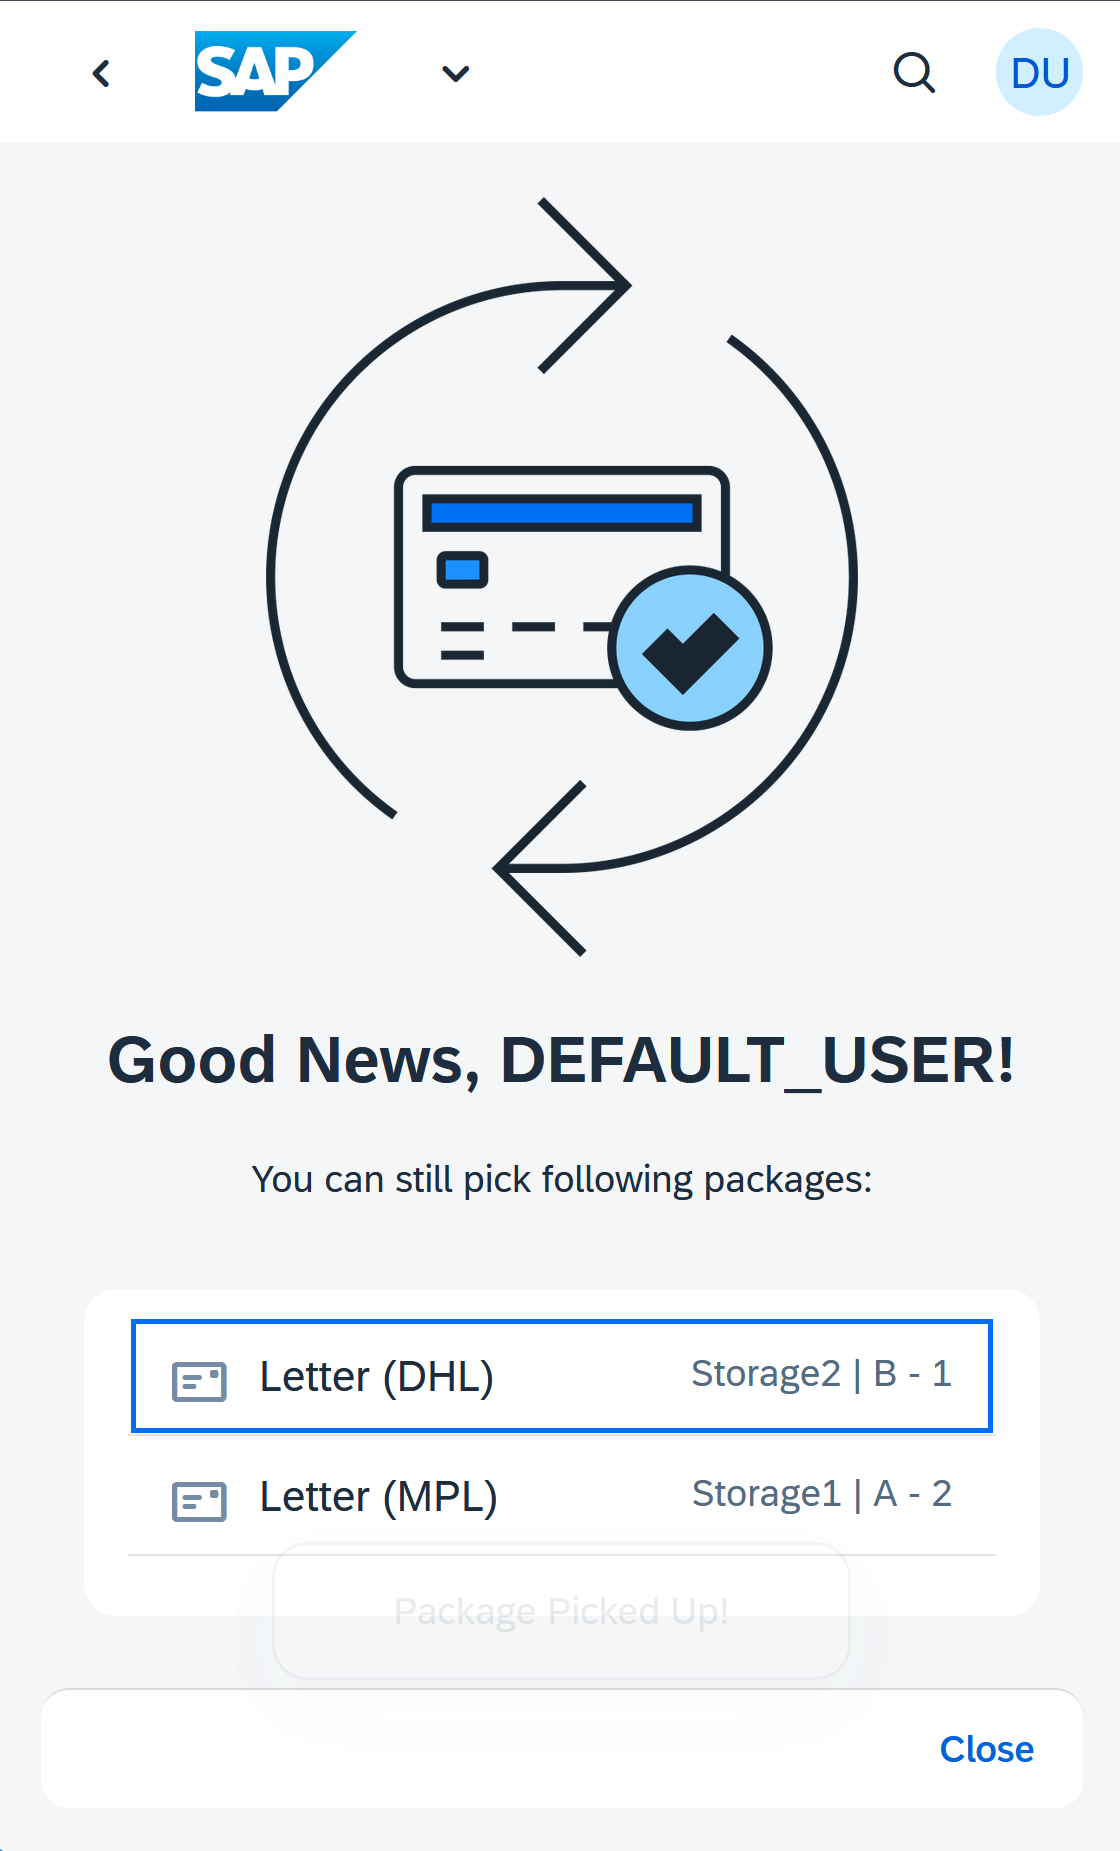
\includegraphics[width=0.45\linewidth]{images/user_doc/pickup/DoneScreenRemainPackages.png}}
	\hspace{5pt}
	\subcaptionbox{Done Screen without Packages}{
		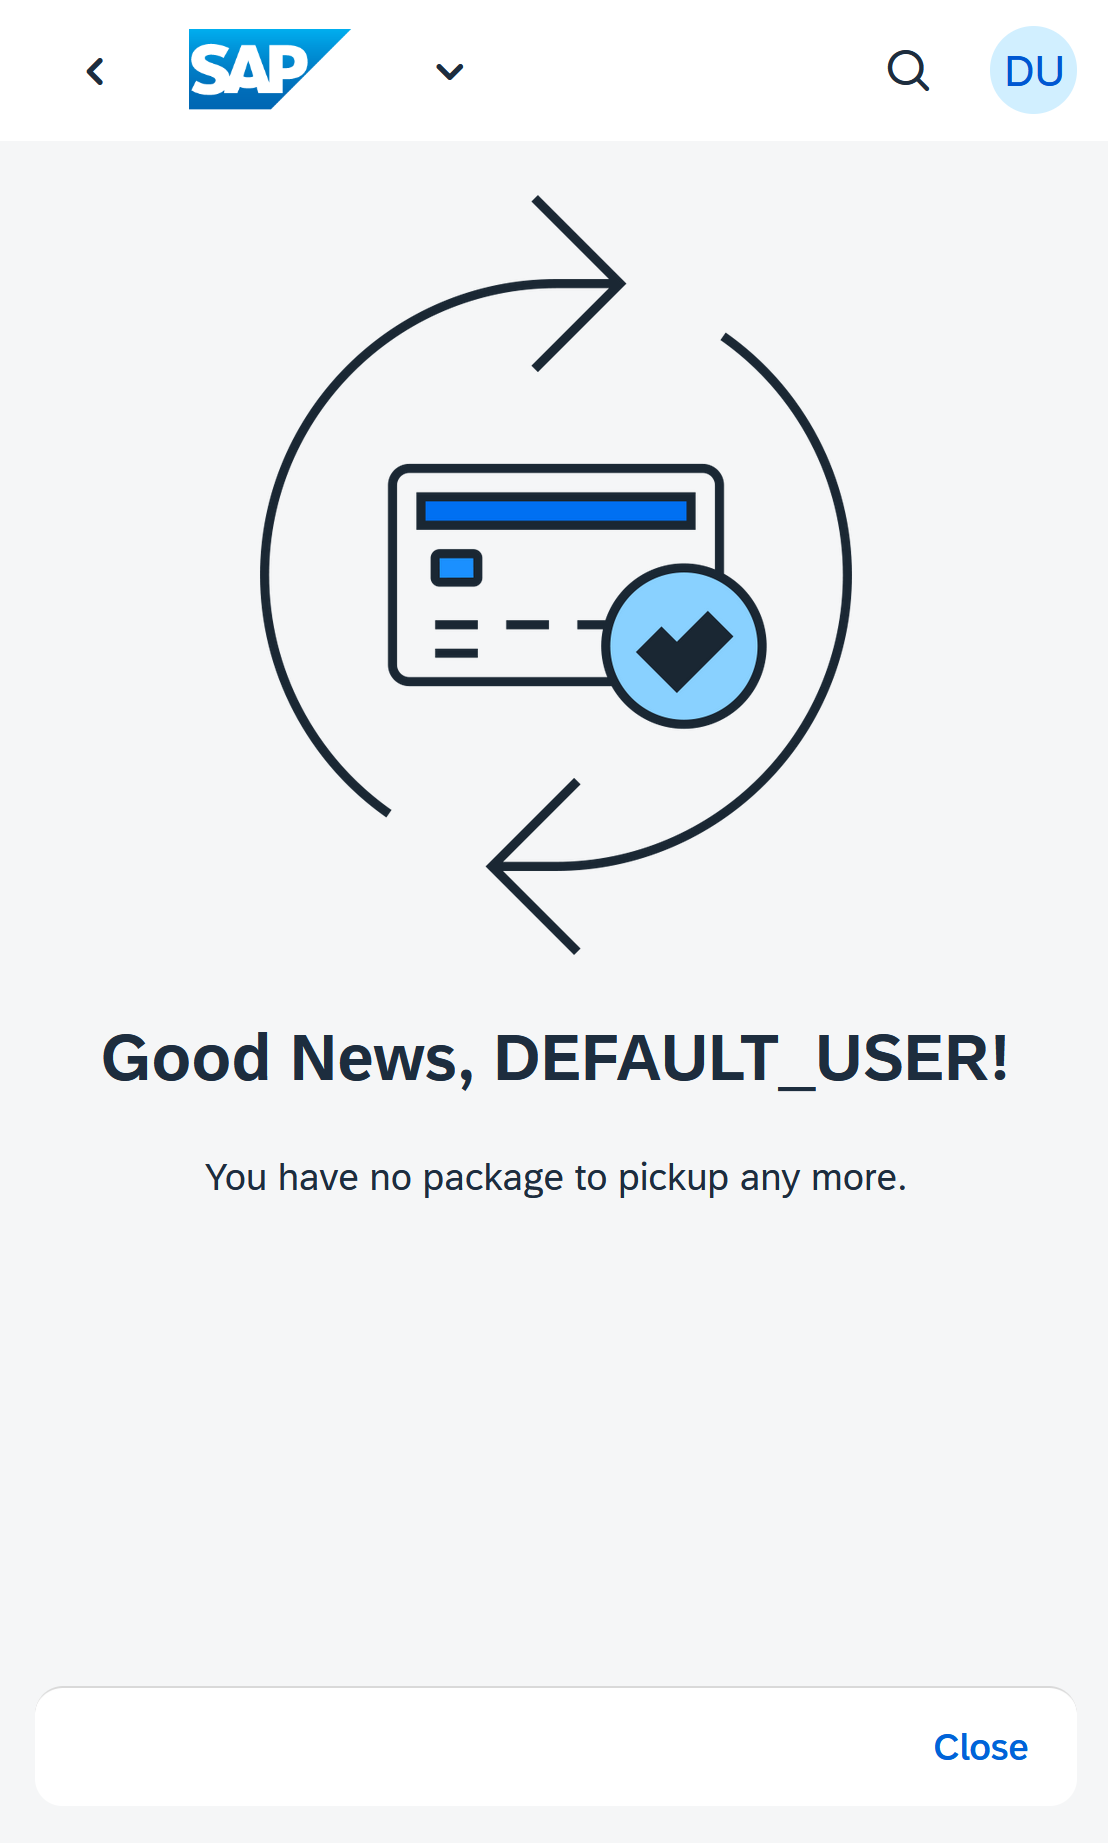
\includegraphics[width=0.45\linewidth]{images/user_doc/pickup/DoneScreenNoPackage.png}}
	\caption{Pickup Done Screen - Package Existence Guide}
	\label{fig:PickupDoneScreen-1}
\end{figure}

%\pagebreak

\section{Receptionist}
\label{sec:UdocReceptionist}

A \textbf{Receptionist} (see \autoref{sec:GeneralRequisite} for all possible roles) is granted the access to the two applications under the \textbf{Parcel Handling} section, namely \textbf{Register Packages} (\autoref{subsec:rp}) and \textbf{Manage Packages} (\autoref{subsec:mp}). A receptionist can quick jump to the section by left clicking the "Parcel Handling" tab. A receptionist can enter the application by left clicking the tiles (\autoref{fig:PHApplications}).

\begin{figure}[htb!]
	\centering
	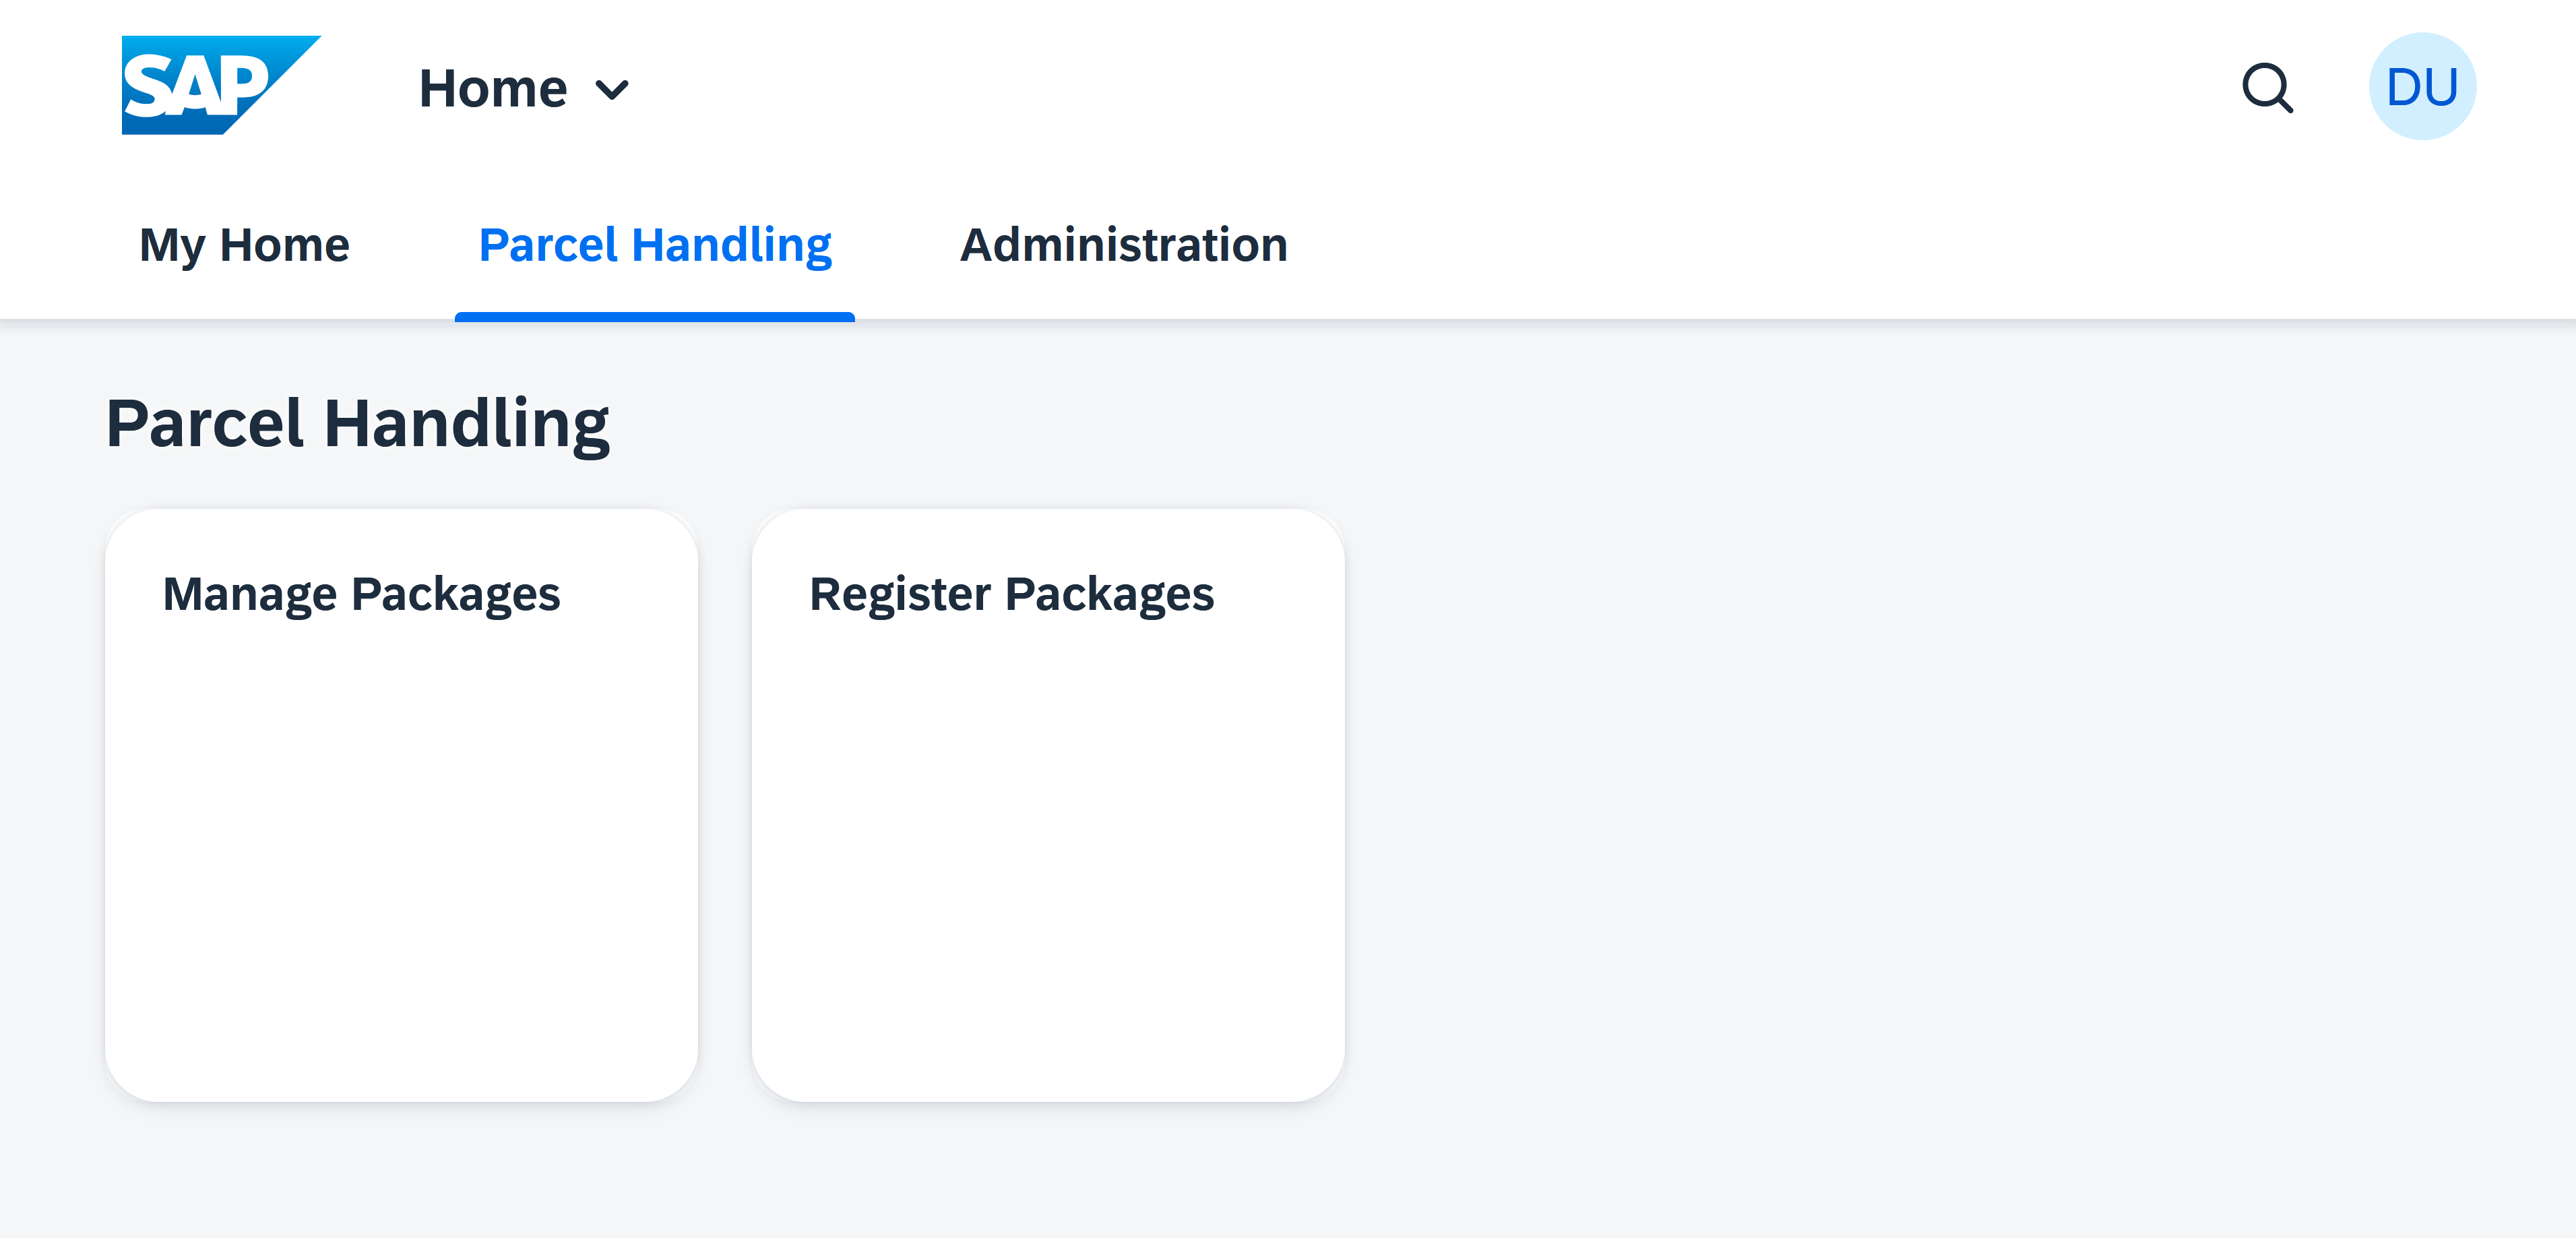
\includegraphics[width=0.85\linewidth]{images/user_doc/overviews/ParcelHandlingTab.png}
	\caption{Parcel Handling Applications}
	\label{fig:PHApplications}
\end{figure}


\subsection{Register Packages}
\label{subsec:rp}

When the delivery person arrived at the reception with the new parcels, \textbf{Register Packages} application should be used by the \textbf{Receptionist} to register the newly arrived parcels into the system (see \autoref{sec:UdocReceptionist} for all receptionist related applications). After the registration, \textbf{Receptionist} will be automatically redirected to \textbf{Manage Packages}. The reader can navigate to \autoref{subsec:dev-ui-rp} for more implementation details. 
The summarized main actions the \textbf{Receptionist} can take within the application are listed here:

\begin{compactenum}
	\item Register a newly arrived package.
    \item Register multiple newly arrived packages.
    \item Discard current registration.
\end{compactenum}

\subsubsection{Data Entry}

When the \textbf{Receptionist} clicks on the \textbf{Register Packages} application tile, he or she is redirected to the main screen, the 'Package Registration Form' (see \autoref{fig:RPOverview}). At this point, \textbf{Recipient}, \textbf{Type} (package type), \textbf{Receptionist}, \textbf{Delivery Company} and optionally \textbf{Comment} of the package are required by the form (\autoref{fig:RPformEntry}).

\begin{figure}[htb!]
	\centering
	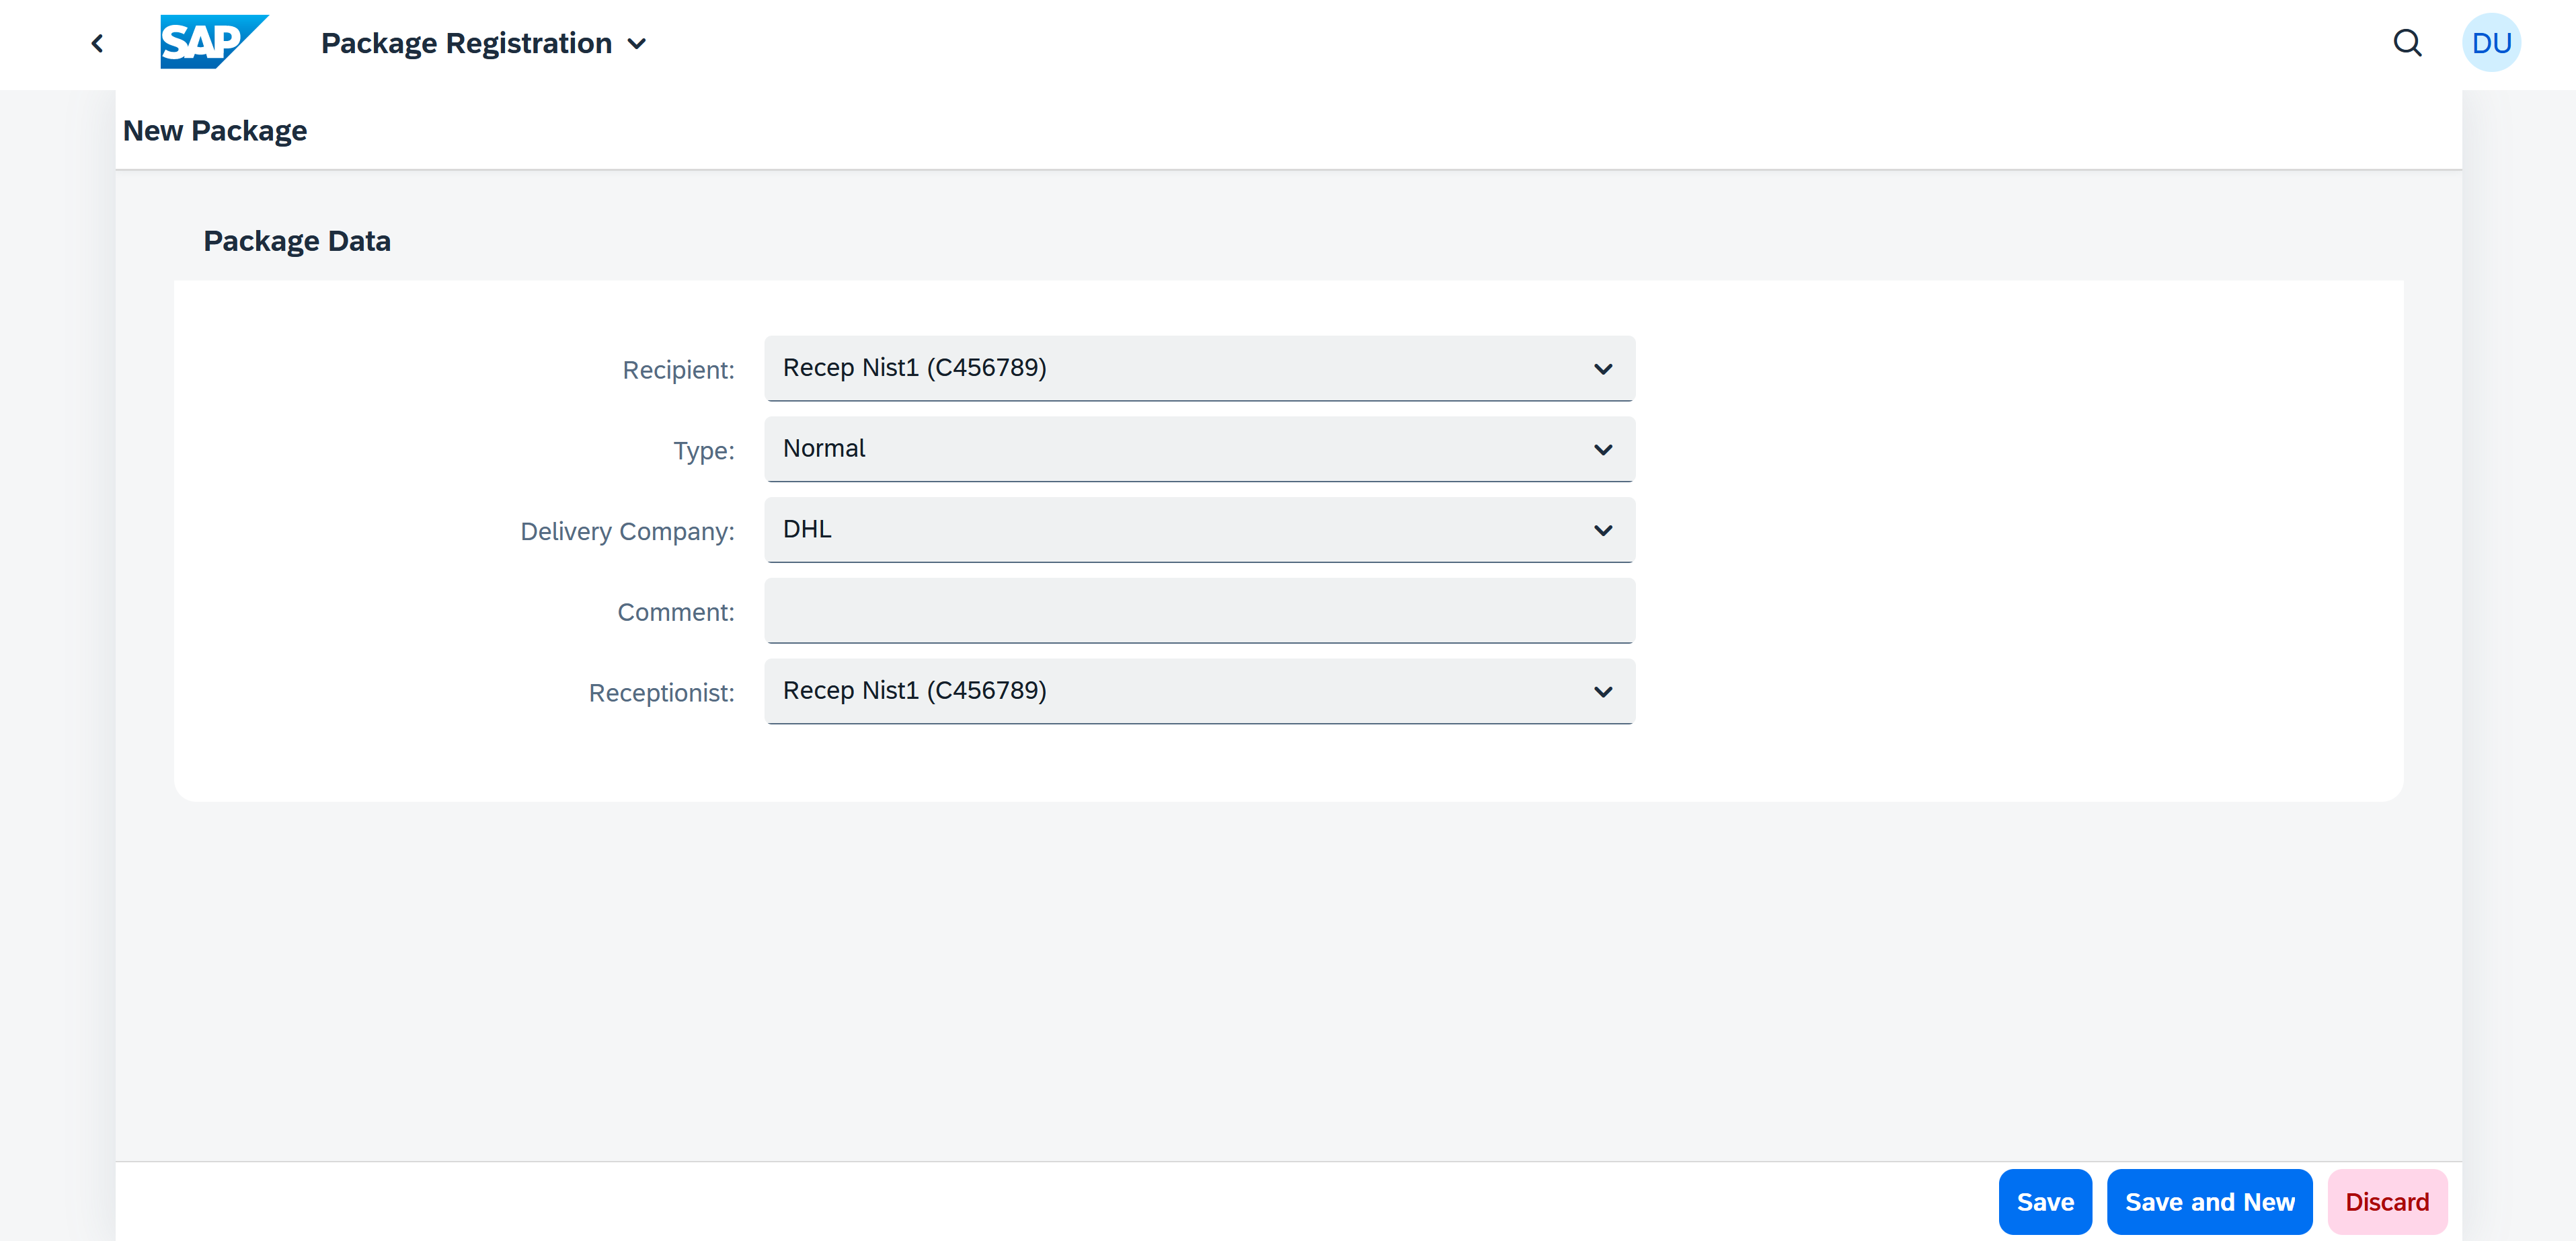
\includegraphics[width=0.95\linewidth]{images/user_doc/registration/overview.png}
	\caption{Package Registration Form}
	\label{fig:RPOverview}
\end{figure}


\begin{figure}[htb!]
	\centering
	\subcaptionbox{Step 1: Choose Recipient}{
		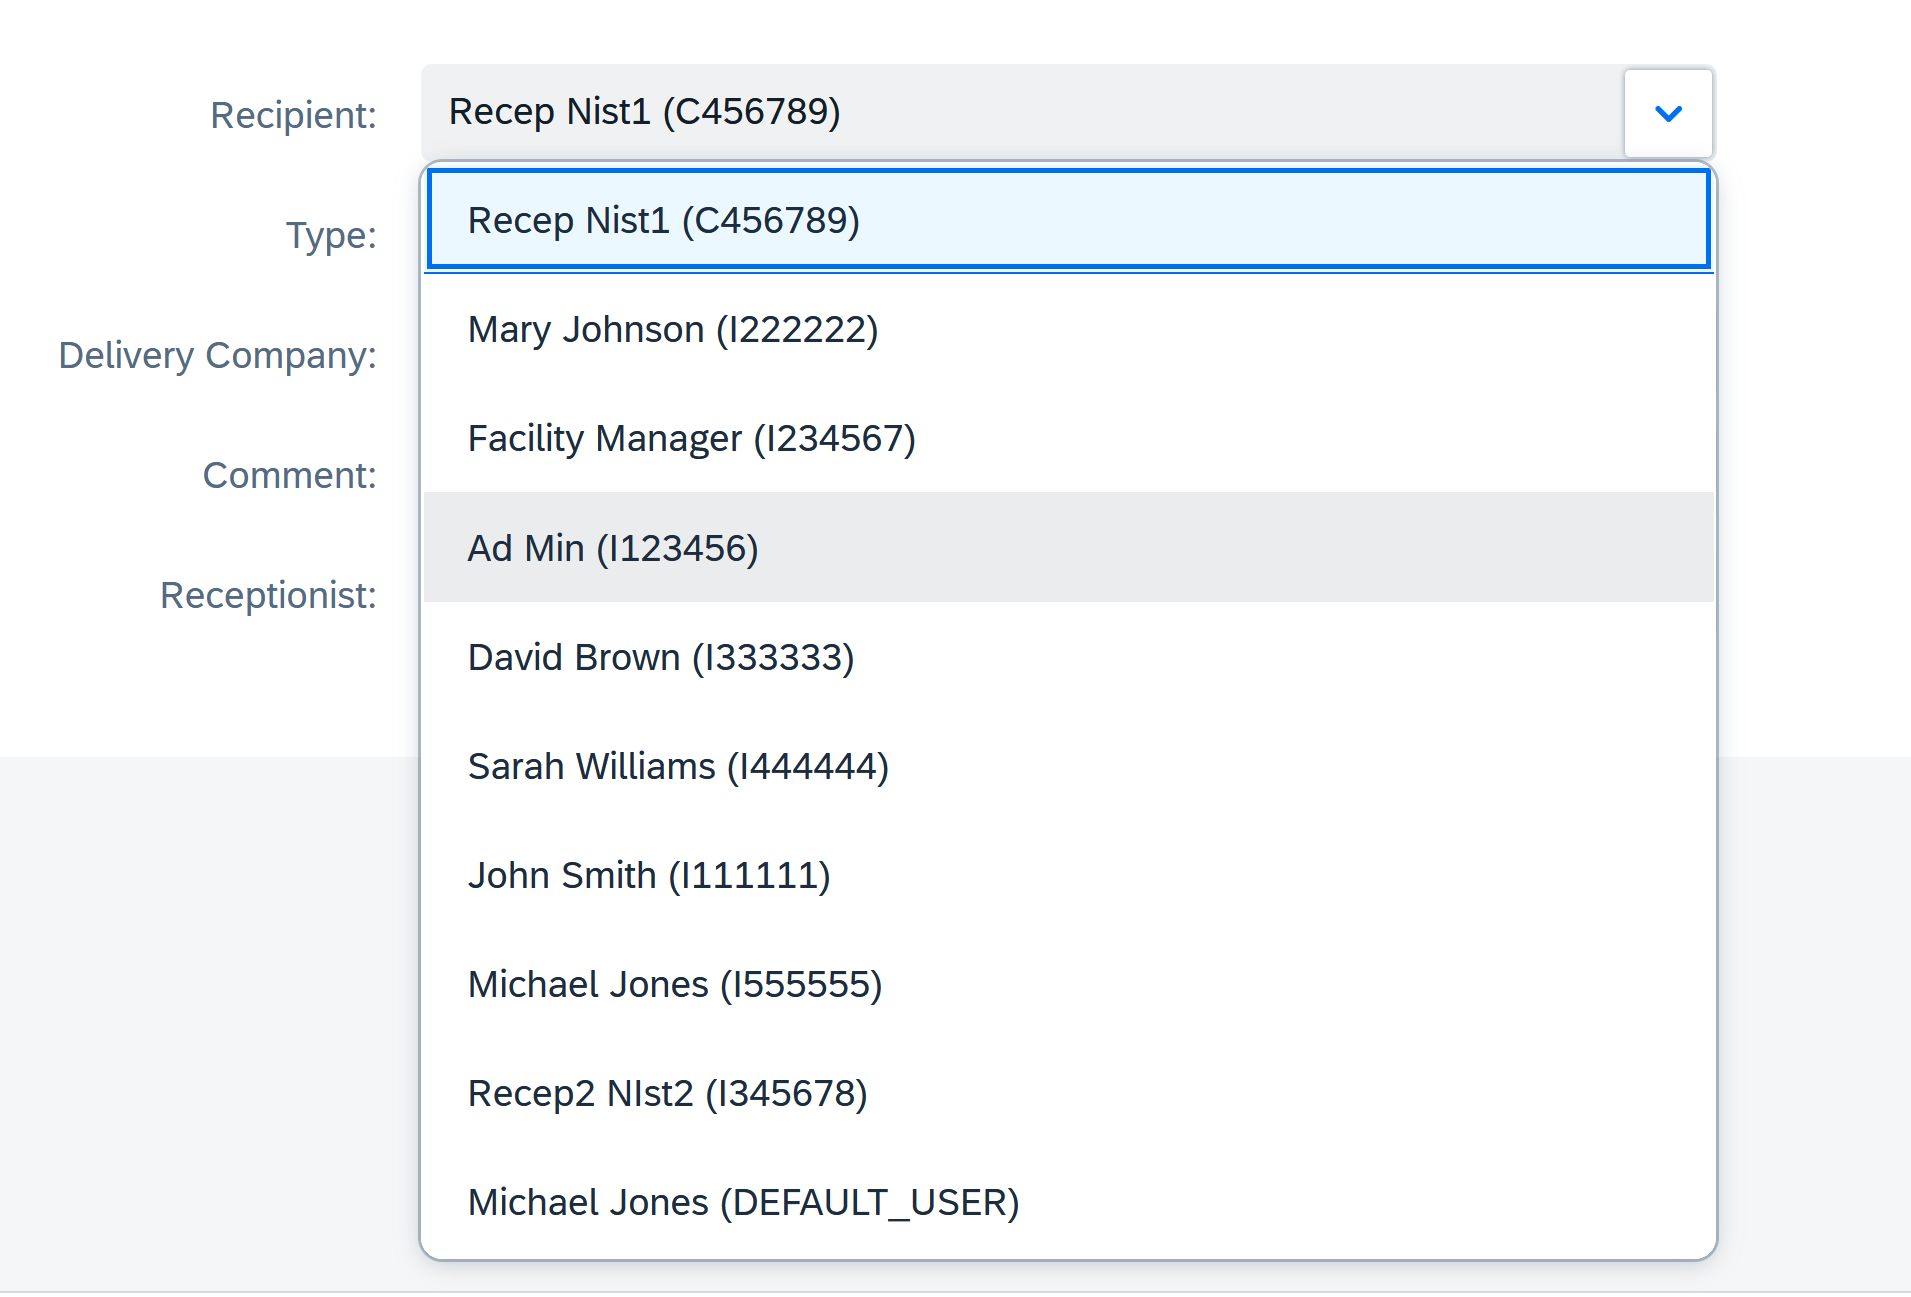
\includegraphics[width=0.45\linewidth]{images/user_doc/registration/entry1.png}}
   \hspace{5pt}
    \subcaptionbox{Step 2: Choose Package Type}{
		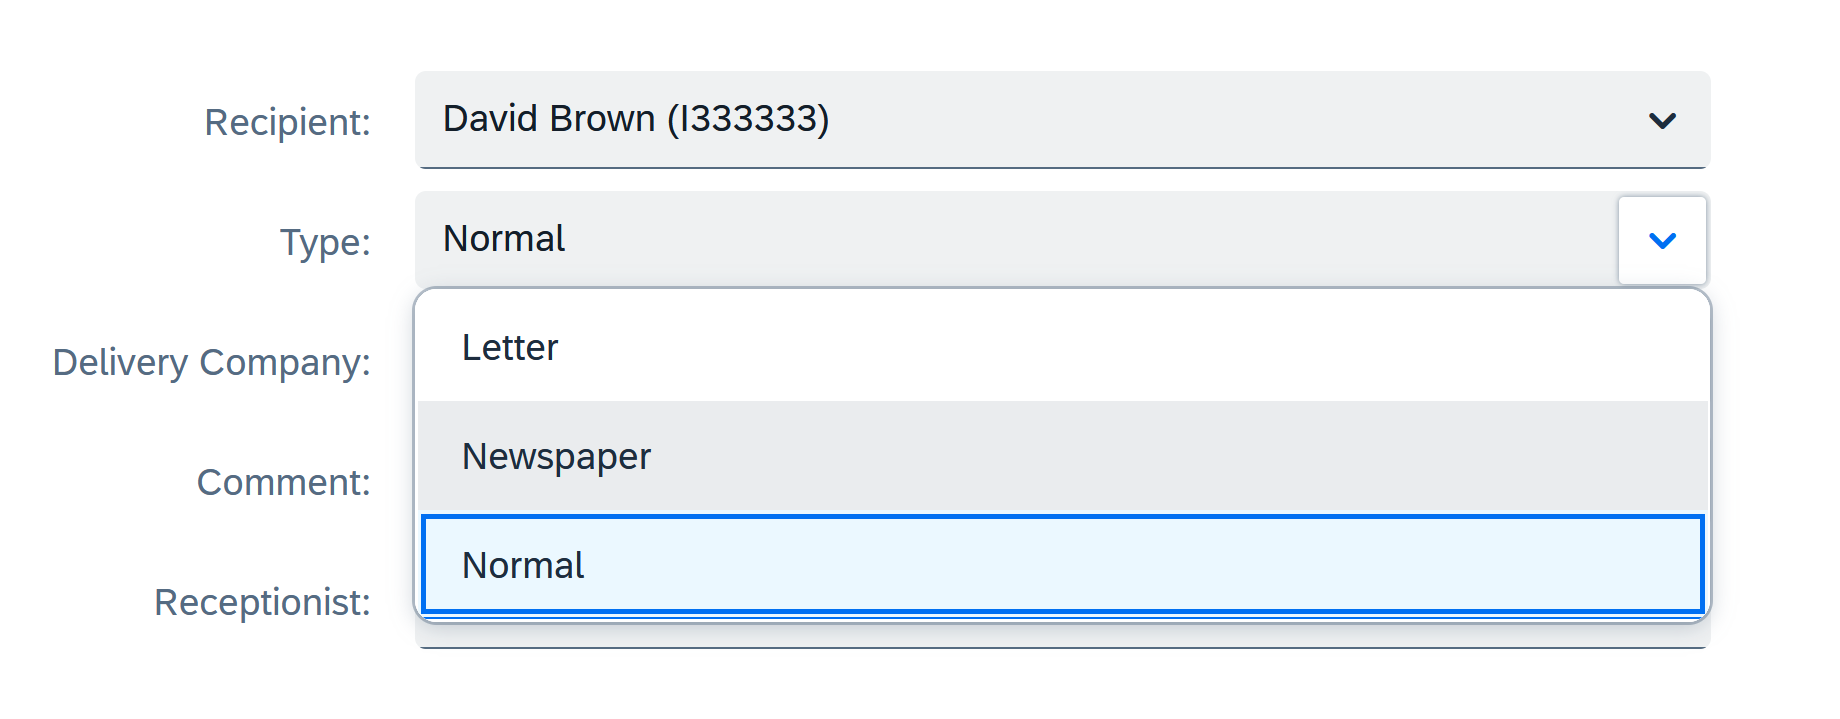
\includegraphics[width=0.45\linewidth]{images/user_doc/registration/entry2.png}}

    \vspace{10pt}
	\subcaptionbox{Step 3: Choose Delivery Company}{
		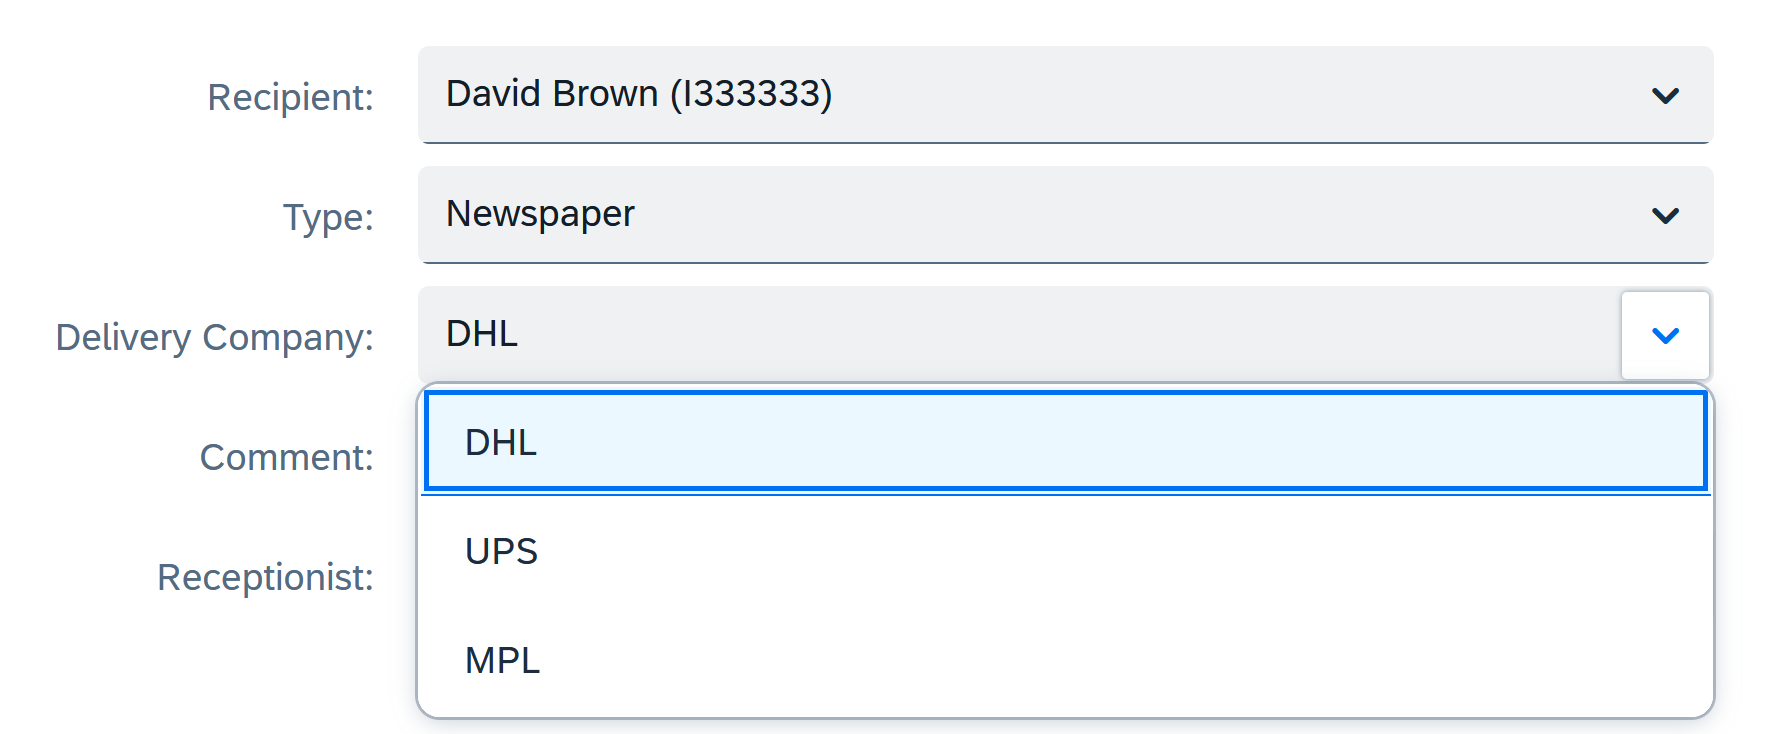
\includegraphics[width=0.45\linewidth]{images/user_doc/registration/entry3.png}}
    \hspace{5pt}
    \subcaptionbox{Step 4: Input any Comment if Needed}{
		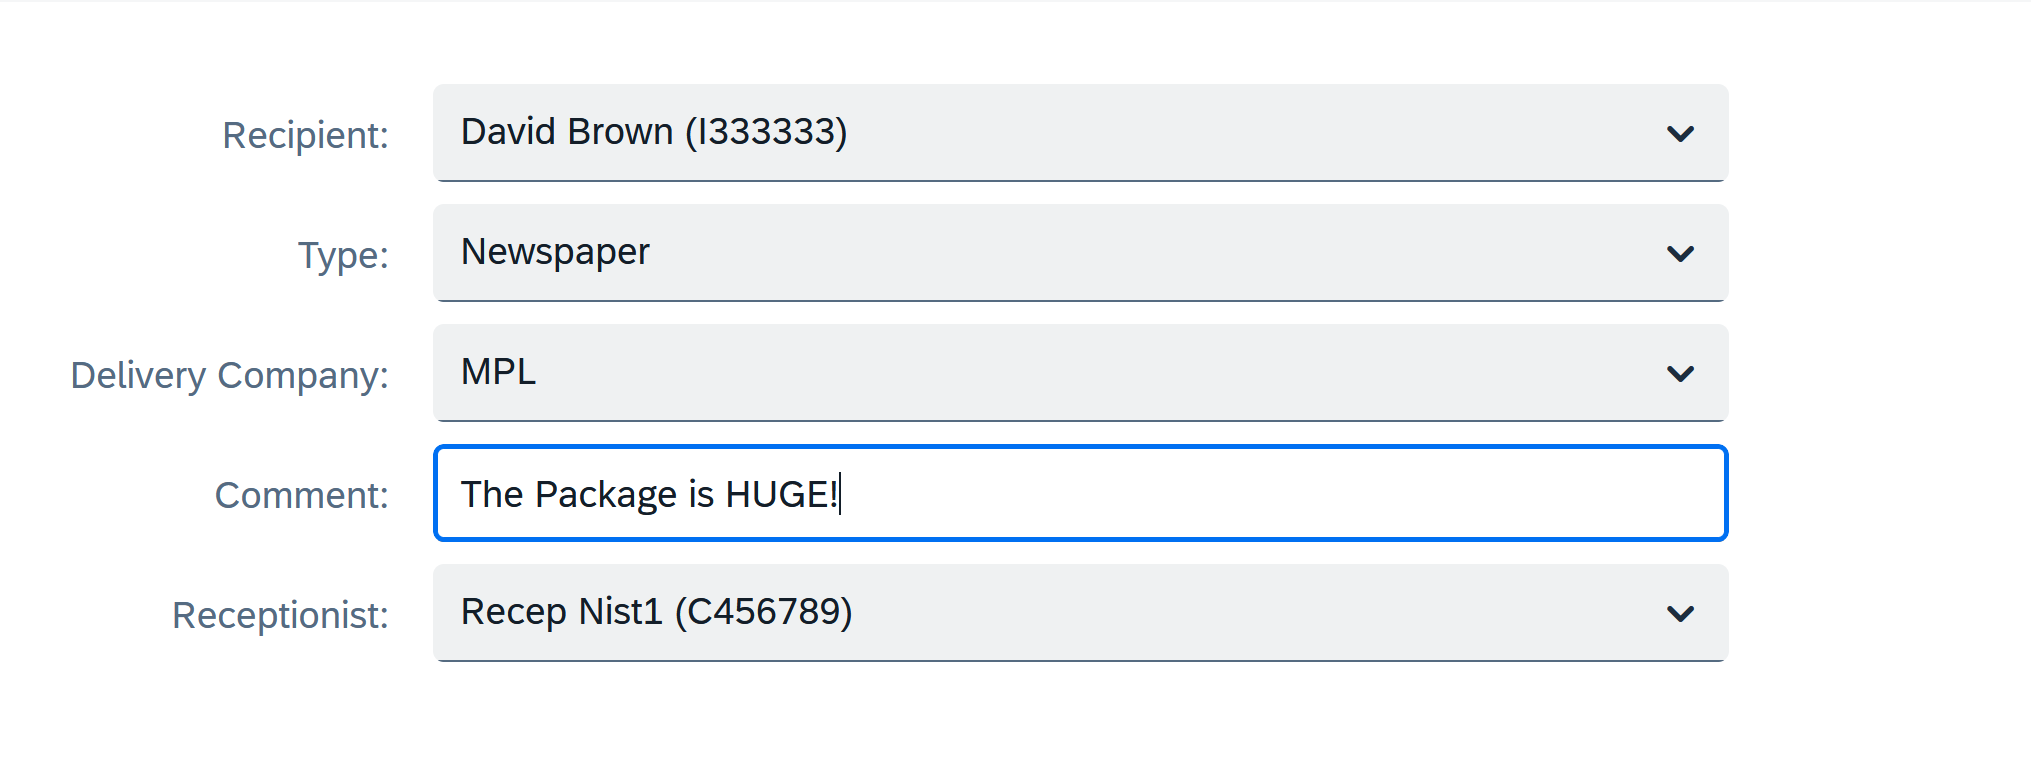
\includegraphics[width=0.45\linewidth]{images/user_doc/registration/entry4.png}}

    \vspace{10pt}
    	\subcaptionbox{Step 5: Choose Responsible Receptionist}{
		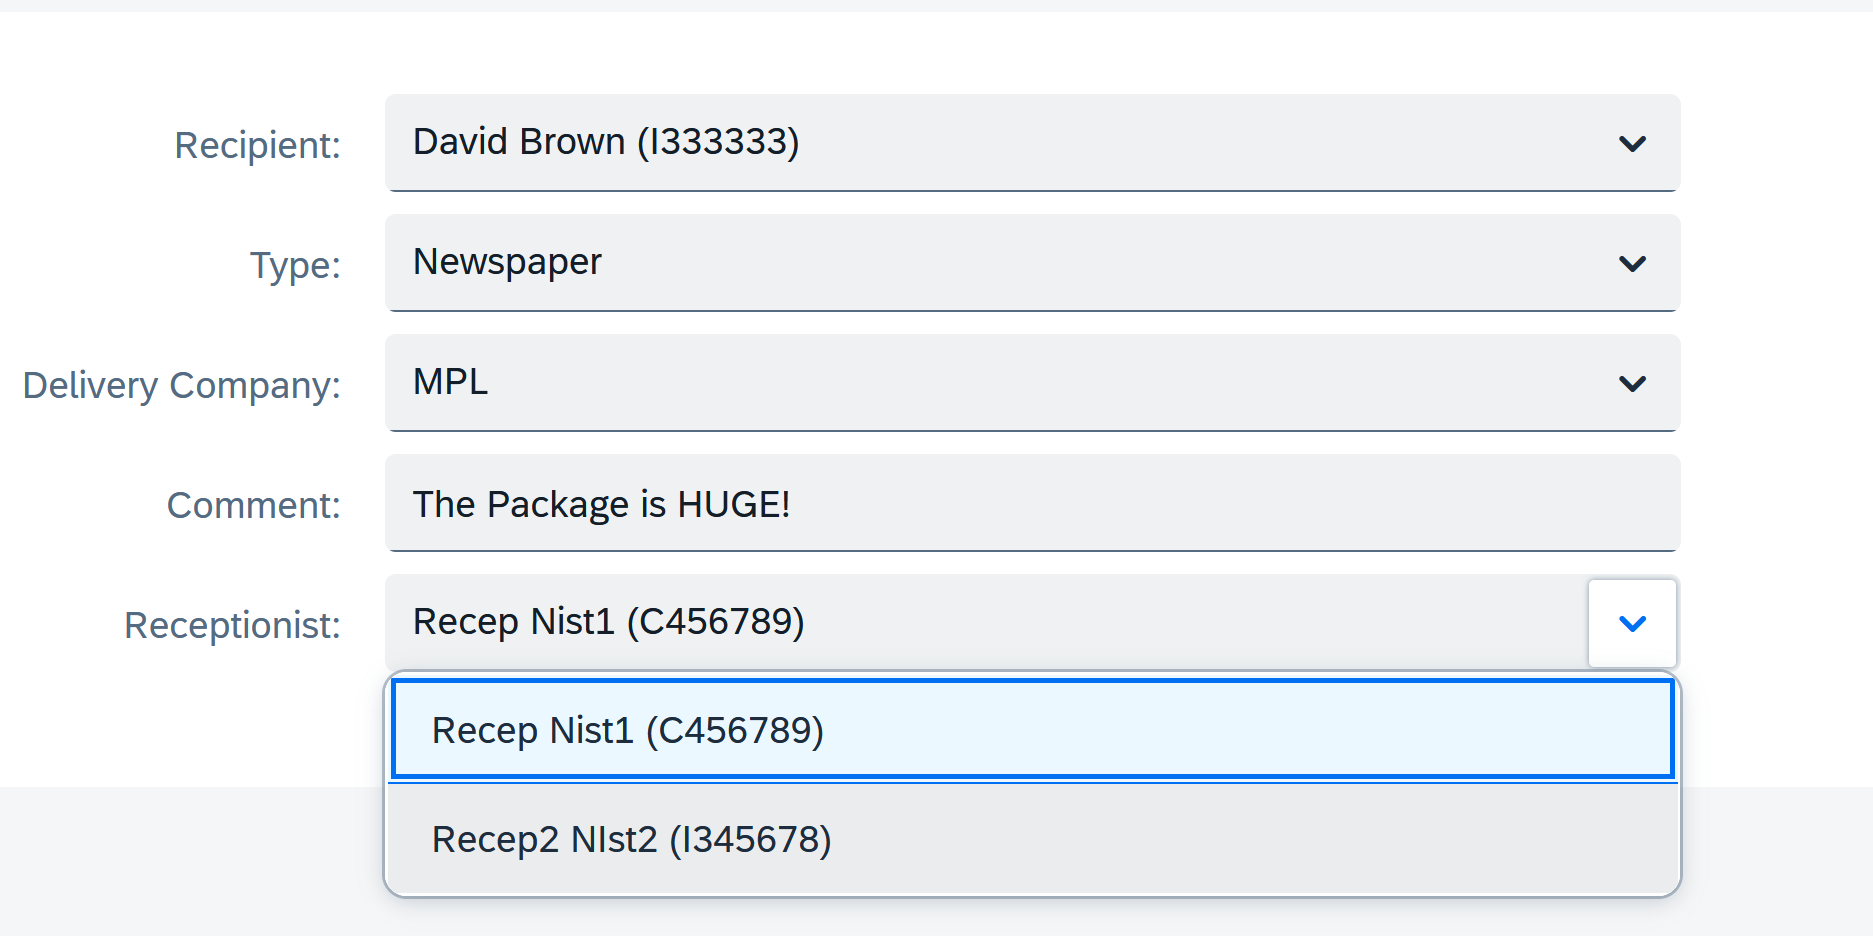
\includegraphics[width=0.45\linewidth]{images/user_doc/registration/entry5.png}}
  
    \caption{Package Registration Form - Form Entry Guide}
	\label{fig:RPformEntry}
\end{figure}

\subsubsection{Data Submitting}

If the "Save" button is clicked, the entered package details are submitted, a package with \textit{new} status is created in the system, a success message toast appears and the \textbf{Receptionist} is then navigated automatically to the \textbf{Manage Package} application (\autoref{fig:RPsaveOp}).

If the "Save and New" button is clicked, the entered package details are submitted, a package with \textit{new} status is created in the system, a success message toast appears and the form is reset to default state. The \textbf{Receptionist} may then start to register another package (\autoref{fig:RPsaveNewOp}).

If the "Discard" button is clicked, the form is reset to default state and \textbf{Receptionist} is navigated back to the launch pad (\autoref{fig:RPdiscardOp}). 

\begin{figure}[htb]
	\centering
    \begin{subfigure}{1\linewidth}
        \centering
        \subcaptionbox {Success Toast}{
            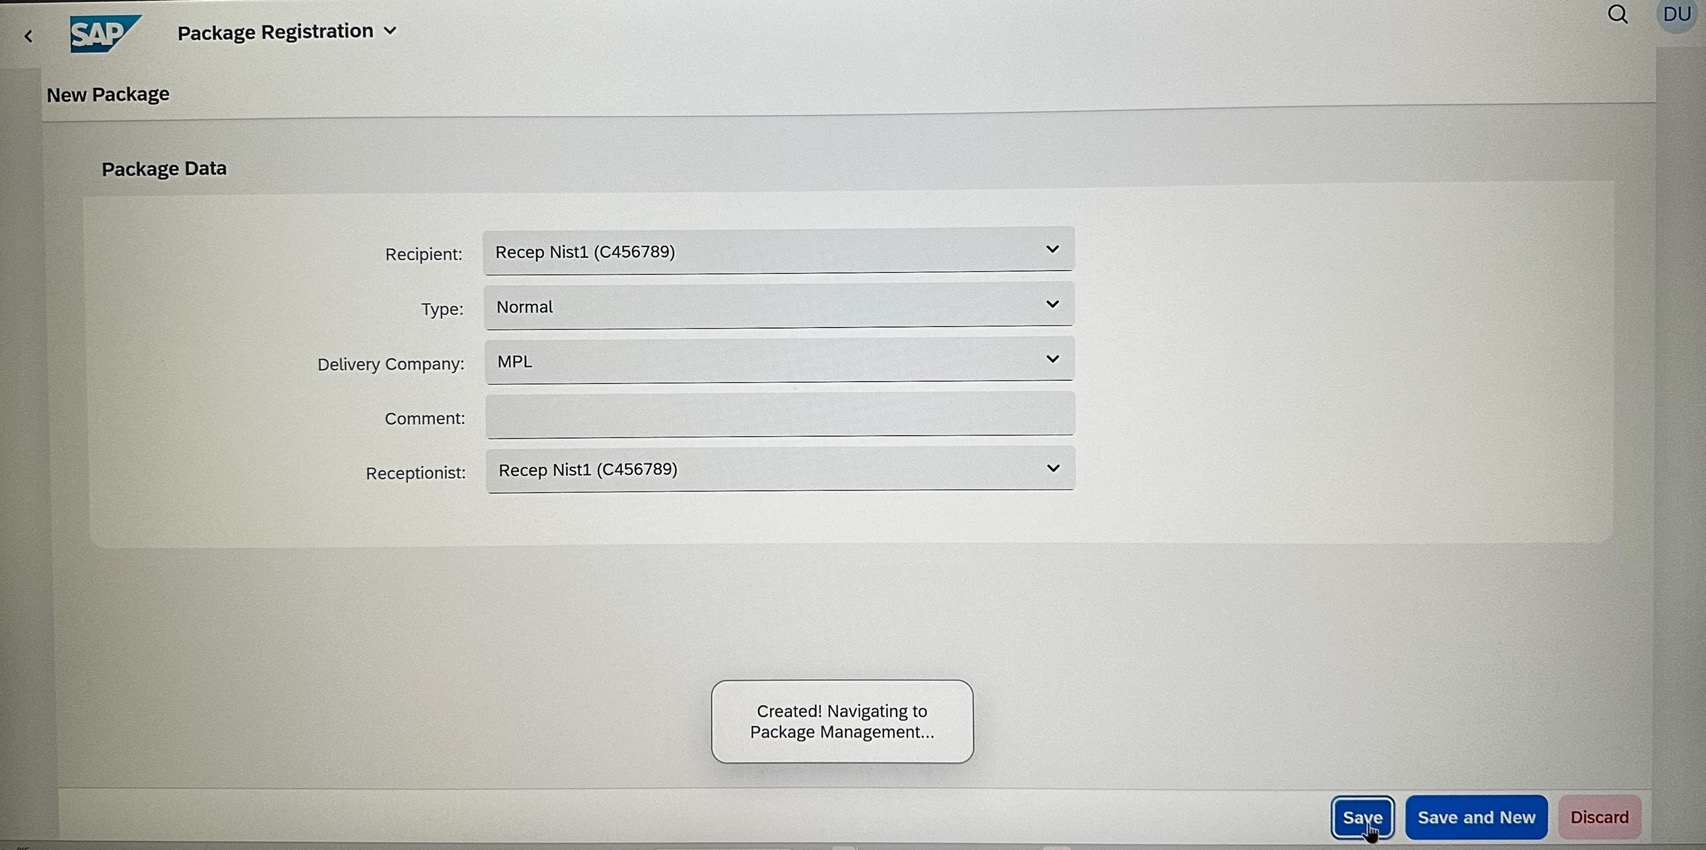
\includegraphics[width=0.5\linewidth]{images/user_doc/registration/SaveToast.jpg}
        }
        \vspace{5pt}
        \subcaptionbox {Target Navigation - Manage Package}{
            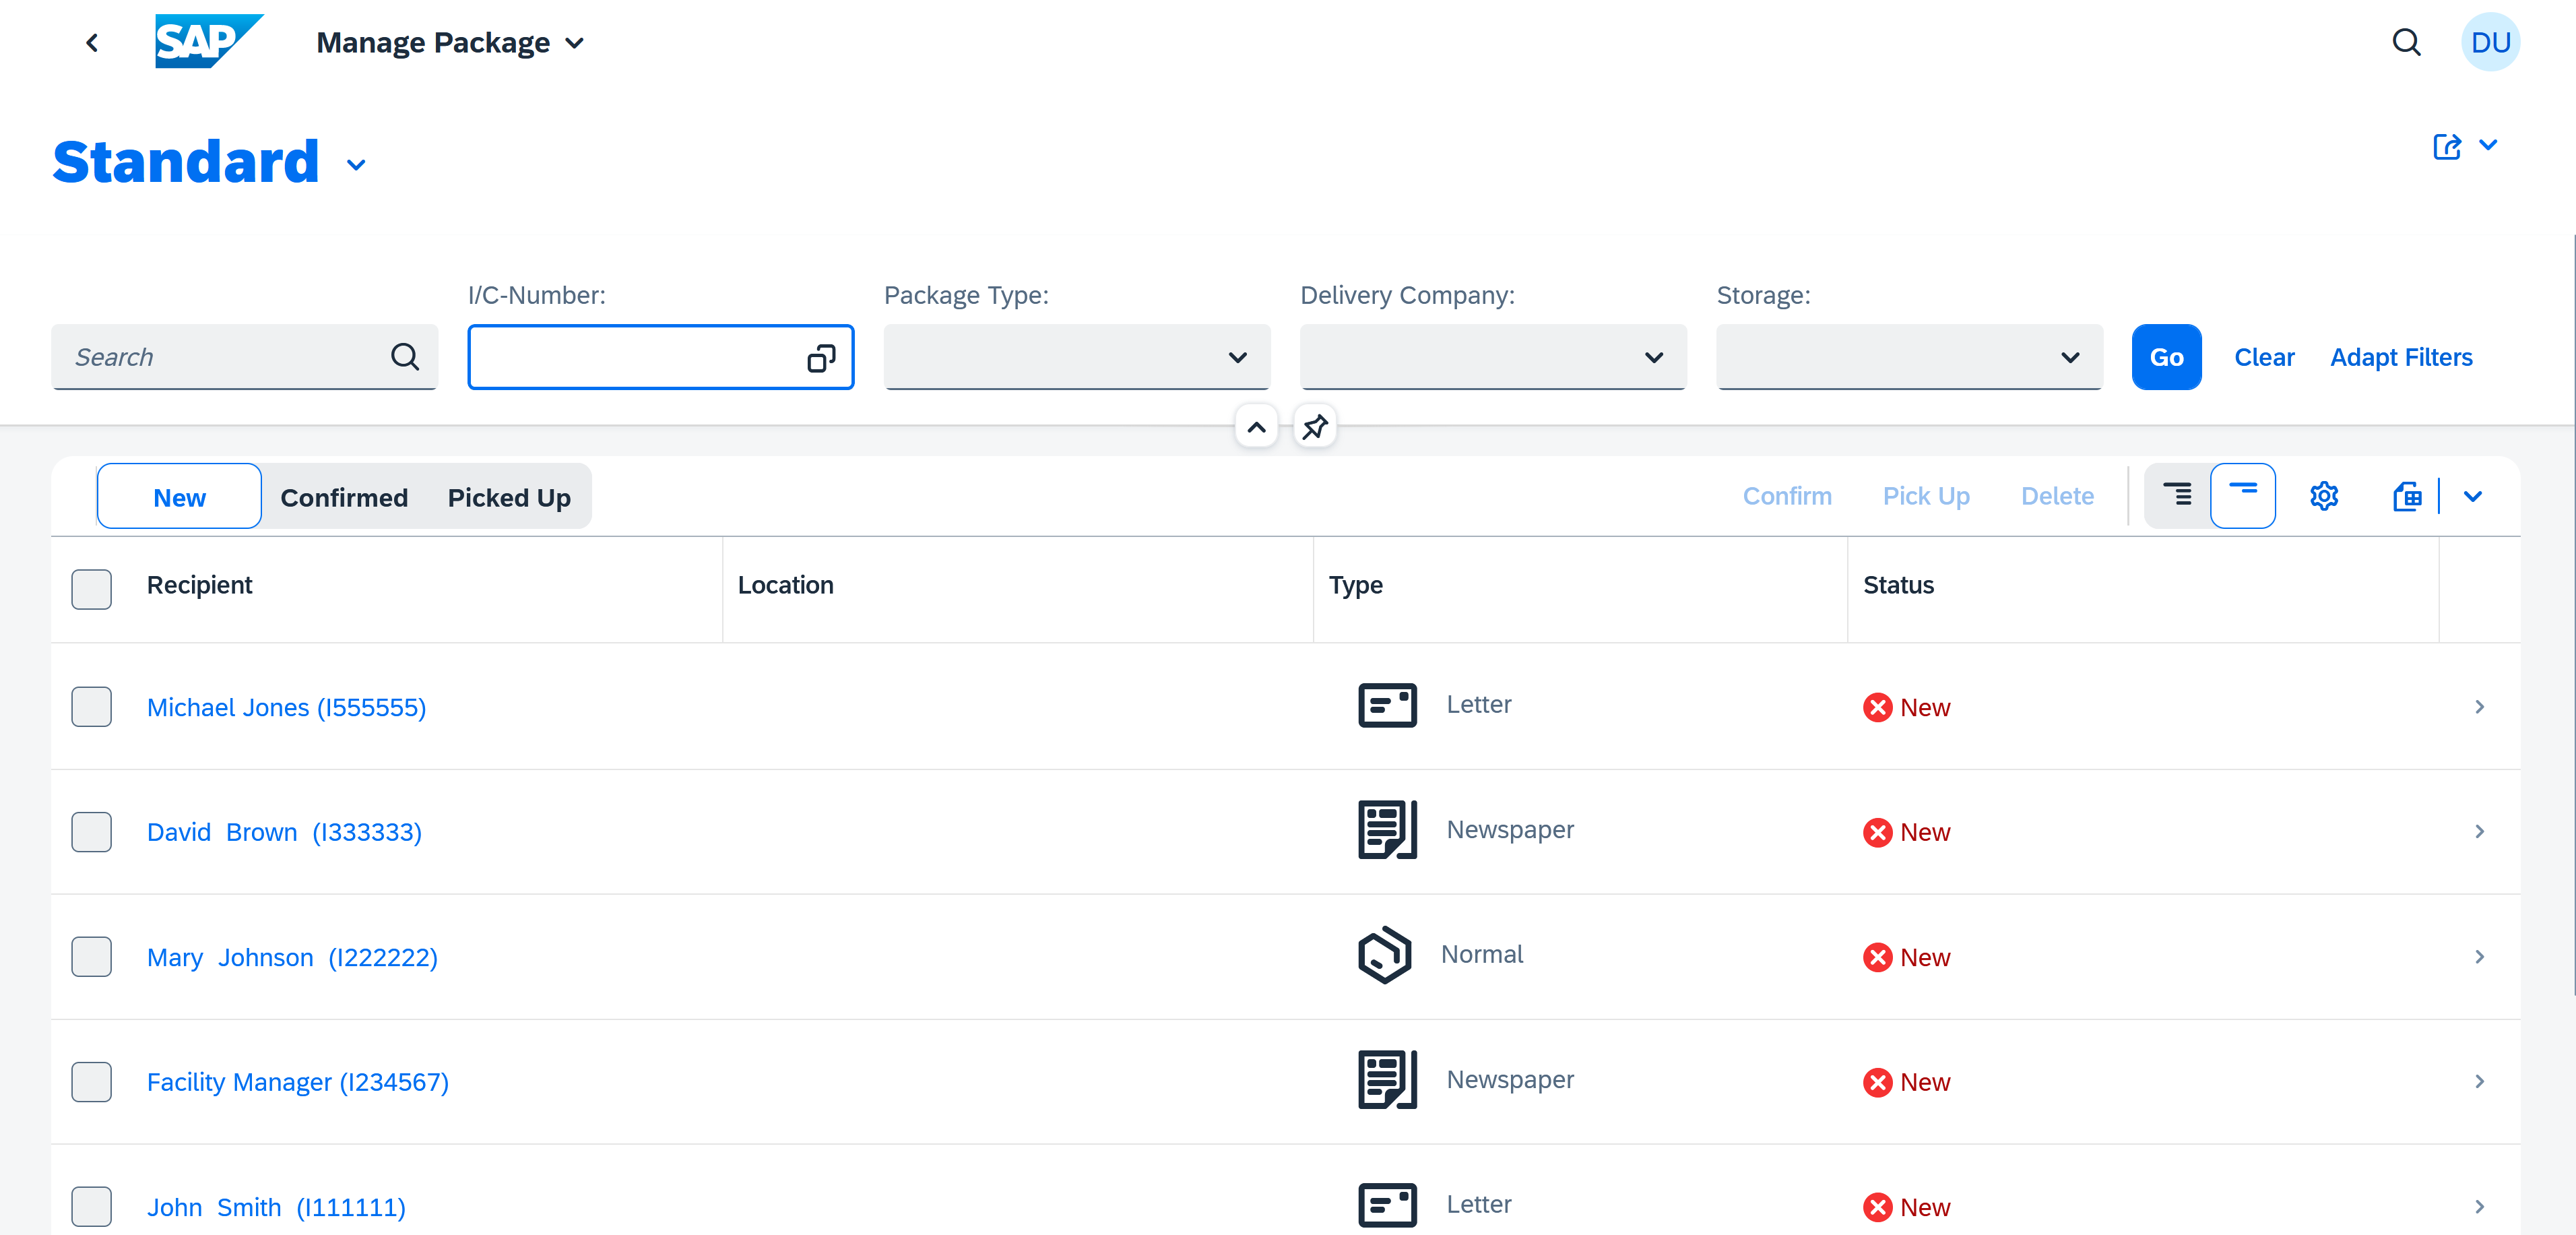
\includegraphics[width=0.5\linewidth]{images/user_doc/registration/target.png}
        }
    \end{subfigure}%
    \caption{Register Packages Form - Option 1: Save}
    \label{fig:RPsaveOp}
\end{figure}

\begin{figure}[htb!]
	\centering
    \begin{subfigure}{0.95\linewidth}
        \centering
        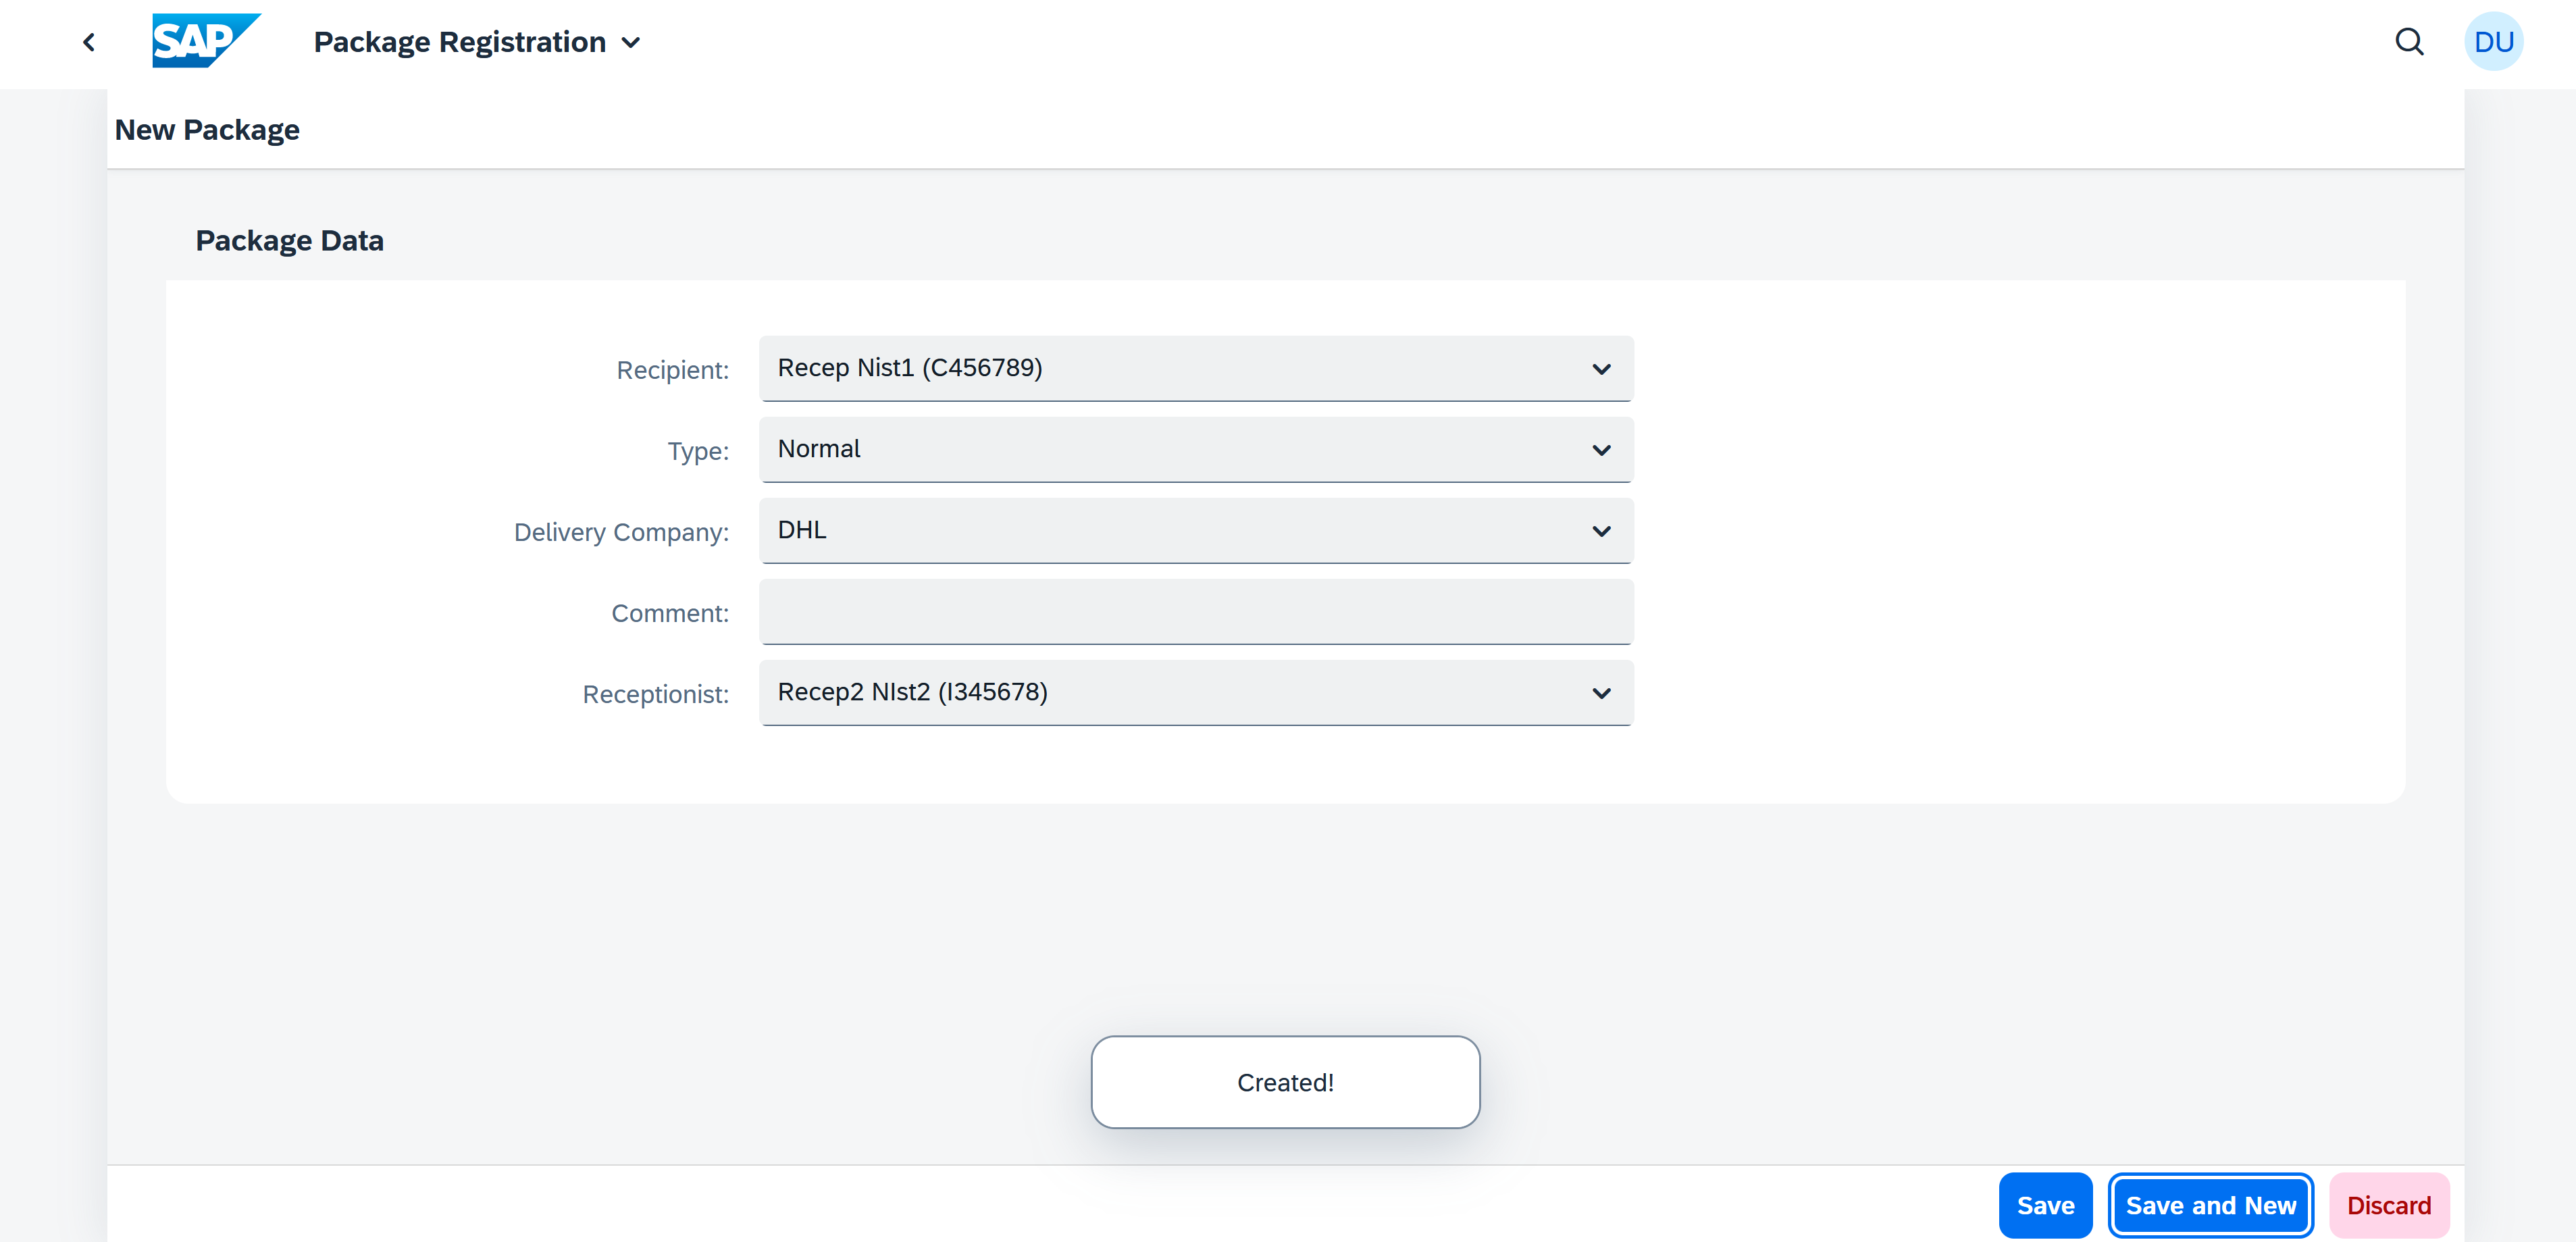
\includegraphics[width=1\linewidth]{images/user_doc/registration/saveAndNewToast.png}
    \end{subfigure}
    \caption{Register Packages Form - Option 2: Save and New}
    \label{fig:RPsaveNewOp}
\end{figure}

\begin{figure}[H]
	\centering
    \begin{subfigure}{0.95\linewidth}
        \centering
        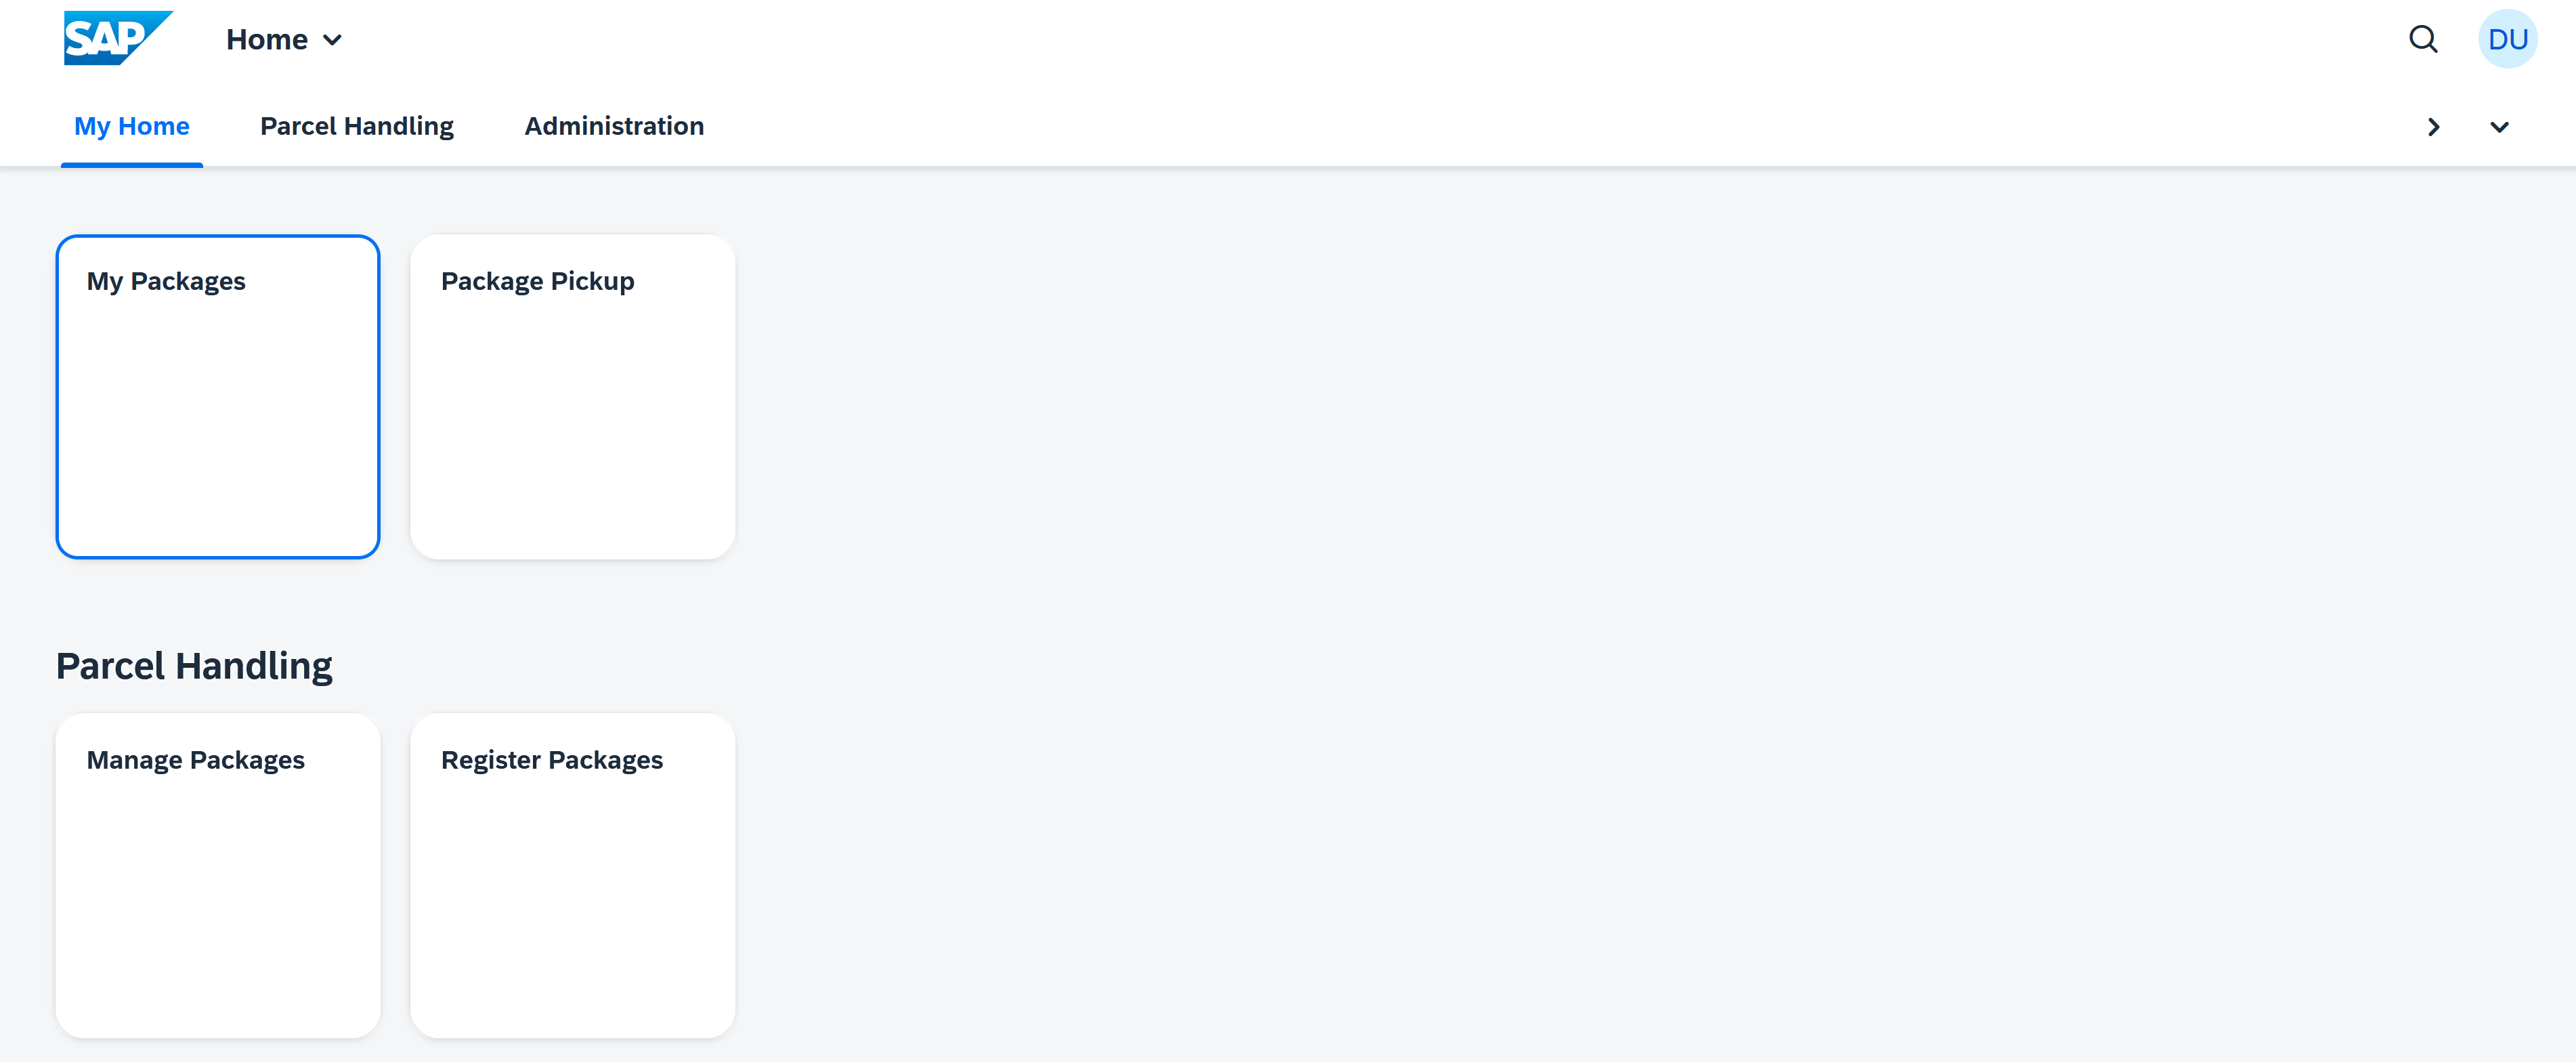
\includegraphics[width=1\linewidth]{images/user_doc/registration/discardTarget.png}
    \end{subfigure}
    \caption{Package Registration Form - Option 3: Discard}
    \label{fig:RPdiscardOp}
\end{figure}

\bigskip
\subsection{Manage Packages}                     
\label{subsec:mp}

The \textbf{Manage Packages} application is designed for the \textbf{Receptionist} (See \autoref{sec:UdocReceptionist} for all receptionist related applications) to edit, confirm, pickup, check the existing packages in the system. The reader can navigate to \autoref{subsec:dev-ui-mp} for more implementation details. The summarized main actions a \textbf{Receptionist} can take are listed here:

\begin{compactenum}
	\item Browse the existing packages.
        \begin{compactenum}
            \item Filtering possibility.
            \item Quick variant switch based on package status.
            \item Report List of packages info with selection capability.
            \item Detail page for single packages.
        \end{compactenum}
    \item Confirm package(s) with status \textit{new}.
    \item Pickup a package (single at a time) with status \textit{confirmed}. (As a backup maneuver in case the employee cannot access to mobile devices.
    \item Delete package(s) with status \textit{new} or \textit{confirmed}.
    \item Edit package(s)' recipient, type, delivery company, and comment.
\end{compactenum}

\bigskip
\begin{figure}[H]
	\centering
	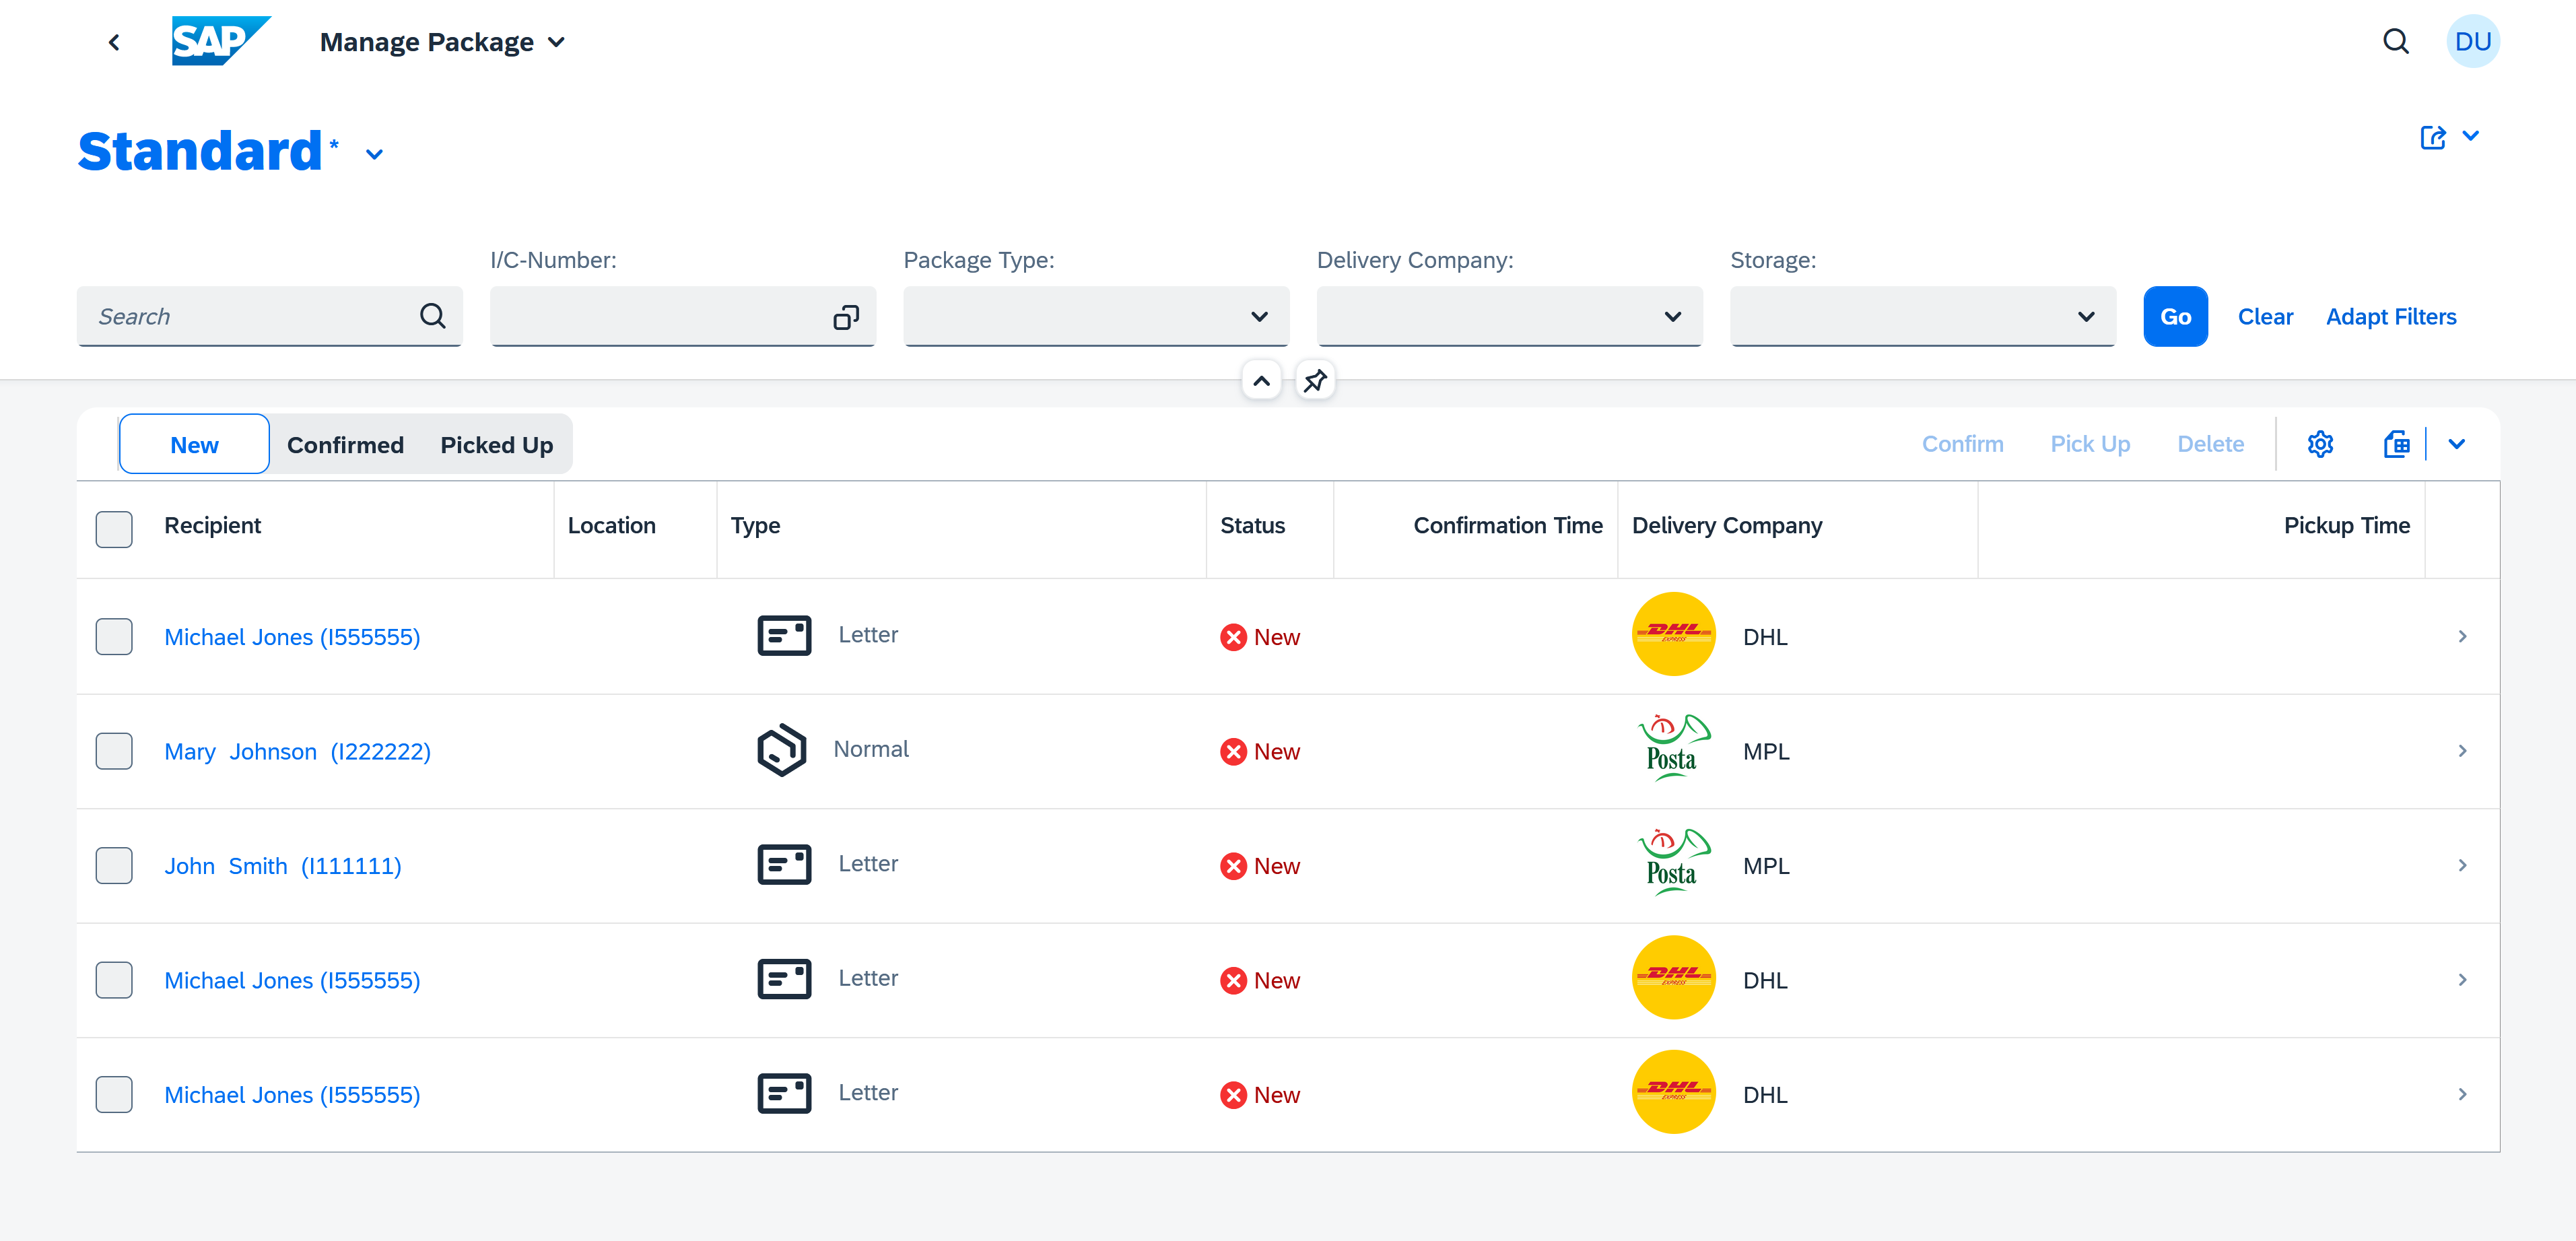
\includegraphics[height=200pt]{images/user_doc/managePack/ReportScreen/browse/Overview.png}
	\caption{Manage Packages Report Screen - Overview}
	\label{fig:MPReportOverview}
\end{figure}


\subsubsection{Browse Packages}
After clicking at the application tile, the \textbf{Receptionist} is redirected to the "Report Screen"(\autoref{fig:MPReportOverview}). 
The upper part displays the search bar and the possible filters (\autoref{fig:MPFIlterBar}). 

\begin{figure}[H]
	\centering
	
\includegraphics[width=1\linewidth]{images/user_doc/managePack/ReportScreen/browse/FilterBar.png}
	\caption{Manage Packages Report Screen - Filter Bar}
	\label{fig:MPFIlterBar}
\end{figure}

In case the need of free text search of any possible content of the column, the \textbf{"Search Bar"} can be used (\autoref{fig:MPSearchBar}). The search supports in-completed keywords and is case insensitive. 

Predefined filters can also be used, where value helps and entry helps are provided.
The default predefined filters are: \textbf{I/C-Number} (free text SAP ID input, \autoref{fig:MPIDFIlter}), \textbf{Type} (drop down menu of all available types), \textbf{Delivery Company} (drop down menu of all available companies) and \textbf{Storage} (drop down menu of all available storages). 
For any drop down filters, zero to many options can be selected from the menu (\autoref{fig:MPDefaultDropDown}). 

\bigskip

\begin{figure}[htb]
	\centering
	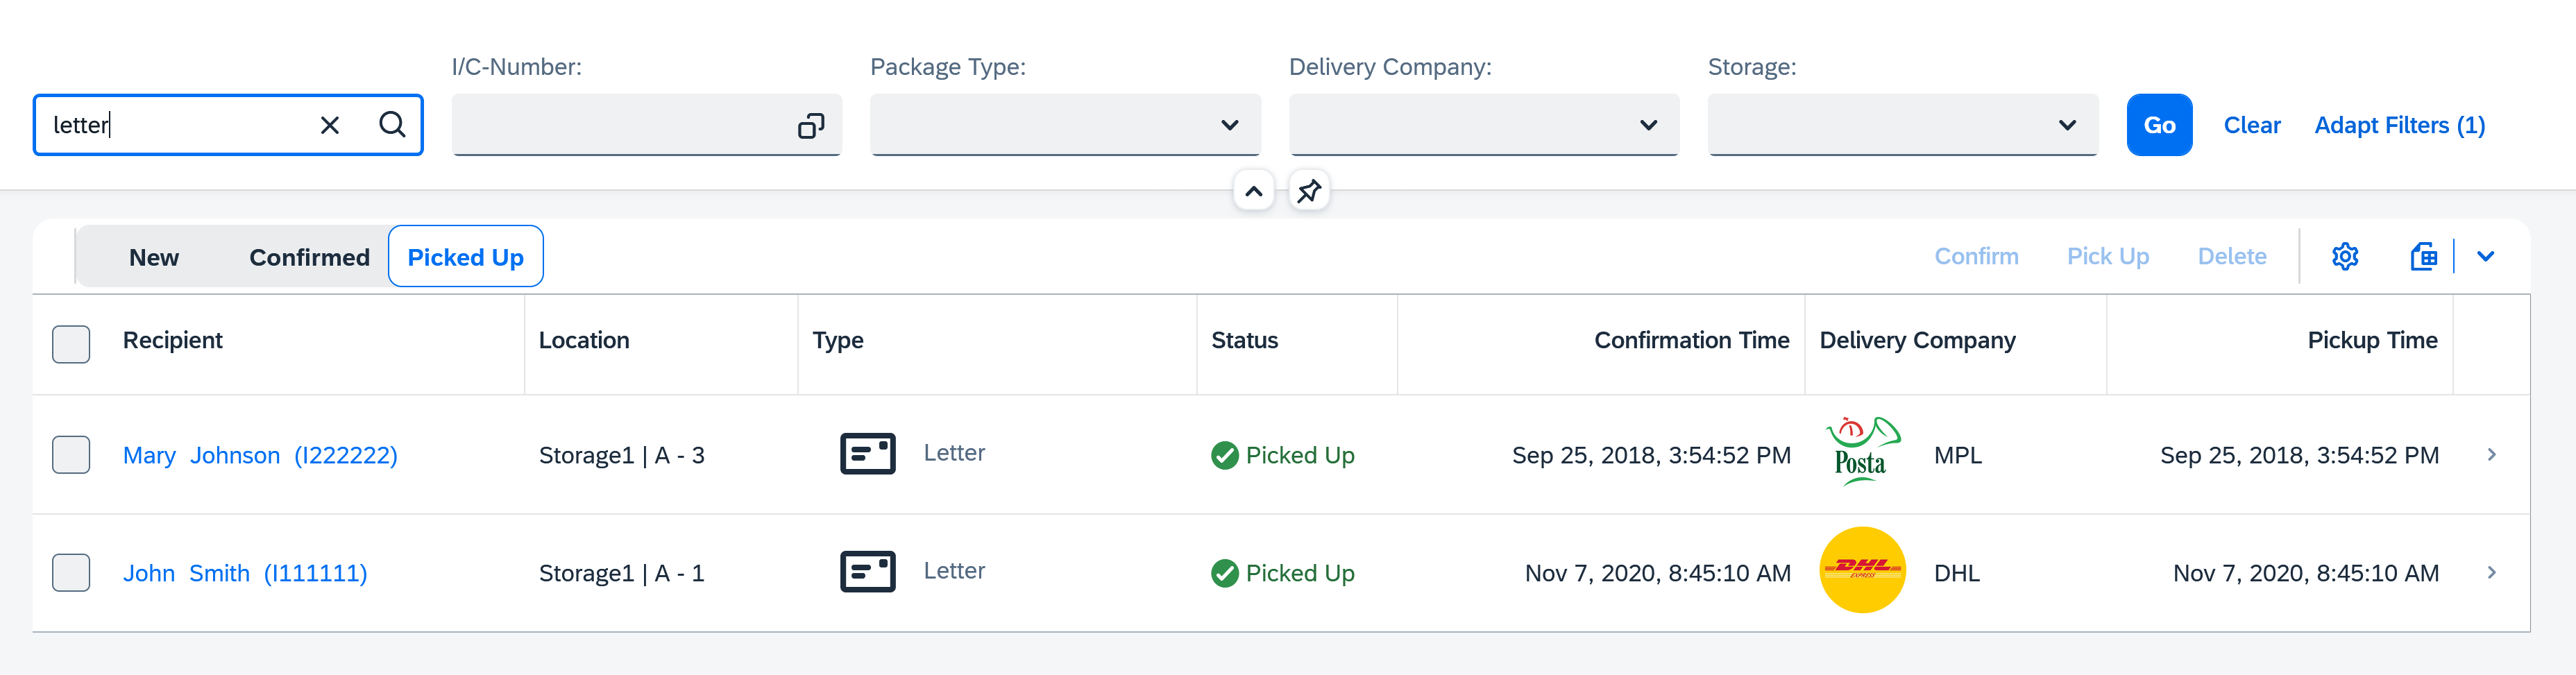
\includegraphics[width=1\linewidth]{images/user_doc/managePack/ReportScreen/browse/defaultSearchBarUsage.png}
	\caption{Manage Packages Report Screen - Filter Bar - Search Bar Usage Guide}
	\label{fig:MPSearchBar}
\end{figure}

\begin{figure}[htb]
	\centering
	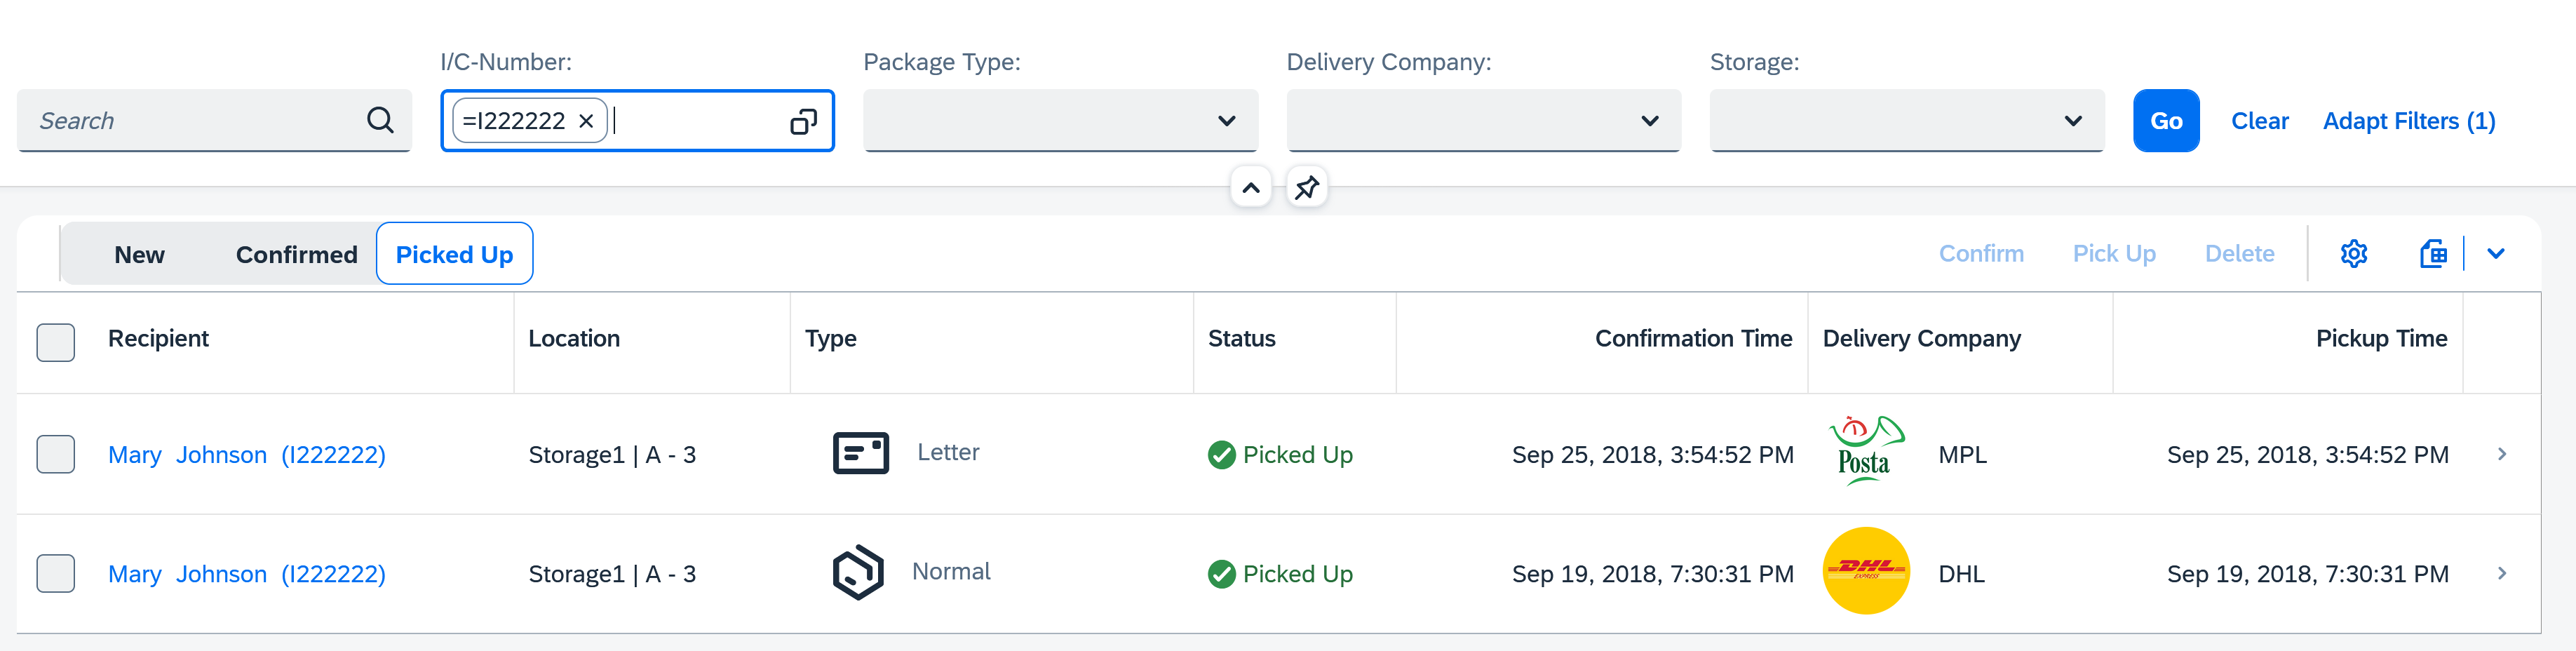
\includegraphics[width=1\linewidth]{images/user_doc/managePack/ReportScreen/browse/defaultFreeTextIdUsage.png}
	\caption{Manage Packages Report Screen - Filter Bar - ID Filter Usage Guide}
	\label{fig:MPIDFIlter}
\end{figure}


While adjusting the filtering values, the list view is temporarily locked. By clicking the "Go" Button, the adjusted filters are run and results will be displayed (\autoref{fig:MPAjustFilters}).


\begin{figure}[H]
	\centering
	\subcaptionbox{Type Filter}{
		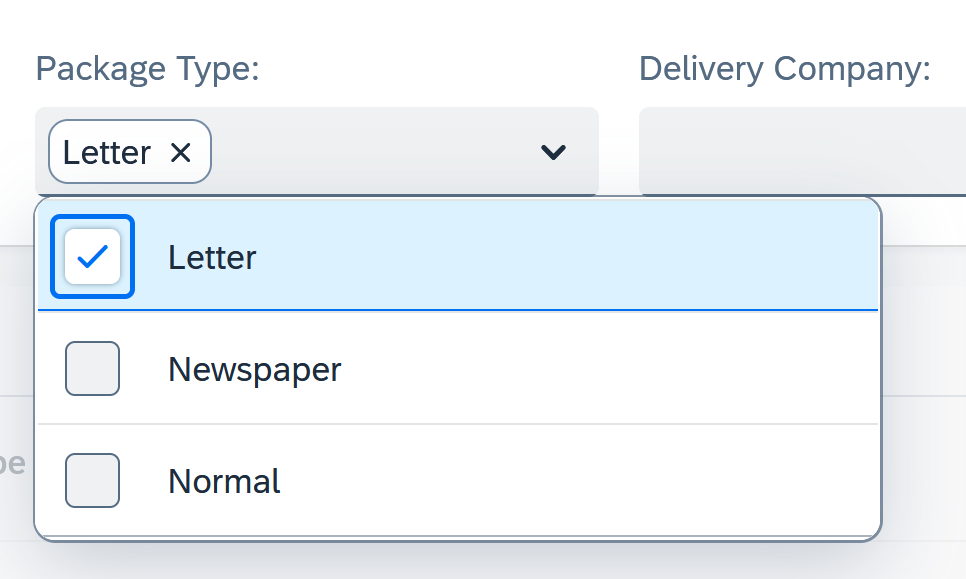
\includegraphics[width=0.45\linewidth]{images/user_doc/managePack/ReportScreen/browse/defaultType.png}}
	\hspace{5pt}
	\subcaptionbox{Company Filter}{
		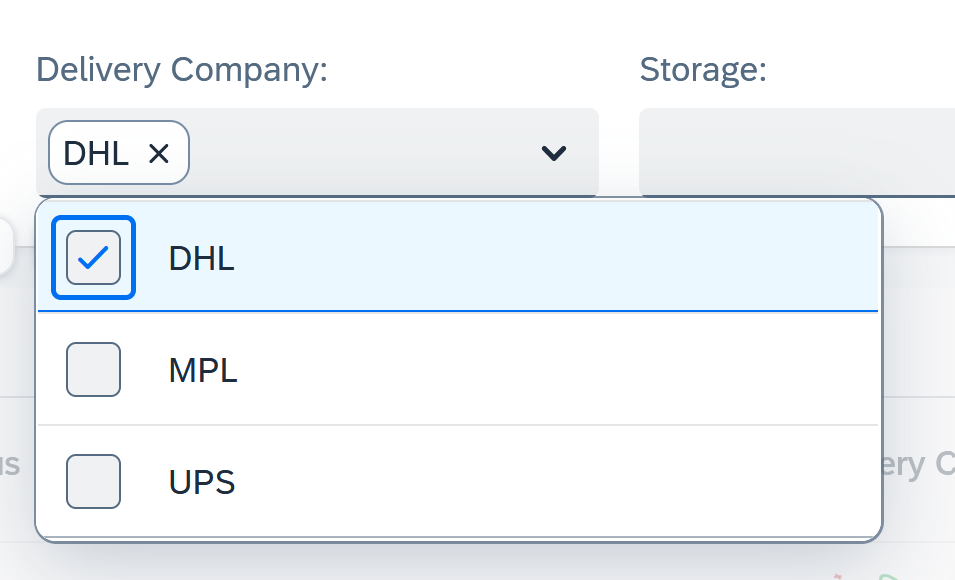
\includegraphics[width=0.45\linewidth]{images/user_doc/managePack/ReportScreen/browse/defaultCompany.png}}

    \subcaptionbox{Storage Filter}{
		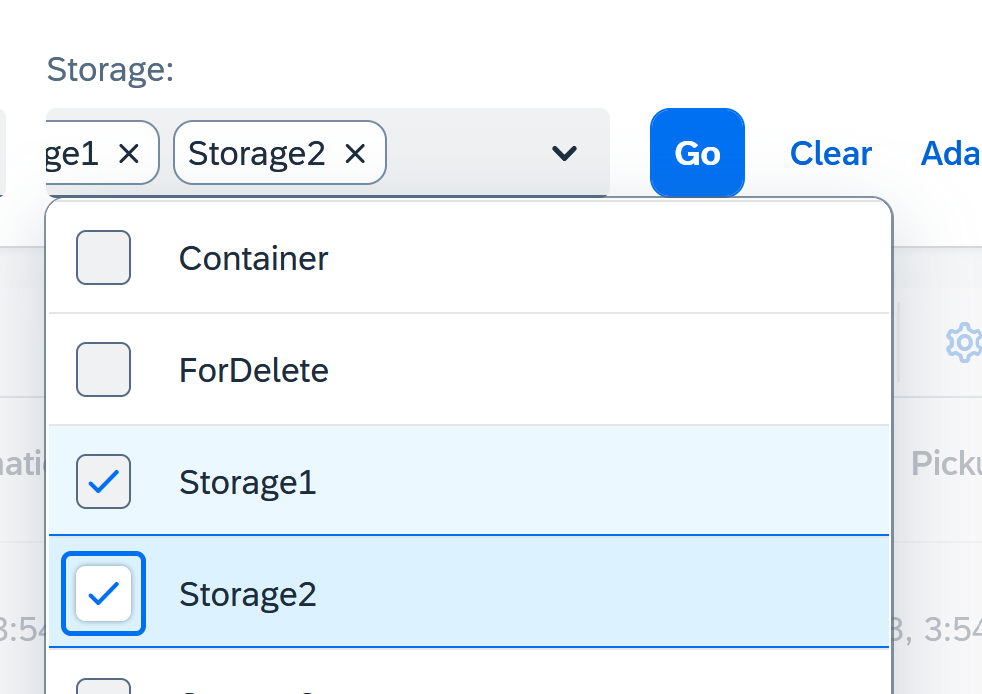
\includegraphics[width=0.45\linewidth]{images/user_doc/managePack/ReportScreen/browse/defaultStorage.png}}
	\caption{Manage Packages Report Screen - Filter Bar - Default Drop Down Filters Show Case}
	\label{fig:MPDefaultDropDown}
\end{figure}

\begin{figure}[htb]
		\centering
	\subcaptionbox{While Adjusting the Filter}{
		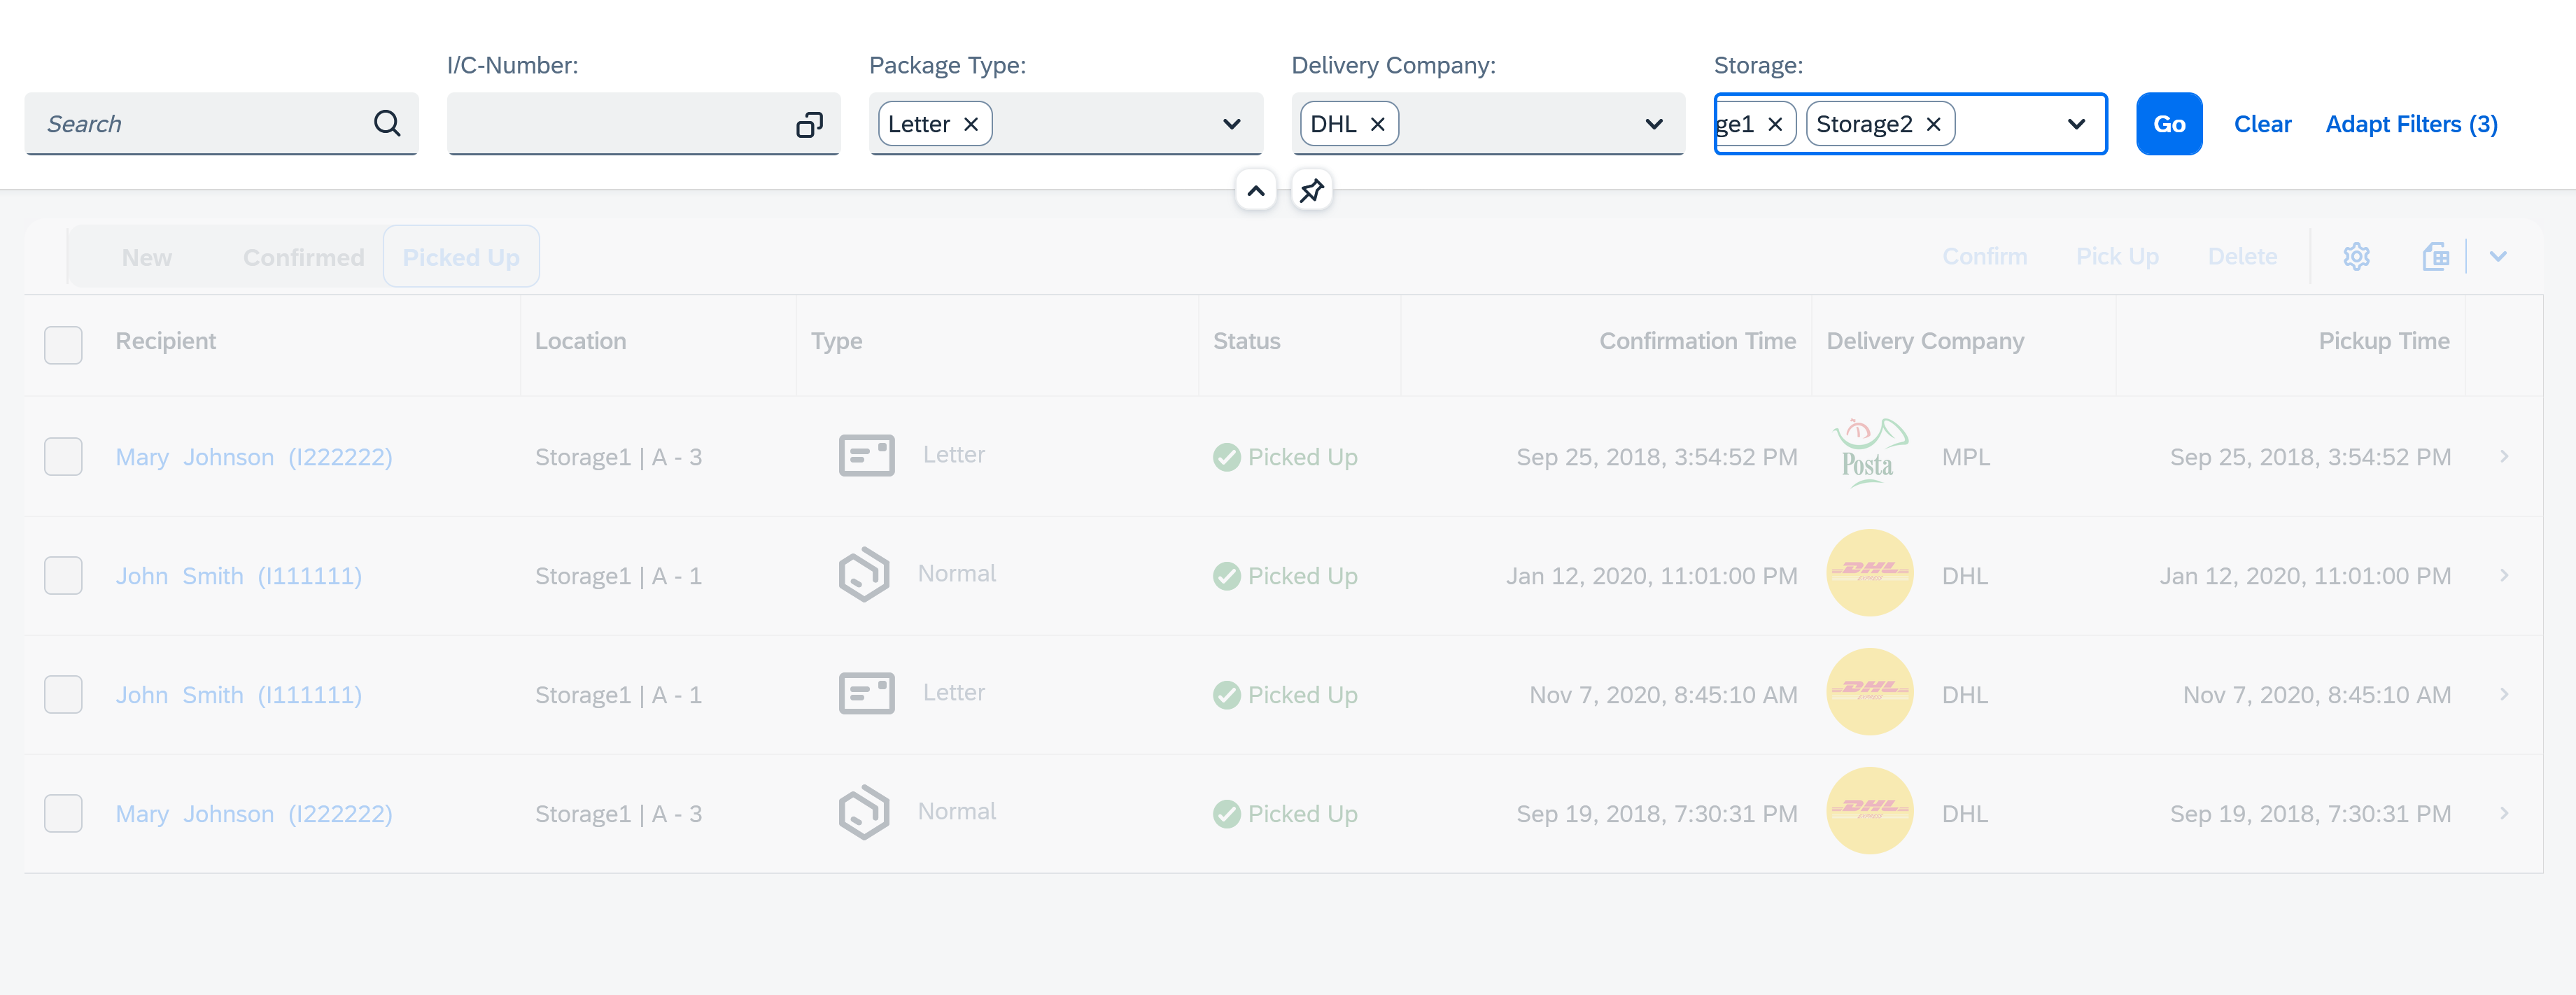
\includegraphics[width=0.9\linewidth]{images/user_doc/managePack/ReportScreen/browse/filterOnAdjusting.png}}
	\vspace{5pt}
 
	\subcaptionbox{Clicked "Go"}{
		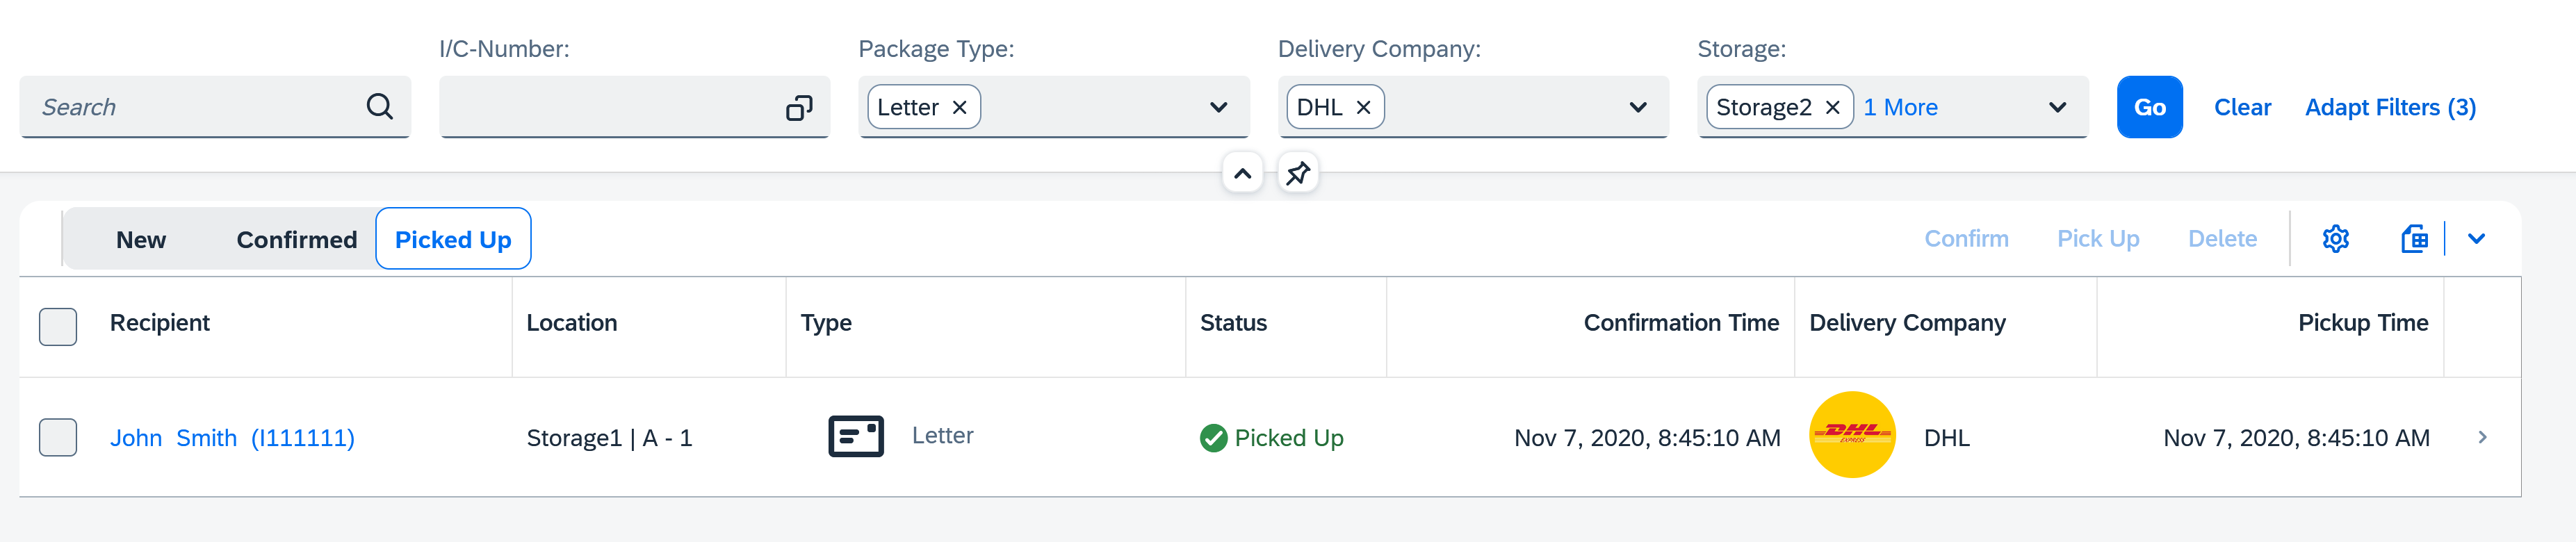
\includegraphics[width=0.9\linewidth]{images/user_doc/managePack/ReportScreen/browse/filterAfterGo.png}}
    \caption{Manage Package Report Screen - Adjust Filters}
    \label{fig:MPAjustFilters}
\end{figure}

In the middle there is a variant breadcrumb on the left and three action buttons on the right (\autoref{fig:MPMiddle}). The variant breadcrumb shows the three possible status of the packages. By selecting one of the variants, the list of packages with corresponding status are displayed (\autoref{fig:MPBreadCrumb}). The three action buttons are by default deactivated. They will be activated when certain conditions are full filled (i.e. the action can be performed).

\begin{figure}[H]
	\centering
	\subcaptionbox{Variants Bread}{
		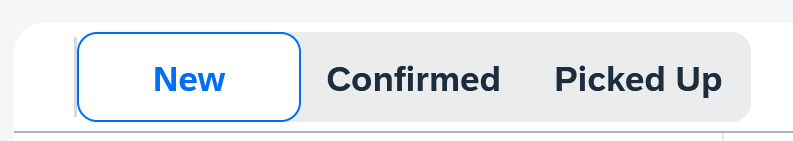
\includegraphics[width=0.45\linewidth]{images/user_doc/managePack/ReportScreen/browse/VariantsBread.png}}
	\hspace{5pt}
	\subcaptionbox{Action Buttons}{
		
\includegraphics[width=0.45\linewidth]{images/user_doc/managePack/ReportScreen/browse/buttonInactive.png}}
  \caption{Manage Packages Report Screen - Middle Control}
	\label{fig:MPMiddle}
\end{figure}


\begin{figure}[H]
	\centering
	\subcaptionbox{New Variant}{
		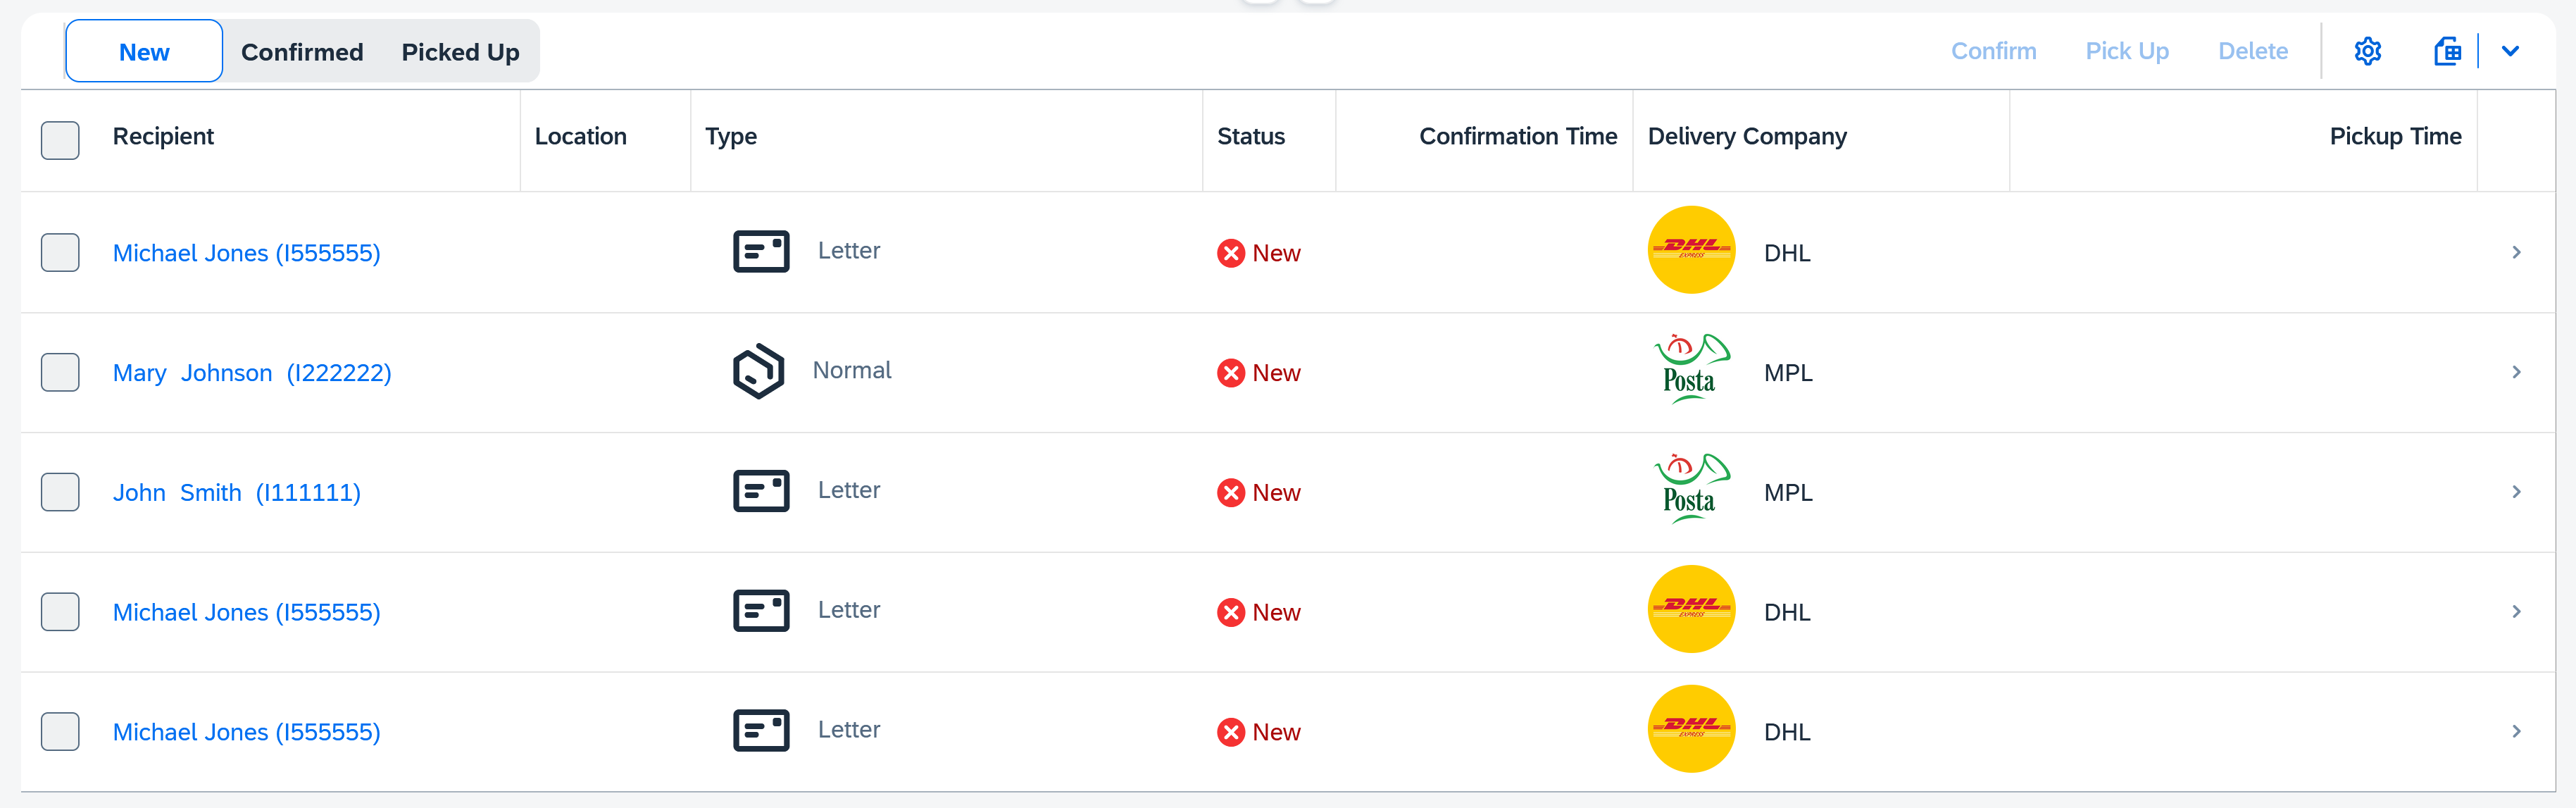
\includegraphics[width=0.85\linewidth]{images/user_doc/managePack/ReportScreen/browse/NewVariant.png}}
	\vspace{10pt}
 
	\subcaptionbox{Confirmed Variant}{
		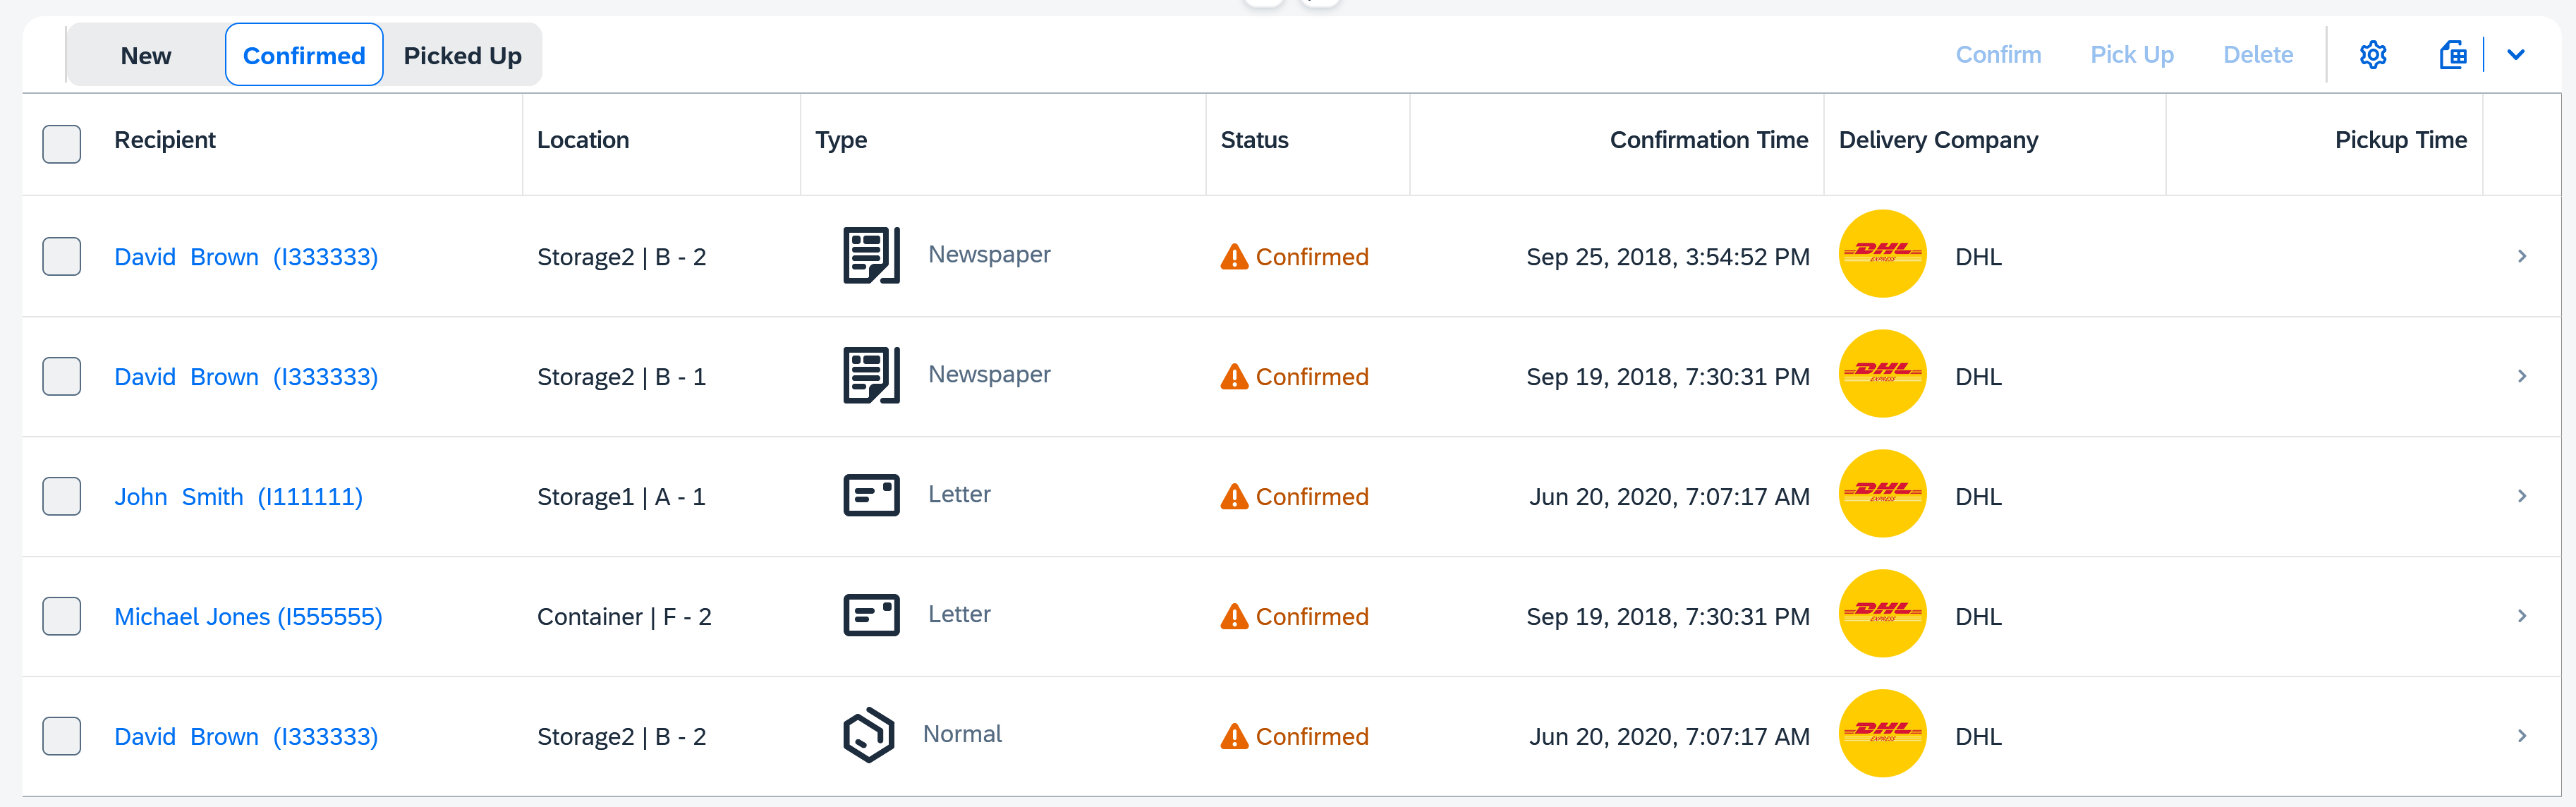
\includegraphics[width=0.85\linewidth]{images/user_doc/managePack/ReportScreen/browse/ConfirmedVariant.png}}

    \vspace{10pt}
    \subcaptionbox{Picked Up Variant}{
		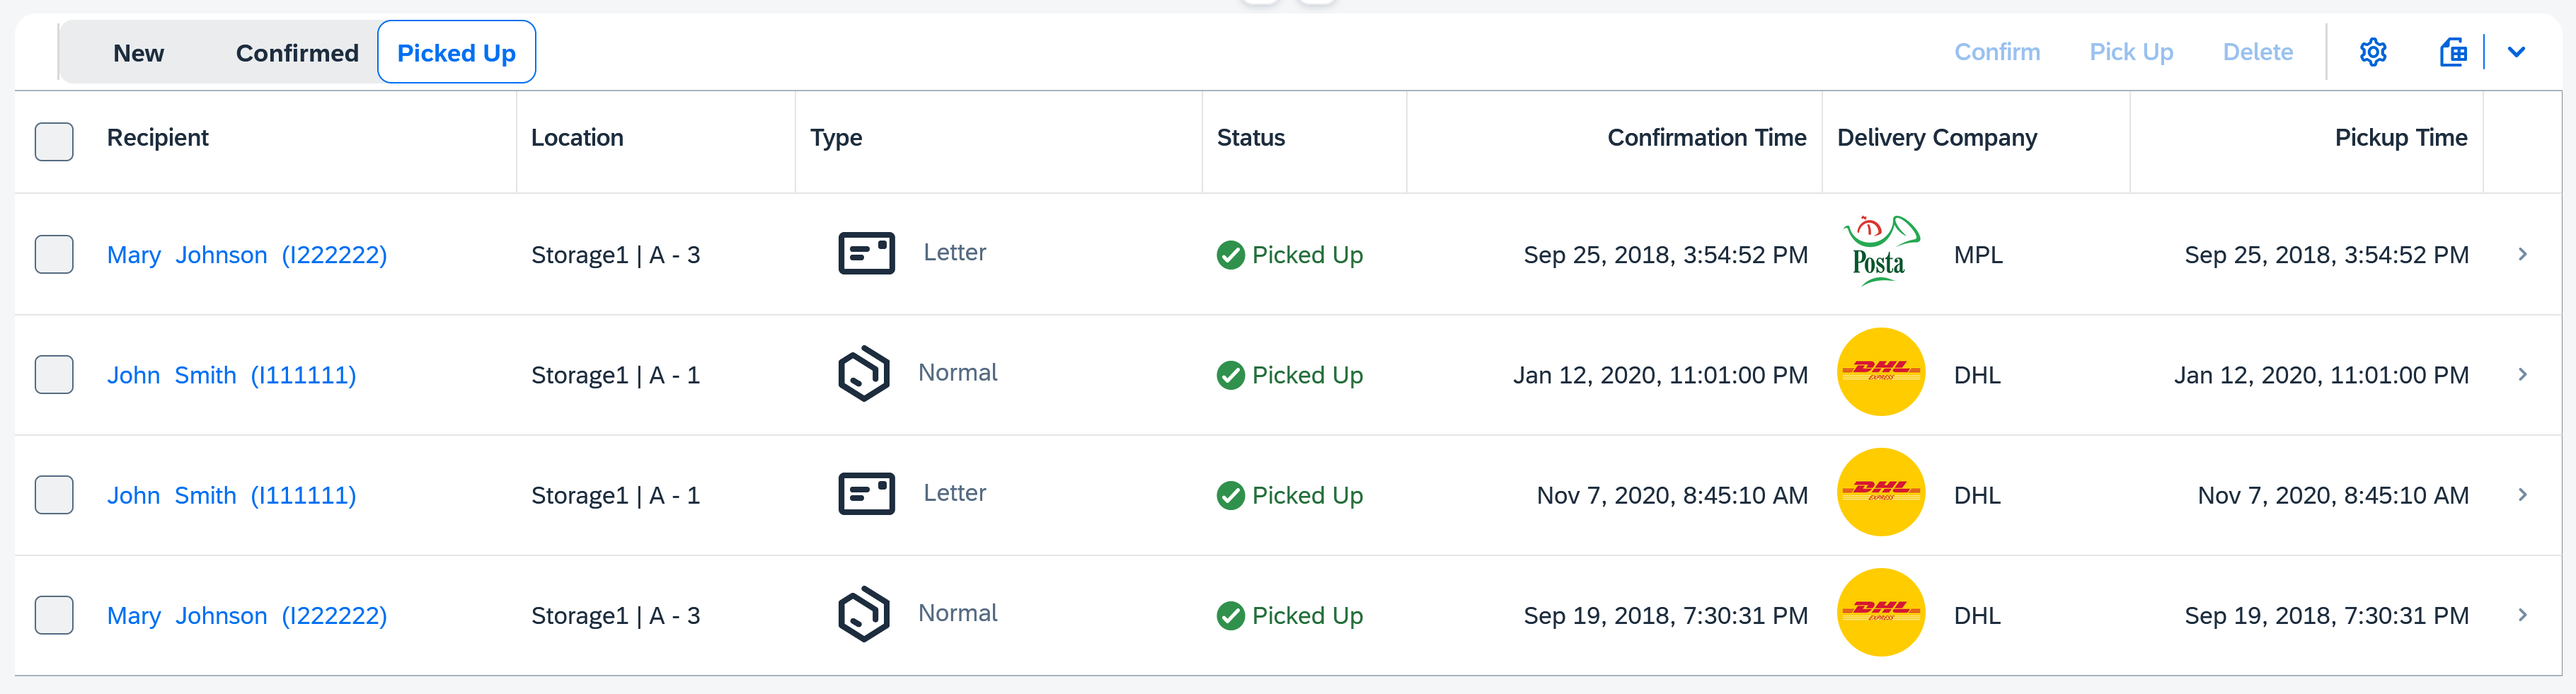
\includegraphics[width=0.85\linewidth]{images/user_doc/managePack/ReportScreen/browse/pickedupVariant.png}}
	\caption{Manage Packages Report Screen - Middle Control - Breadcrumb Show Case}
	\label{fig:MPBreadCrumb}
\end{figure}

A list of packages is displayed at the lower part. The information provided for each packages are: \textbf{Recipient} (the recipient info, full name and SAP ID), \textbf{Location} (the storage and storage slot info of the package, if applicable), \textbf{Type} (the type of the package, existing types are newspaper, letter and normal), \textbf{Status} (the status of the package, existing status are new, confirmed and picked up), \textbf{Delivery Company} (the delivery company of the package), \textbf{Confirmation Time} (the confirmation time of the package, if applicable), \textbf{Pickup Time} (the picked up time of the package, if applicable).

A package can be selected by ticking the selection box before the listed package item. A receptionist can also select and de-select all packages by toggling the selection box at the left corner of the list header (\autoref{fig:MPListSelection}).
By clicking on the \textbf{recipient} column item, a contact card will pop up displaying  the email and phone number of the recipient (\autoref{fig:MPReportCOntactCard}).

\bigskip
\begin{figure}[htb!]
	\centering
	\subcaptionbox{Select All}{
		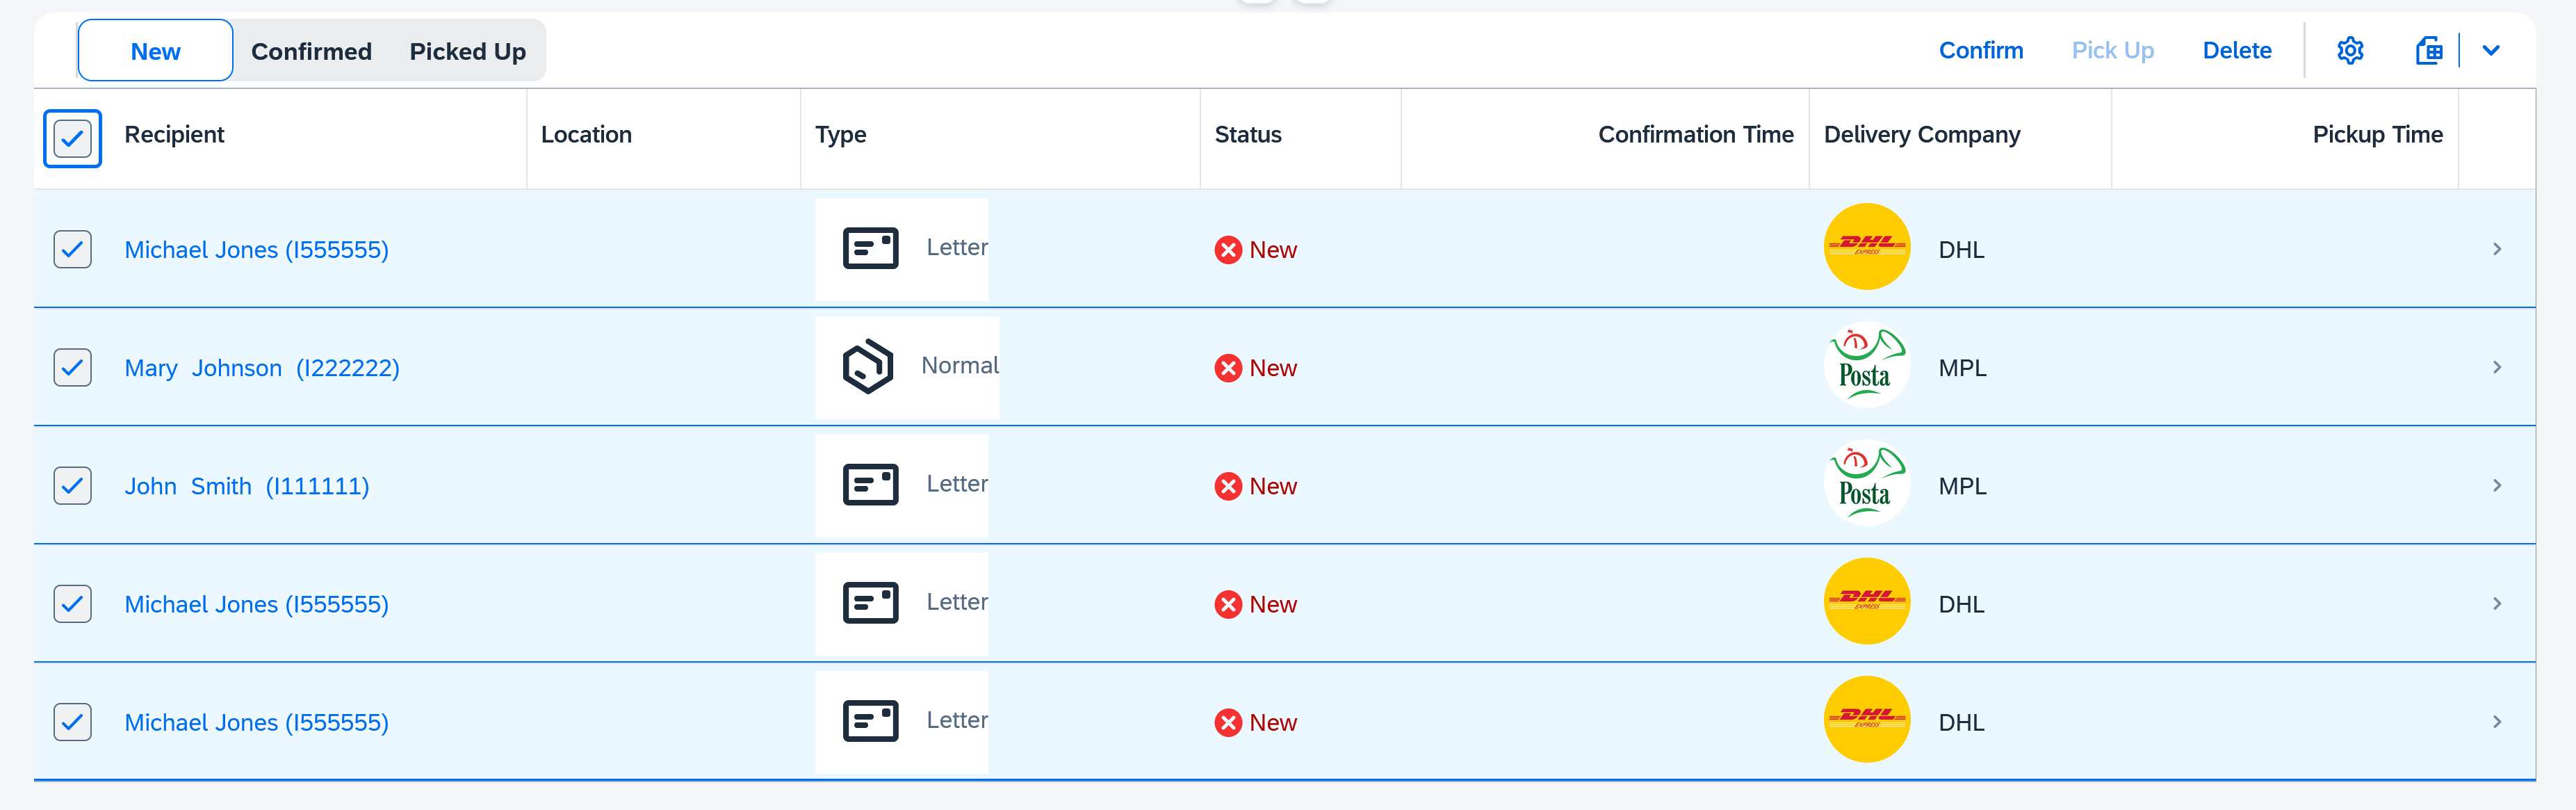
\includegraphics[width=0.95\linewidth]{images/user_doc/managePack/ReportScreen/browse/listSelectAll.png}}
  
	\vspace{10pt}
	\subcaptionbox{Deselect All}{
		\includegraphics[width=0.95\linewidth]{images/user_doc/managePack/ReportScreen/browse/listDeSelectAll.png}}
    \caption{Manage Packages Report Screen - Report List - Selection Show Case}
	\label{fig:MPListSelection}
\end{figure}

\begin{figure}[htb]
	\centering
	\includegraphics[height=200pt]{images/user_doc/managePack/ReportScreen/browse/contactcard.png}
	\caption{Manage Packages Report Screen - Report List - Contact Card Show Case}
	\label{fig:MPReportCOntactCard}
\end{figure}

Further details of a package can be obtained by clicking at the package list items. On clicking, the receptionist is navigated to the "Package Detail Screen" displaying \textbf{Basic}, \textbf{General Data} and \textbf{Administrative Data} of the package (\autoref{fig:MPdetailOverview}). 
A contact card can be displayed by clicking on the person fields (\autoref{fig:MPObjectContactCard}). 

\begin{figure}[H]
	\centering
	\includegraphics[width=1\linewidth]{images/user_doc/managePack/DetailScreen/browse/overview.png}
	\caption{Manage Packages Detail Screen - Overview}
	\label{fig:MPdetailOverview}
\end{figure}

\begin{figure}[H]
	\centering
	\subcaptionbox{Receptionist}{
		\includegraphics[width=0.48\linewidth]{images/user_doc/managePack/DetailScreen/browse/contactcard_recep.png}}
	\hspace{2pt}
	\subcaptionbox{Recipient}{
		\includegraphics[width=0.48\linewidth]{images/user_doc/managePack/DetailScreen/browse/contactcard_user.png}}
    \caption{Manage Packages Detail Screen - Contact Card}
	\label{fig:MPObjectContactCard}
\end{figure}

\subsubsection{Confirm Packages}

Confirming a package happens after a \textbf{Receptionist} registered a delivered package, when the \textbf{Receptionist} would like to allocate the package a storage slot. Only packages with \textit{new} status can be confirmed. One or more \textit{new} packages can be confirmed at a single time.

The \textbf{Confirm} button at the middle control part is used to trigger the confirm action. It is deactivated until at least one \textit{new} package is selected.
Once the \textbf{Receptionist} selected the packages (\autoref{fig:MPReportConfirmBtn}), the \textbf{Confirm} button is activated and clicked, a dialog pops up for the \textbf{Receptionist} to allocate a slot for the package(s) (\autoref{fig:MPReportConfirmDlg}). 

The storage should be selected first from the \textbf{Storage} drop down list and after that the \textbf{Slot} drop down list. The \textbf{Slot} drop down shows always the available slots under the selected storage (\autoref{fig:MPReportConfirmDlgSelection}).

After selecting the slot, if "Close" is clicked, nothing will happen and the dialog will be closed. If "Save" is clicked, the packages will be confirmed (i.e. filled with the selected slot info and status changed to confirmed). The dialog will be closed, a message toast indicates the success confirm and the package(s) will be moved from the current \textbf{New} variant to \textbf{Confirmed} Variant (\autoref{fig:MPReportConfirmDlgButton}).

At this point, the package(s) are ready to be picked up, by employee through \textbf{Package Pickup} (\autoref{subsec:pp}) application or by \textbf{Receptionist} using the pickup backup function (\autoref{subsubsec:MPpickup}) of this application.

\bigskip
Note that the confirm action is not irreversible, i.e. a \textit{confirmed} package can no longer be reset to \textit{new} and the confirmed package location can no longer be changed.

\bigskip
\begin{figure}[H]
	\centering
	\includegraphics[width=1\linewidth]{images/user_doc/managePack/ReportScreen/browse/confirmActivated.png}
	\caption{Manage Packages Report Screen - Confirm Step 1 - Select Packages}
	\label{fig:MPReportConfirmBtn}
\end{figure}

\begin{figure}[H]
	\centering
	\includegraphics[height=150pt]{images/user_doc/managePack/ReportScreen/confirm/confirmDialog.png}
	\caption{Manage Packages Report Screen - Confirm Step 2 - Confirm Dialog}
	\label{fig:MPReportConfirmDlg}
\end{figure}

\begin{figure}[H]
	\centering
	\subcaptionbox{Choose Storage}{
		\includegraphics[width=0.45\linewidth]{images/user_doc/managePack/ReportScreen/confirm/confirmStorageDropDown.png}}
	\hspace{5pt}
	\subcaptionbox{Choose Slot}{
		\includegraphics[width=0.45\linewidth]{images/user_doc/managePack/ReportScreen/confirm/confirmSlotDropdown.png}}
    \caption{Manage Packages Report Screen - Confirm Step 3 - Confirm Dialog - Location Selection}
	\label{fig:MPReportConfirmDlgSelection}
\end{figure}

\begin{figure}[H]
	\centering
	\subcaptionbox{Clicked "Save" and Proceeded}{
		\includegraphics[width=0.45\linewidth]{images/user_doc/managePack/ReportScreen/confirm/confirmedToast.png}}
	\hspace{5pt}
	\subcaptionbox{Clicked "Close" and Cancelled}{
		\includegraphics[width=0.45\linewidth]{images/user_doc/managePack/ReportScreen/browse/conifirmClosedClicked.png}}
    \caption{Manage Packages Report Screen - Confirm Step 4 - Confirmed / Cancelled}
	\label{fig:MPReportConfirmDlgButton}
\end{figure}

\subsubsection{Pickup Packages}
\label{subsubsec:MPpickup}

The Pickup of a package happens when the recipients (package owners) came to the reception trying to pickup their confirmed packages and they are unable to access the \textbf{Pickup Packages} application on their own. In this case a \textbf{Receptionist} may pickup the package on behalf of the recipients. Only packages with \textit{confirmed} status can be confirmed (learn more about the status of the packages in \autoref{sec:BusinessContext}). Only one \textit{confirmed} package at one time can be picked up.

The \textbf{Pickup} button at the middle control part is used to trigger the pickup action. It is deactivated until exactly one \textit{confirmed} package is selected at the \textbf{Confirmed} variant.

Once the \textbf{Confirm} button is activated (\autoref{fig:MPReportPickupBtn}) and clicked, a warning message box (\autoref{fig:MPReportPickupDlg}) pops up verifying the \textbf{Receptionist}'s intention to mark a package as pickup. If "OK" is clicked, the packages will be picked up (i.e. status is changed to pickup, all related processes are closed, package logs can no longer be removed from the system). The dialog will be closed, a message toast indicates the success of pickup and the package will be moved from the current \textbf{Confirmed} variant to \textbf{Picked Up} Variant (\autoref{fig:MPReportPickupDlgButton}). 

\bigskip
Note that the confirm action is not irreversible, i.e. a \textit{picked up} package can no longer be reset to \textit{confirm} or \textit{new}. However, the picked up package's information can still be modified (see \autoref{subsubsec:MPedit}).

\begin{figure}[H]
	\centering
	\includegraphics[width=1\linewidth]{images/user_doc/managePack/ReportScreen/pickup/pickupEnabled.png}
	\caption{Manage Packages Report Screen - Pickup Step 1 - Select Packages}
	\label{fig:MPReportPickupBtn}
\end{figure}

\begin{figure}[H]
	\centering
	\includegraphics[height=120pt]{images/user_doc/managePack/ReportScreen/pickup/pickupDialogOk.png}
	\caption{Manage Packages Pickup Dialog - Pickup Step 2}
	\label{fig:MPReportPickupDlg}
\end{figure}

\begin{figure}[H]
	\centering
	\subcaptionbox{Clicked "OK" and Proceeded}{
		\includegraphics[width=0.95\linewidth]{images/user_doc/managePack/ReportScreen/pickup/pickupToast.png}}
  
	\vspace{10pt}
	\subcaptionbox{Clicked "Cancel" and Cancelled}{
		\includegraphics[width=0.95\linewidth]{images/user_doc/managePack/ReportScreen/pickup/pickupCanceled.png}}
    \caption{Manage Packages Report Screen - Pickup Step 3 - Pickup / Cancelled}
	\label{fig:MPReportPickupDlgButton}
\end{figure}

\subsubsection{Delete Packages}

Deleting a package can be done in two ways: by batch deletions at the "Report Screen" or by single deletion at "Detail Screen". Only packages with \textit{confirmed} or \textit{new} status can be deleted. Packages with \textit{picked up} status can no longer be removed. Note that the deletion action is not irreversible.

In case the \textbf{Receptionist} is at "Report Screen" and he needs to delete some packages, the 
"Delete" button of the middle control bar should be used. The "Delete" button is deactivated until at least one package with \textit{Confirmed} or \textit{New} status is selected. Note that the \textit{New} and \textit{Confirmed} packages cannot be selected together at a single time. (See \autoref{sec:BusinessContext} for more information on the package status.)

Once the \textbf{Delete} button is activated (\autoref{fig:MPReportDeleteBtn}) and clicked, a warning message box (\autoref{fig:MCReportDeleteDlg}) pops up verifying the \textbf{Receptionist}'s intention to delete a package. 

If one "OK" is clicked, the packages will be deleted (i.e. the package no longer exists in the system). The message box will be closed, a message toast indicates the success of deletion and the package will be removed from everywhere. If "Cancel" is clicked, the message box is closed and nothing happens (\autoref{fig:MPReportDeleteDone}). 

\begin{figure}[H]
	\centering
	\subcaptionbox{Enabled}{
		\includegraphics[width=0.95\linewidth]{images/user_doc/managePack/ReportScreen/delete/deleteEnabled.png}}

	\subcaptionbox{Disabled for Picked Up Packages}{
		\includegraphics[width=0.95\linewidth]{images/user_doc/managePack/ReportScreen/delete/deleteDisabled.png}}
    \caption{Manage Packages Report Screen - Delete Step 1 - Select Packages}
	\label{fig:MPReportDeleteBtn}
\end{figure}

\begin{figure}[H]
	\centering
	\includegraphics[height=110pt]{images/user_doc/managePack/ReportScreen/delete/deleteDlalog.png}
	\caption{Manage Packages Delete Dialog - Delete Step 2}
	\label{fig:MPReportDeleteDlg}
\end{figure}

\begin{figure}[H]
	\centering
	\includegraphics[height=110pt]{images/user_doc/managePack/ReportScreen/delete/deleteToast.png}
	\caption{Manage Packages Delete Dialog - Delete Step 3 - Deleted}
	\label{fig:MPReportDeleteDone}
\end{figure}


\bigskip
In case the \textbf{Receptionist} is at "Detail Screen" and wants to delete the displayed package, the "Delete" button at the top right corner (page header) shall be used. 
The "Delete" button is activated if the displayed package is in the status \textbf{new} or \textbf{confirmed}.

If the "Delete" button is activated and clicked, a warning message box pops up verifying the \textbf{Receptionist}'s intention to delete the displayed package. If "Delete" is clicked, the packages will be deleted (i.e. the package no longer exist in the system). The message box will be closed, \textbf{Receptionist} got navigated back to "Report Screen" and a message toast indicates the success deletion. The package will be removed from everywhere. If "Cancel" is clicked, the message box is closed and nothing happens (\autoref{fig:MPDetailDeleteGuide}).

\begin{figure}[H]
	\centering
    \vspace{5pt}
	\subcaptionbox{Step 1: Deletion Enabled for Non-picked Up Packages}{
		\includegraphics[width=0.95\linewidth]{images/user_doc/managePack/DetailScreen/delete/deleteEnabled2.png}}
  
    \vspace{10pt}
	\subcaptionbox{Step 2: Deletion Verification}{
		\includegraphics[height=110pt]{images/user_doc/managePack/DetailScreen/delete/deleteDialog2.png}}
  
    \vspace{10pt}
    \subcaptionbox{Step 3: Navigated Back}{
		\includegraphics[width=0.95\linewidth]{images/user_doc/managePack/ReportScreen/delete/deleteToast.png}}
    \caption{Manage Packages Detail Screen - Delete Package Guide}
	\label{fig:MPDetailDeleteGuide}
\end{figure}

\subsubsection{Edit Packages}
\label{subsubsec:MPedit}

Editing a package can be done by the \textbf{Receptionist} at "Detail Screen" using the "Edit" button at top right corner (page header).
When the "Edit" button is clicked, an editing dialog pops up, allowing \textbf{Receptionist} to modify the \textbf{Recipient}, \textbf{Type}, \textbf{Delivery Company}, \textbf{Comment} of the package (\autoref{fig:MPDetailEditBtn}). 
When clicking "Save", the modified details are submitted, the dialog closes, a message toast pops up indicating the success and the changes reflects on the "Detail Screen". When clicking "Close", any changes will be discarded, the dialog is simply closed (\autoref{fig:MPReportEditDone}).

\begin{figure}[htb!]
	\centering
    \vspace{5pt}
	\subcaptionbox{Step 1: Edit Dialog}{
		\includegraphics[width=0.45\linewidth]{images/user_doc/managePack/DetailScreen/edit/editDialog.png}}
    \hspace{5pt}
    \subcaptionbox{Step 2: Modify Recipient}{
		\includegraphics[width=0.45\linewidth]{images/user_doc/managePack/DetailScreen/edit/editSelection1.png}}
	\subcaptionbox{Step 3: Modify Type}{
		\includegraphics[width=0.45\linewidth]{images/user_doc/managePack/DetailScreen/edit/editSelection2.png}}
    \hspace{5pt}
    \subcaptionbox{Step 4: Modify Delivery Company}{
		\includegraphics[width=0.45\linewidth]{images/user_doc/managePack/DetailScreen/edit/editSelection3.png}}
    \caption{Manage Packages Detail Screen - Edit Dialog Guide}
	\label{fig:MPDetailEditBtn}
\end{figure}

\begin{figure}[H]
	\centering
	\includegraphics[width=1\linewidth]{images/user_doc/managePack/DetailScreen/edit/editToast.png}
	\caption{Manage Packages Detail Screen - Edited}
	\label{fig:MPReportEditDone}
\end{figure}

%\pagebreak

\section{Facility Manager}
\label{sec:UdocFacilityManager}

The \textbf{Facility Manager} (See \autoref{sec:GeneralRequisite} for all possible roles) is granted to access the two applications under the \textbf{Administration} section, namely \textbf{Manage Companies} (\autoref{subsec:mc}) and \textbf{Manage Storage} (\autoref{subsec:ms}). 
A facility manager can quick jump to the section by left clicking the "Administration" tab. The application can be entered by left clicking the tiles (\autoref{fig:ManagerApplications}).

\begin{figure}[H]
	\centering
	\includegraphics[width=1\linewidth]{images/user_doc/overviews/AdminTab.png}
	\caption{Facility Management Applications}
	\label{fig:ManagerApplications}
\end{figure}


\subsection{Manage Companies}
\label{subsec:mc}

The \textbf{Manage Companies} application is used by \textbf{Facility Manager} (in short \textbf{FM}) to maintain the information in the system of potential companies delivering packages. For each delivery company, its name, optionally a logo and the administration data (creation time, creation user, last modified time, last modified user) are stored. The administration data are auto maintained and are not editable by the \textbf{FM}. The reader can navigate to \autoref{subsec:dev-ui-mc} for more implementation details. The summarized main actions the \textbf{FM} can take within the application are listed:

\begin{compactenum}
	\item Browse the delivery companies.
        \begin{compactenum}
            \item Filtering possibility.
            \item Report List of delivery companies info.
            \item Detail page for single delivery company.
        \end{compactenum}
    \item Add new delivery companies. (name and logo)
    \item Edit existing delivery companies (name and logo).
    \item Delete package(s) which status is new or confirmed.
\end{compactenum}

\subsubsection{Browse Companies}
A Facility Manager \textbf{FM}, after clicking on the application tile, is redirected to the "Report Screen", which is the main screen of the application (\autoref{fig:CompanyOverview}). 

\begin{figure}[H]
	\centering
	\includegraphics[width=1\linewidth]{images/user_doc/company/report/overview.png}
	\caption{Manage Companies - Overview}
	\label{fig:CompanyOverview}
\end{figure}

The upper part displays the search bar and the possible filters. 
The \textbf{"Search Bar"} can be used in case of the need of searching for an item with free text. The search supports in-completed keywords and is case insensitive. The fixed filters can also be used for administration data. "Created By" and "Last Updated By" accepts free text of any valid SAP ID. "Created On" and "Last Updated On" requires entries of time stamps. The double square at the right of input bar can be clicked to open a filter help dialog, where specific criteria (e.g. between, equal, contains, etc.) can be chosen and a time entry clock can be used to enter time stamps (\autoref{fig:CompanyOverview}). 

When adjusting the filtering values, the list view is temporarily locked. By clicking the "Go" button or hit "Enter" on keyboard, the filters are run and result can be reviewed. In case a company is edited and the table content is not reflected, it can be refreshed by clicking the "Go" button or hitting "Enter" on keyboard (\autoref{fig:CompanyOverview}). 

The lower part displays the list of delivery companies. In the list header, number of total delivery companies in the list is displayed on the left and two action buttons, "Create" and "Delete" are placed on the right (\autoref{fig:CompanyOverview}). 

The information provides for each delivery companies in the list body (table) are: \textbf{Delivery Company} (company name with logo), \textbf{Created On} (the creation time of the company), \textbf{Created By} (the company creator's SAP ID) (\autoref{fig:CompanyOverview}). 

A package can be selected by ticking the selection box before the listed package item. A facility manager can also deselect all packages at once by clicking at the selection box at the left corner of the table header (\autoref{fig:CompanyOverview}). 

\bigskip

When the \textbf{FM} clicks on one item of the table, the \textbf{FM} is redirected to the "Detail Screen" which displays the details of the selected item (\autoref{fig:MCdetailOVerview}). 

\begin{figure}[H]
	\centering
	\includegraphics[width=1\linewidth]{images/user_doc/company/detail/DetailOverview.png}
	\caption{Manage Company Detail Screen - Overview}
	\label{fig:MCdetailOVerview}
\end{figure}

The "Detail Screen" displays the company name as the title on the left and two action buttons, "Delete" and "Edit" at the right in the header, and its full administration data in the body (\autoref{fig:MCdetailOVerview}). 

\subsubsection{Add Company}

A new delivery company can be added to the system at "Report Screen" by clicking the "Create" button. 
A creation dialog pops up when the "Create" button is clicked, where the \textbf{Name} and the \textbf{Logo} info of the company should be entered. The \textbf{Name} waits for input of free text of the company name and should not be left empty. The \textbf{Logo} waits for input of free text of a url to the image of the company's logo and can be left empty (\autoref{fig:MCreportCreateGuide} - a,b). 

After filling the dialog form, if "Create" is clicked, the entered info will be submitted, the dialog will be closed, a success message toast is displayed and the entered company appears in the table on the "Report Screen". If "Cancel" is clicked, the dialog will be closed, entered data is discarded and nothing happens (\autoref{fig:MCreportCreateGuide} - c).

\begin{figure}[H]
	\centering
	\subcaptionbox{Step 1: Create Dialog}{
		\includegraphics[width=0.45\linewidth]{images/user_doc/company/report/createDlg.png}}
    \hspace{5pt}
    \subcaptionbox{Step 2: Data Entry}{
		\includegraphics[width=0.45\linewidth]{images/user_doc/company/report/createDlgEntries.png}}
    \vspace{10pt}
   \subcaptionbox{Step 3: Post Creation}{
		\includegraphics[width=0.95\linewidth]{images/user_doc/company/report/createdToast.png}}
    \caption{Manage Company Report Screen - Create Dialog Guide}
	\label{fig:MCreportCreateGuide}
\end{figure}

\subsubsection{Edit Company}

A delivery company can be edited at "Detail Screen" by the \textbf{FM} using the "Edit" button at top right corner (page header). 
When the "Edit" button is clicked, an editing dialog pops up, allowing \textbf{FM} to modified the \textbf{Name}, \textbf{Logo} of the company. Initially the fields are filled with current data of the company. The \textbf{Name} should contain free text of the company's name and should not be left empty. The \textbf{Logo} should contain free text of a url to the logo image and can be left empty.
When "Save" is clicked, the modified details are submitted, the dialog closes, a message toast pops up indicating the success and the changes are reflected on the "Detail Screen". When clicking "Close", any changes will be discarded, the dialog simply closes (\autoref{fig:MCDetailEditGuide}, \autoref{fig:MCDetailEditDlgBad}). 

\begin{figure}[H]
	\centering
    \vspace{5pt}
	\subcaptionbox{Step 1: Edit Dialog}{
		\includegraphics[width=0.35\linewidth]{images/user_doc/company/detail/EditDlg.png}}
    \hspace{5pt}
    \subcaptionbox{Step 2: Post Success Edit}{
		\includegraphics[width=0.55\linewidth]{images/user_doc/company/detail/EditToast.png}}
    \caption{Manage Company Detail Screen - Edit Dialog Guide}
	\label{fig:MCDetailEditGuide}
\end{figure}

\begin{figure}[H]
	\centering
    \vspace{5pt}
	\subcaptionbox{Empty Company Name}{
		\includegraphics[width=0.35\linewidth]{images/user_doc/company/detail/EditBadInput.png}}
    \hspace{5pt}
    \subcaptionbox{Step 2: Error Message}{
		\includegraphics[width=0.55\linewidth]{images/user_doc/company/detail/editBadInputErrorMsg.png}}
    \caption{Manage Companies Detail Screen - Edit Dialog - Bad Inputs Example}
	\label{fig:MCDetailEditDlgBad}
\end{figure}

\subsubsection{Delete Company}

Deleting an existing delivery company can be done in two ways: batch deletions at the "Report Screen" or single deletion at "Detail Screen". The deletion of a company implies that, the delivery company will be removed completely and any association of existing packages to this company is automatically removed as well. This means those packages will no longer hold any company information. The deleting action is irreversible. 

In case the \textbf{FM} is at "Report Screen", one or more companies can be deleted using the "Delete" button at the list header. The "Delete" button is deactivated until at least one delivery company is selected.

Once the \textbf{Delete} button is activated and clicked, a warning message box pops up verifying the \textbf{FM}'s intention to delete a package. If "OK" is clicked, the company(s) will be deleted. The message box will be closed, a message toast indicates the success deletion and the package will be removed from everywhere. If "Cancel" is clicked, the message box is closed and nothing happens (\autoref{fig:MCReportDeleteStep1}, \autoref{fig:MCReportDeleteDlg}, 
\autoref{fig:MCReportDeleteStep3}).


\begin{figure}[H]
	\centering
	\includegraphics[width=0.90\linewidth]{images/user_doc/company/report/deleteBtnEnable.png}
	\caption{Manage Companies - Delete - Step 1: Select Company to Delete}
	\label{fig:MCReportDeleteStep1}
\end{figure}

\begin{figure}[H]
	\centering
	\includegraphics[height=100pt]{images/user_doc/company/report/deleteConfirmaton2.png}
	\caption{Manage Companies - Delete - Step 2: Delete Dialog}
	\label{fig:MCReportDeleteDlg}
\end{figure}

\begin{figure}[H]
	\centering
	\includegraphics[width=0.90\linewidth]{images/user_doc/company/report/deleteToast.png}
	\caption{Manage Companies - Delete - Step 3: Post Delete}
	\label{fig:MCReportDeleteStep3}
\end{figure}

\bigskip
In case the \textbf{FM} is at "Detail Screen" and want to delete the displayed company, the "Delete" button at the top right corner (page header) should be used. 

Once clicked, a warning message box pops up verifying the \textbf{FM}'s intention to delete the displayed company. If "Delete" is clicked, the company will be deleted. The message box will be closed, \textbf{FM} got navigated back to "Report Screen" and a message toast indicates the success deletion. If "Cancel" is clicked, the message box is closed and nothing happens (\autoref{fig:MCDetailDeleteGuide}).

\bigskip
\begin{figure}[htb!]
	\centering
	\subcaptionbox{Step 1: Deletion Verification When Clicked "Delete"}{
		\includegraphics[width=0.95\linewidth]{images/user_doc/company/detail/deleteConfirmation.png}}
  
    \vspace{10pt}
	\subcaptionbox{Step 2: Navigated Back After Deletion}{
		\includegraphics[width=0.99\linewidth]{images/user_doc/company/detail/AfterDeletionBack.png}}
    \caption{Manage Companies Detail Screen - Delete Company Guide}
	\label{fig:MCDetailDeleteGuide}
\end{figure}



\subsection{Manage Storage}
\label{subsec:ms}

The \textbf{Manage Storage} application is used by \textbf{Facility Manager} (in short \textbf{FM}) maintaining the information of potential storage places and storage slots within certain storage holding the package in the system (see \autoref{sec:UdocFacilityManager} for all facility manager related applications). The reader can navigate to \autoref{subsec:dev-ui-ms} for more implementation details. 

\bigskip
\noindent
List of the summarized main actions the \textbf{FM} can take within the application:
\begin{compactenum}
	\item Browse the storage and slots in the storage.
        \begin{compactenum}
            \item Filtering possibility.
            \item Report List of storage.
            \item Detail page for storage.
            \item Detail page for slot.
        \end{compactenum}
    \item Add new storage.
        \begin{compactenum}
            \item At Storage Report Page.
        \end{compactenum}
    \item Edit existing storage.
        \begin{compactenum}
            \item At Storage Detail Page.
        \end{compactenum}
    \item Delete existing storage.
        \begin{compactenum}
            \item At Storage Report Page.
            \item At Storage Detail Page.
        \end{compactenum}
    \item Add new storage slot.
        \begin{compactenum}
            \item At Storage Detail Page.
        \end{compactenum}
    \item Batch add new storage slots.
        \begin{compactenum}
            \item At Storage Detail Page.
        \end{compactenum}
    \item Edit existing storage slot.
        \begin{compactenum}
            \item At Slot Detail Page.
        \end{compactenum}
    \item Delete existing storage slot.
        \begin{compactenum}
            \item At Slot Detail Page.
            \item At Storage Detail Page.
        \end{compactenum}
\end{compactenum}

\subsubsection{Browse}

An \textbf{FM}, after clicking at the application tile, it is redirected to the "Storage Report Screen", which is the main screen of the application (\autoref{fig:MSstorageReportPage}). 

\begin{figure}[H]
	\centering
	\includegraphics[width=1\linewidth]{images/user_doc/storage/StorageReportPage/reportDefaultOverview.png}
	\caption{Manage Storage - Storage Report Screen}
	\label{fig:MSstorageReportPage}
\end{figure}

The upper part displays the search bar and the possible filters. 
The \textbf{"Search Bar"} can be used in case of the need of searching for an item with free text. The search supports incompleted keywords and it is case insensitive.
A facility manager \textbf{FM} can also use the default filters, "Building Floor" and "Building", which are two drop down of all available building floors and buildings. A facility manager \textbf{FM} may use the "Adapt Filter" option (right most of the filter bar), through which more filters options can be added onto the filter bar (\autoref{fig:MSstReportFilterBar}, 
\autoref{fig:MSstorageReportFilterDefault}, 
\autoref{fig:MSstorageReportFilterAdaption}).

\bigskip
\begin{figure}[htb]
	\centering
	\includegraphics[width=1\linewidth]{images/user_doc/storage/StorageReportPage/reportFilterBar.png}
	\caption{Manage Storage Storage Report Screen - Filter Bar}
	\label{fig:MSstReportFilterBar}
\end{figure}

\begin{figure}[htb]
	\centering
	\subcaptionbox{Drop Down of All Possible Building Floor Options}{
		\includegraphics[width=0.5\linewidth]{images/user_doc/storage/StorageReportPage/defaultFIlterBF.png}}
  
    \vspace{10pt}
    \subcaptionbox{Drop Down of All Possible Building Options}{
		\includegraphics[width=0.5\linewidth]{images/user_doc/storage/StorageReportPage/defaultFIlterBD.png}}
    \caption{Manage Storage Storage Report Screen - Filter Drop down Show Case}
	\label{fig:MSstorageReportFilterDefault}
\end{figure}

\begin{figure}[htb]
	\centering
	\subcaptionbox{Option Dialog 1: Simple List}{
		\includegraphics[width=0.45\linewidth]{images/user_doc/storage/StorageReportPage/filterOption.png}}
    \hspace{5pt}
    \subcaptionbox{Option Dialog 2: Grouped}{
		\includegraphics[width=0.45\linewidth]{images/user_doc/storage/StorageReportPage/filterOption2.png}}

    \vspace{10pt}
	\subcaptionbox{After Filter Adaption}{
		\includegraphics[width=1\linewidth]{images/user_doc/storage/StorageReportPage/filterAdaption.png}}
    \caption{Manage Storage Storage Report Screen - Filter Adaption Guide}
	\label{fig:MSstorageReportFilterAdaption}
\end{figure}

When adjusting the filtering values, the list view is temporarily locked. The filter can be run by clicking the "Go" button or hit "Enter" on keyboard. The "Go" button or the "Enter" on keyboard can be used to refresh the table in case a storage is edited or deleted and the table content is not reflected (\autoref{fig:MSstorageReportFilterLock}). 


\begin{figure}[!htb]
	\centering
    \vspace{5pt}
	\subcaptionbox{While Adjusting the Filters the Storage List is Locked}{
		\includegraphics[width=0.7\linewidth]{images/user_doc/storage/StorageReportPage/listLock.png}}
    
    \vspace{10pt}
    \subcaptionbox{Clicked "Go" to Display the Filtering Results}{
		\includegraphics[width=0.7\linewidth]{images/user_doc/storage/StorageReportPage/filterAfterGo.png}}
    \caption{Manage Storage Storage Report Screen - Filter Lock}
	\label{fig:MSstorageReportFilterLock}
\end{figure}

\bigskip

The lower part displays the list report of storage. In the list header, the number of total storage of the list is displayed on the left and two action buttons, "Create" and "Delete", and a table column "setting" (icon) are placed on the right (\autoref{fig:MSrl}).

The default columns provided for each storage in the list body (table) are: \textbf{Name} (storage name), \textbf{Location} (the building floor the storage located on), \textbf{Location Instructions} (any helping info regarding the location of the storage), \textbf{Total Number of Packages} (the total number of the packages that had been confirmed in this storage since its creation), \textbf{Current Utilizations} (the number of packages that are currently confirmed in this storage), \textbf{Map} (a link, on click opens a new tab to the map of the location of the storage) (\autoref{fig:MSrl}). 


More columns may be displayed in the table by clicking the "setting" icon on the list header. A column adaption dialog will pop up for the \textbf{FM} to select the columns to show (\autoref{fig:MSstorageReportColumnAdaption}).


\begin{figure}[!htb] % Storage List
	\centering
	\includegraphics[width=0.99\linewidth]{images/user_doc/storage/StorageReportPage/reportList.png}
	\caption{Manage Storage Storage Report Screen - Storage List}
	\label{fig:MSrl}
\end{figure}

\begin{figure}[htb] % MSstorageReportColumnAdaption
	\centering
	\subcaptionbox{Step 1: column "setting"}{
		\includegraphics[width=0.45\linewidth]{images/user_doc/storage/StorageReportPage/columnSettings.png}}
    \hspace{5pt}
	\subcaptionbox{Step 2: Column Selection Dialog}{
		\includegraphics[width=0.45\linewidth]{images/user_doc/storage/StorageReportPage/columnAdaptionDlg.png}}
    
    \vspace{10pt}
    \subcaptionbox{Step 3: Selected Columns Displayed}{
        \includegraphics[width=0.95\linewidth]{images/user_doc/storage/StorageReportPage/columnMOre.png}}
    \caption{Manage Storage Storage Report Screen - Column Adaption Guide}
	\label{fig:MSstorageReportColumnAdaption}
\end{figure}

A storage can be selected by ticking the selection box before the listed storage item. A facility manager may also deselect all storage by clicking at the selection box at the left corner of the table header.

%\bigskip

When clicking at a row of the table, the \textbf{FM} is redirected to the "Storage Detail Screen" (\autoref{fig:MSdetailOVerview}).


\begin{figure}[H]
	\centering
	\includegraphics[width=1\linewidth]{images/user_doc/storage/updatedSlotEditDelete/StorageObjectOverview.png}
	\caption{Manage Storage Storage Detail Screen - Overview}
	\label{fig:MSdetailOVerview}
\end{figure}

The header part of "Storage Detail Screen" displays the storage name as the title and location instruction as description on the left and two action buttons, "Delete" and "Edit" at the right.
Under the title the important info of the storage is displayed (location, total utilization, current utilization and map). On clicking the map, the \textbf{FM} will be redirected out of the application to the map of the storage (\autoref{fig:MSstorageObjHeader}).

\begin{figure}[!htb] % StorageObjHeader
	\centering
	\includegraphics[width=1\linewidth]{images/user_doc/storage/StorageObjectPage/StorageObjHeader.png}
	\caption{Manage Storage Storage Detail Screen - Header}
	\label{fig:MSstorageObjHeader}
\end{figure}

The bottom body part displays the list of slots contained by the given storage. 
The following columns / information are displayed in the list of slots: \textbf{Name} (slot name), \textbf{Total Number of Packages} (total number of the packages stored in the slot since its creation date), \textbf{status} (the status of the slot). The available status of the slot are: \textit{inuse} (indicates there is currently at least one package stored inside), \textit{empty} (indicates there is no package inside) and \textit{unavailable} (indicates the slot cannot be used due to some reasons).
The list table tool bar contains two action buttons: \textbf{Create} (\autoref{subsubsec:addSlot}) and \textbf{Mass Create} (\autoref{subsubsec:batchAddSlot}) for single and batch creation of the slot. 
At the end of each line items two (or one depends on the status) actions buttons are displayed for the edition (\autoref{subsubsec:editSlot}) and deletion (\autoref{subsubsec:deleteSlot}) of the slot (\autoref{fig:MSstorageObjSlotList}).
In case a slot is edited or deleted and the table content is not reflected, refresh the entire page.

\begin{figure}[H] % slotList
	\centering
	\includegraphics[width=1\linewidth]{images/user_doc/storage/updatedSlotEditDelete/StorageObjectSlotTable.png}
	\caption{Manage Storage Storage Detail Screen - Slot List}
	\label{fig:MSstorageObjSlotList}
\end{figure}

\bigskip

\subsubsection{Add Storages}

New storages can be added to the system by the \textbf{FM} at "Report Screen" using the "Create" button.
A creation dialog pops up when the "Create" button is clicked. The \textbf{Name} field waits for input of free text of the storage and should not be left empty. The \textbf{Map} field waits for the input of free text of a url to the location of the storage and can be left empty.The free text input is required by the \textbf{Location Instruction} field and it can be left empty (\autoref{fig:MSreportCreateGuide1}).

After filling the dialog form, if "Create" is clicked, the entered info will be submitted, the dialog will be closed, a success message toast is displayed and the entered storage appears in the table on the "Report Screen". If "Cancel" is clicked, the dialog will be closed, the entered data is discarded and nothing happens (\autoref{fig:MSreportCreateGuide2}).


\begin{figure}[!htb]
    \centering
    \begin{subfigure}{0.45\linewidth}
        \includegraphics[width=\linewidth]{images/user_doc/storage/StorageReportPage/createStorageDlg.png}
        \caption{Step 1: Open Create Dialog}
    \end{subfigure}
    \hspace{5pt}
    \begin{subfigure}{0.4\linewidth}
        \includegraphics[width=\linewidth]{images/user_doc/storage/StorageReportPage/csdlgDropDown.png}
        \caption{Step 2.1: Data Entry - Select Building Floor}
    \end{subfigure}

    \begin{subfigure}{0.45\linewidth}
        \includegraphics[width=\linewidth]{images/user_doc/storage/StorageReportPage/csdlgBadInput.png}
        \caption{Step 2.2: Data Entry - Bad Input Warning Example}
    \end{subfigure}
    \hspace{5pt}
    \begin{subfigure}{0.45\linewidth}
        \includegraphics[width=\linewidth]{images/user_doc/storage/StorageReportPage/csdlgFilled.png}
        \caption{Step 2.2: Data Entry - Filled}
    \end{subfigure}

    
    \caption{Manage Storage Storage Report Screen - Create Storage Dialog Guide (Part 1)}
    \label{fig:MSreportCreateGuide1}
\end{figure}

\begin{figure}[H]
    \ContinuedFloat
    \centering
    
    \begin{subfigure}{0.95\linewidth}
        \includegraphics[width=\linewidth]{images/user_doc/storage/StorageReportPage/createdToast.png}
        \caption{Step 3: Post Creation}
    \end{subfigure}
    
    \caption{Manage Storage Storage Report Screen - Create Storage Dialog Guide (Part 2)}
    \label{fig:MSreportCreateGuide2}
\end{figure}

\subsubsection{Edit Storages}

A storage can be edited at "Storage Detail Screen" by the \textbf{FM} using the "Edit" button at top right corner (page header). 
When the "Edit" button is clicked, a editing dialog pops up, allowing the modification of the \textbf{Name}, \textbf{Building Floor}, \textbf{Map}, \textbf{Location Instructions} of the company. Initially the fields are filled with the current data of the storage. The entry rules are the same as creating a storage.
When clicking "Save", the modified details are submitted, the dialog is closed, a message toast is popped up indicating the success and the changes are reflected on the "Storage Detail Screen". If "Close" is clicked, any changes will be discarded and the dialog is simply closed (\autoref{fig:MSDetailEditBtn}).


\begin{figure}[H]
	\centering
    \vspace{5pt}
	\subcaptionbox{Step 1: Edit Dialog}{
		\includegraphics[width=0.50\linewidth]{images/user_doc/storage/StorageObjectPage/storageEditDlg.png}}
    \vspace{5pt}
    
    \subcaptionbox{Step 2: Post Success Edit}{
		\includegraphics[width=0.90\linewidth]{images/user_doc/storage/StorageObjectPage/storageEditedToast.png}}
    \caption{Manage Storage Storage Detail Screen - Edit Dialog Guide}
	\label{fig:MSDetailEditBtn}
\end{figure}

\subsubsection{Delete Storages}

Deleting a storage can be done in two ways: batch deletions at the "Storage Report Screen" or single deletion at "Storage Detail Screen". 
The deletion of a storage implies that, the storage will be removed completely from the system. The deletion action is irreversible. 

To delete a storage at "Storage Report Screen", the "Delete" button at the list header should be used. The "Delete" button is deactivated until at least one storage is selected and no storage containing slots that stores a package is selected.

Once the "Delete" button is activated and clicked, a warning message box pops up verifying the \textbf{FM}'s intention to delete a storage. If one more "Delete" is clicked, the selected storage will be deleted. The message box will be closed, a message toast is shown indicating the success deletion. If "Cancel" is clicked, the message box is closed and nothing happens (\autoref{fig:MSreportDeleteGuide}).

\begin{figure}[H]
	\centering
	\subcaptionbox{Step 1: Select Storage}{
		\includegraphics[width=0.95\linewidth]{images/user_doc/storage/StorageReportPage/deleteEnable.png}}
  
    \vspace{10pt}
    
    \subcaptionbox{Step 2: Delete Verification}{
		\includegraphics[width=0.45\linewidth]{images/user_doc/storage/StorageReportPage/deleteVerification.png}}
  
    \vspace{10pt}
    
    \subcaptionbox{Step 3: Deleted}{
		\includegraphics[width=0.95\linewidth]{images/user_doc/storage/StorageReportPage/deleteToast.png}}

    \caption{Manage Storage Storage Report Screen - Delete Storage Guide}
	\label{fig:MSreportDeleteGuide}
\end{figure}


%\bigskip
In case the \textbf{FM} is at "Storage Detail Screen", the "Delete" button at the top right corner (page header) can be used. 
Once clicked, a warning message box pops up verifying the \textbf{FM}'s intention to delete the displayed storage. If "Delete" is clicked, the storage will be deleted. The message box will be closed, the \textbf{FM} will be navigated back to "Storage Report Screen" and a message toast is shown indicating the success deletion. If "Cancel" is clicked, the message box is closed and nothing happens (\autoref{fig:MSobjDeleteGuide}).

\begin{figure}[H]
	\centering
	\subcaptionbox{On Click "Delete" - Deletion Verification}{
		\includegraphics[width=0.95\linewidth]{images/user_doc/storage/StorageObjectPage/storageDeleteMsg.png}}

    \caption{Manage Storage Storage Detail Screen - Delete Storage Guide}
	\label{fig:MSobjDeleteGuide}
\end{figure}


\subsubsection{Add Storage Slots}
\label{subsubsec:addSlot}

A new storage slot can be added to the system at "Storage Detail Screen" by clicking the "Create" button on the top right corner of the slot list.
When the "Create" button is clicked, a creation dialog pops up. The \textbf{Name} waits for input of free text of the storage slot and should not be left empty. The newly created slot can be marked as in unavailable status by deselecting the \textbf{Available} selection box (\autoref{fig:MSobjCreateSlotGuide1}).

After filling the dialog form, if "Create" is clicked, the entered info will be submitted, the dialog will be closed, a success message toast is displayed and the entered storage slot appears in the table on the "Storage Detail Screen". In case \textbf{Available} is selected, the created slot will by default of status "empty", otherwise, the status is set to "unavailable". If "Cancel" is clicked, the dialog will be closed, entered data is discarded and nothing happens (\autoref{fig:MSobjCreateSlotGuide2}).

\begin{figure}[htb]
    \centering
    \begin{subfigure}{0.45\linewidth}
        \includegraphics[width=\linewidth]{images/user_doc/storage/StorageObjectPage/createSlotDlg.png}
        \caption{Step 1: Open Create Dialog}
    \end{subfigure}
    \hspace{10pt}
    \begin{subfigure}{0.45\linewidth}
        \includegraphics[width=\linewidth]{images/user_doc/storage/StorageObjectPage/createSlotBadInput.png}
        \caption{Step 2: Data Entry - Bad Input Warning Example}
    \end{subfigure}

    \caption{Manage Storage Storage Detail Screen - Create Slot Dialog Guide (Part 1)}
    \label{fig:MSobjCreateSlotGuide1}
\end{figure}

\begin{figure}[htb]
    \ContinuedFloat
    \centering
    \begin{subfigure}{0.95\linewidth}
        \includegraphics[width=\linewidth]{images/user_doc/storage/updatedSlotEditDelete/singleSlotCreateToast.png}
        \caption{Step 3: Post Creation}
    \end{subfigure}
    
    \caption{Manage Storage Storage Detail Screen - Create Slot Dialog Guide (Part 2)}
    \label{fig:MSobjCreateSlotGuide2}
\end{figure}


\subsubsection{Batch Add Storage Slots}
\label{subsubsec:batchAddSlot}

Multiple new storage slots can be added at one time in a matrix way at "Storage Detail Screen" by clicking the "Mass Create" button on the top right corner of the slot list.
When the "Mass Create" button is clicked, a creation dialog pops up. Numeric integer inputs of desired number of rows and columns to create is required for the \textbf{Number of Rows} and \textbf{Number of Columns} fields. The \textbf{Type of Row Identifiers} and \textbf{Type of Column Identifiers} fields has two options: Number and Letter, indicates how the created matrix of slot will be named (Row - Column). If "Letter" is selected then "A-Z" will be used, otherwise, "1-9". For example, an entry of (1, Letter, 2, Number) will create (A - 1, A - 2). The selection of row and column type should not be the same (\autoref{fig:MSobjmassCreateSlotGuide}).

After filling the dialog form, if "Create" is clicked, the entered info will be submitted, the dialog will be closed, a success message toast is displayed and the created storage slots are shown in the table on the "Storage Detail Screen". If "Cancel" is clicked, the dialog will be closed, the entered data is discarded (\autoref{fig:MSobjmassCreateSlotGuide}).

\begin{figure}[htb!] % MSobjmassCreateSlotGuide
	\centering
	\subcaptionbox{Step 1: Open Create Dialog}{
		\includegraphics[width=0.45\linewidth]{images/user_doc/storage/StorageObjectPage/masCreateDlg.png}}

    \vspace{10pt}
    \subcaptionbox{Step 2.1: Data Entry - Row Type Selection}{
		\includegraphics[width=0.45\linewidth]{images/user_doc/storage/StorageObjectPage/massCreateFilling1.png}}
    \hspace{5pt}
    \subcaptionbox{Step 2.2: Data Entry - Column Type Selection}{
		\includegraphics[width=0.45\linewidth]{images/user_doc/storage/StorageObjectPage/massCreateFilling2.png}}

    \vspace{10pt}
    \subcaptionbox{Step 2.1: Data Entry - Row Type Selection}{
		\includegraphics[width=0.90\linewidth]{images/user_doc/storage/updatedSlotEditDelete/MassCreateToast.png}}
    \caption{Manage Storage Storage Detail Screen - Mass Create Slot Dialog Guide}
	\label{fig:MSobjmassCreateSlotGuide}
\end{figure}


\subsubsection{Edit Storage Slots}
\label{subsubsec:editSlot}
A slot can be edited at the "Storage Detail Screen" using the "Edit" (icon with pen) at the end of each slot row. 
When the "Edit" button is clicked, an editing dialog pops up, allowing the modification of the \textbf{Name}, \textbf{Available} of the slot. Initially the fields are filled with current data of the slot. The entry rules are the same as creating a single slot. Additionally, the \textbf{Available} selection box is non-editable if the slot is in \textit{inuse} status (\autoref{fig:MSSlotDetailEditBtn}/a).

If "Save" is clicked, the modified details are submitted, the dialog is closed, a message toast pops up indicating the success and the changes are reflected on the "Storage Detail Screen". If "Close" is clicked, any changes will be discarded, the dialog is simply closed (\autoref{fig:MSSlotDetailEditBtn}/b).

\begin{figure}[htb!]
	\centering
    \vspace{5pt}
	\subcaptionbox{Step 1: Edit Dialog}{
		\includegraphics[width=0.65\linewidth]{images/user_doc/storage/SlotObjectPage/editSlotDlg.png}}
    \vspace{10pt}
    
    \subcaptionbox{Step 2: Post Success Edit}{
		\includegraphics[width=0.95\linewidth]{images/user_doc/storage/updatedSlotEditDelete/updatedSlotToast.png}}
    \caption{Manage Storage Storage Detail Screen - Edit Slot Dialog Guide}
	\label{fig:MSSlotDetailEditBtn}
\end{figure}

\subsubsection{Delete Storage Slots}
\label{subsubsec:deleteSlot}

A storage slot can be deleted by the \textbf{FM} at "Storage Detail Screen" using the "Delete" button (icon displaying a rubbish bin) at the end of each slot list row. 
The deletion of a storage slot implies that, the storage slot will be removed completely from the system. The deletion action is irreversible. 
The "Delete" icon is displayed only if the slot is not of status \textit{inuse} (i.e. it is not currently occupied by parcel(s)).

Once clicked, a warning message box pops up verifying the \textbf{FM}'s intention to delete the displayed slot. If "Delete" is clicked, the storage will be deleted. The message box will be closed, the slot is removed from the list (and system) and a message toast is shown indicating the success deletion. The \textbf{FM} should refresh the page in case the deletion is not reflected on the table immediately. If "Cancel" is clicked, the message box is simply closed (\autoref{fig:MSslotObjDeleteGuide}).

\begin{figure}[H]
	\centering
	\subcaptionbox{On Click "Delete" - Deletion Verification}{
		\includegraphics[width=0.40\linewidth]{images/user_doc/storage/updatedSlotEditDelete/DeleteSlotMsgBox.png}}
  
    \vspace{1pt}
    
    \subcaptionbox{Post Deletion - Navigated Back}{
		\includegraphics[width=0.80\linewidth]{images/user_doc/storage/updatedSlotEditDelete/DeletedSlotToast.png}}
    \caption{Manage Storage Slot Detail Screen - Delete Slot Guide}
	\label{fig:MSslotObjDeleteGuide}
\end{figure}


%\pagebreak
\section{Administrator}
\label{sec:UdocAdministrator}

An \textbf{Administrator} (see \autoref{sec:GeneralRequisite} for all possible roles) has access to all the 6 applications.
Dedicated sections can be back referenced depending on the needs by clicking at the section code.

\begin{itemize}
    \item \ref{subsec:ph} My Packages
    \item \ref{subsec:pp} Pickup Packages
    \item \ref{subsec:rp} Register Packages
    \item \ref{subsec:mp} Manage Packages
    \item \ref{subsec:mc} Manage Companies
    \item \ref{subsec:ms} Manage Storage
\end{itemize}

\section*{Chapter Conclusion}

By the end this chapter (\autoref{ch:user}), any user should have gained a comprehensive understanding of the capability of the developed solution. In the coming \autoref{ch:impl}, the underlying implementations are unveiled, where the newest information on how the solution is built is provided.